% !TeX spellcheck = en_US
\documentclass[./main.tex]{subfiles}
\begin{document}

\section{Relevant links}

\begin{itemize}
	\item \href{https://github.com/commed-it/backend}{GitHub backend repository}
	\item \href{https://github.com/commed-it/mobile-app}{GitHub Mobile App repository}
	\item \href{https://github.com/commed-it/web-client}{GitHub Web client repository}
	\item \href{https://github.com/commed-it/docs}{GitHub docs}
	\item \href{https://github.com/orgs/commed-it/projects/1}{GitHub project management}
	\item \href{https://drive.google.com/drive/folders/15iM-Fm6krEBcHkVyaqSUfjJMY1MKBMm6?usp=sharing}{Slides of the presentation}
	\item \href{https://docs.google.com/spreadsheets/d/1qyKpYXf7lZ2p7q09JHzv7e7yGVBiPEqGNHhwPsFYcXc/edit?usp=sharing}{Spreadsheet documentation}
\end{itemize}

\section{Planification}

\subsection{User Stories}

The first thing that was done regarding the planification of the project
was to define the behavior of the application in a list of user stories.
The next list exposes all of the actions that the user can do with it as
well as different ways of interacting with it.
\\
\\
For this sprint, not only it has been changed the name of the user stories to be more precised but also it has been added new ones, related to the formal offer and financial operations. Although the last ones are not implemented, they do exist in set of user stories.
\begin{itemize}
	\item \textbf{AUTH1}: As a guest, I want to register in the application 
	\item \textbf{AUTH2}: As a user, I want to log in to the application. 
	\item \textbf{AUTH3}: As a registered user, I want to create a profile of my company.
	\item \textbf{PROD1}: As a guest, I want to search for services or products so that I receive a list of services or products.
	\item \textbf{PROD2}: As a guest, I want to have a detailed view of the product/service.
	\item \textbf{PROD3}: As a registered user who has a company profile, I want to create services/products.
	\item \textbf{CHAT1}: As a user, I want to connect to a company because of a publication.
	\item \textbf{CHAT2}: As a user, I need to chat with the company that I connected with.
	\item \textbf{CHAT3}: As a company, I want to chat with the users that have sent a message.
	\item \textbf{FO1}: As a company, I want to send the Formal Offer which contains the contract pdf through the chat.
	\item \textbf{FO2}: As a company, I want to digitally sign contracts.
	\item \textbf{FO3}: As a user, I want to digitally sign contracts.
	\item \textbf{FO4}. As a company, I want to have a list of my sent formal offers.
	\item \textbf{FIN1}: As Commed, I want to get a 5\% commission on each contract.
	\item \textbf{FIN2}: As a company, I want to publish the first 3 announcements freely.
	\item \textbf{FIN3}: As a company, I want to have the possibility to pay to promote my announcements.
\end{itemize}
\subsection{Scrum organization and planification}
Afterwards, a meeting was held in order to fulfill the product backlog
with all the tasks that had to be done. These tasks were related to User
Stories, but they were divided so that the product backlog had a small
granularity in the given tasks.
\\
\\
According to the kanban, it has been created a milestone named \textit{Sprint 2}, which groups all the issues from this sprint. Also, as in this sprint will be two new main projects added to the former sprint, which will be the web client and the mobile client application, it has been assigned new labels to sort the different types of issues in every repository:
\begin{itemize}
	\item \textbf{wireframe}. The issue is related to the design of the application.
	\item \textbf{web}. The issue is related to the web client.
	\item \textbf{web-dev}. The issue is related to the development of the web.
	\item \textbf{mobile}. The issue is related to the mobile application.
	\item \textbf{mobile-dev}. The issue is related to the development of the mobile application.
\end{itemize}
\begin{figure}[H]
	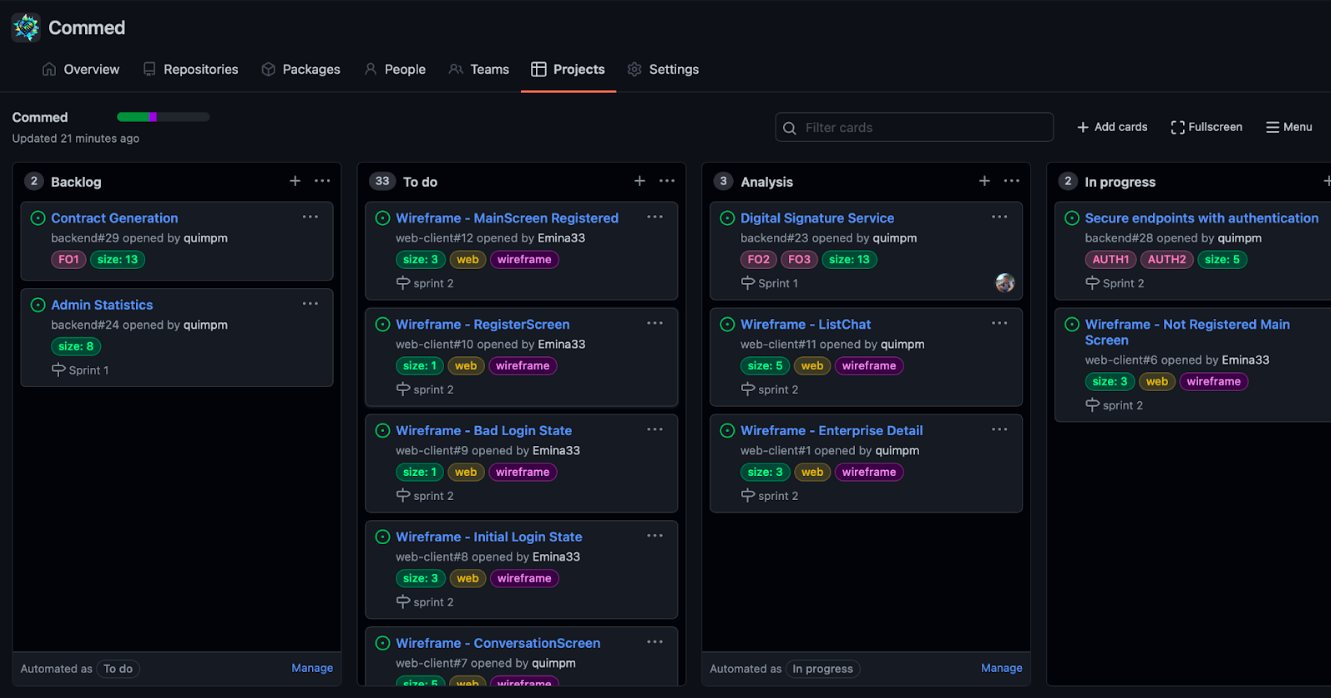
\includegraphics[width=15cm]{img/kanban.png}
	\caption{Screenshot of the first days of the project kanban.}
\end{figure}
\subsubsection{Issues}
\textbf{Backend}
\begin{verbatim}
- List Formal Offers for User
    - size: 3
- List User Products
    - size: 3
- Secure endpoints with authentication
    - size: 5
\end{verbatim}
\textbf{Web client}
\begin{verbatim}
- Wireframe - Publication Detail
    - size: 3
- Wireframe - Profile Detail
    - size: 3
- Wireframe - Enterprise Detail
    - size: 3
- Wireframe - ListChat
    - size: 5
- Wireframe - ConversationScreen
    - size: 5
- Wireframe - ListProducts
    - size: 3
- Wireframe - Not Registered Main Screen
    - size: 3
- Wireframe - MainScreen Registered
    - size: 3
- Wireframe - ListFormalOffer
    - size: 3
- Wireframe - Inital Login State
    - size: 3
- Wireframe - Bad Login State
    - size: 3
- Wireframe - RegisterScreen
    - size: 3
- Wireframe - ListFormalOffer
    - size: 3
- Implementation of Register
    - size: 3
- Implementation of Login
    - size: 3
- Implementation of Product Detail
    - size: 5
- Implementation of 404 NotFoundScreen
    - size: 1
- Implementation of the NavBar
    - size: 3
- Implementation of Home
    - size: 5
- Implementation of Enterprise Detail
    - size: 5
- Implementation of Search Products
    - size: 8
- Implementation of Enterprise Edit
    - size: 5
- Implementation of Edit Product
    - size: 8
- Implementation of Create Product
    - size: 3
- Implementation of Chat
    - size: 8
- Implmentation of Formal Offer List
    - size: 3
- Implementation of Formal Offer Form
    - size: 5
\end{verbatim}
\textbf{Mobile application}
\begin{verbatim}
- Wireframe Planification - State Diagram
    - size: 5
- Wireframe - RegisterScreen
    - size: 2
- Wireframe - Bad Login State
    - size: 1
- Wireframe - Initial Login State
    - size: 2
- Wireframe - Not Registered Main Screen
    - size: 3
- Wireframe - MainScreen Registered
    - size: 5
- Wireframe - PublicationDetail
    - size: 5
- Implementation of Localization Language
    - size: 2
- Implementation and design of Redux architecture
    - size: 13
- Implementation of Copy static method to create a new State in Redux
    - size: 1
- Implementation of RegisterScreen
    - size: 3
- Implementation of LoginScreen
    - size: 5
- Implementation of GenericSummaryWidget
    - size: 2
- Implementation of CarrousleSliderWidget
    - size:  3
- Implementation of Product/Service Publication Screen
    - size: 5
- Implementation of ListChatScreen
    - size: 5
- Implementation of FormalOfferDetailScreen
    - size: 3
- Implementation of ListFormalOfferScreen
    - size: 5
- Implementation of ConversationScreen
    - size: 8
- Implementation of Profile Enterprise Detail Screen
    - size: 3
- Design and Title of the Application - Manifest
    - size: 1
- Implementation of SearcherView
    - size: 5
- Implmentation of Authentication Logic
    - size: 3
- Implementation of MainScreen without registration user
    	- size: 5
\end{verbatim}

\subsection{Scrum analytics}
As Github does not support milestones for a group of repositories but for single one, it has been created three different milestones for each project: \texttt{backend}, \texttt{web-client} and \texttt{mobile-app}.
\\
\\
\textbf{backend}
\begin{figure}[H]
	\centering
	
\includegraphics[width=15cm]{img/sprint2-backend.png}
	\caption{Backend Sprint 2 milestone}
\end{figure}
As it can be seen, the backend has only little modifications, that is why the percentage can be smaller even though it has been done all the tasks for this sprint. The task that is still missing is the authorization management of the endpoints called, which will be held on the next sprint.
\\
\\
\textbf{web-client}
\begin{figure}[H]
	\centering
	
\includegraphics[width=15cm]{img/sprint2-web.png}
	\caption{Web client Sprint 2 milestone}
\end{figure}
In regards of the web client, mostly of the tasks are done. The tasks that are not done are depending on issues detected in backend, such as image management and chat. This issues will be postponed to the third sprint, where will be created new issues related to the back.
\\\\
\textbf{mobile-app}
\begin{figure}[H]
	\centering
	
\includegraphics[width=15cm]{img/sprint2-mobile.png}
	\caption{Web client Sprint 2 milestone}
\end{figure}
According to the mobile application, the things that are still in progress or in to do stage are about the integration of the API backend, which were formerly associated with this sprint. However, while iterating for this sprint, we did realize about that and it was considered that the issues of design and architecture were more important to be finished on this sprint.
%Sprint stuff. Commits estatistics, completition of the tasks, number of tasks done, amount of size completed, sprint progression grapic, Backlog...

\section{Requirements}
In this section the list of requirements that the application has to offer to the user are on the list below. As matter of fact, the requirements have been more detailed in this sprint, the changes and new requirements are written in \textit{italics}.
\\\\
\textbf{Functional Requirements:}
\begin{itemize}
	
	\item
	The application has to let all kinds of users search for products or
	services.
	\item
	The application has to let users register into the application \textit{and it will create automatically an enterprise profile}.
	\item
	The application has to let users log in to the application if they
	have an active account on the system.
	\item
	The application has to let logged users publish products or services \textit{in the web application}.
	\item
	The application has to let logged users interested in either a product
	or a service to start a chat with the owner of it.
	\item
	The application has to let logged users who are owners of a given
	product to chat with said interested users through a chat.
	\item
	The application has to let logged users send a commercial transaction
	contract when an agreement has been reached .
	\item 
	\textit{The application has to let logged users download a commercial transaction
	contract sent by the owner of a product that they are interested.}
	\item
	The application has to let logged users sign a commercial transaction
	contract sent by the owner of a product that they are interested.
	\item
	The application has to generate the evidences for both sides of the
	commercial agreement.
	\item \textit{The application has to let logged users to view a list of the formal offers they are in.}
\end{itemize}
\textbf{Non-Functional Requirements:}
\begin{itemize}
	
	\item
	The application has to be the most usable possible.
	\item
	The application has to be compliant and respect the laws that run in
	each country that it's available in.
	\item
	The application mustn't have large waiting times for the client.
	\item
	The application has to be portable and easy to deploy.
	\item
	The application has to be scalable and always leave the code open to
	the possibility of adding new features in the future.
\end{itemize}


\section{Main use cases}

\begin{figure}[h]
\centering
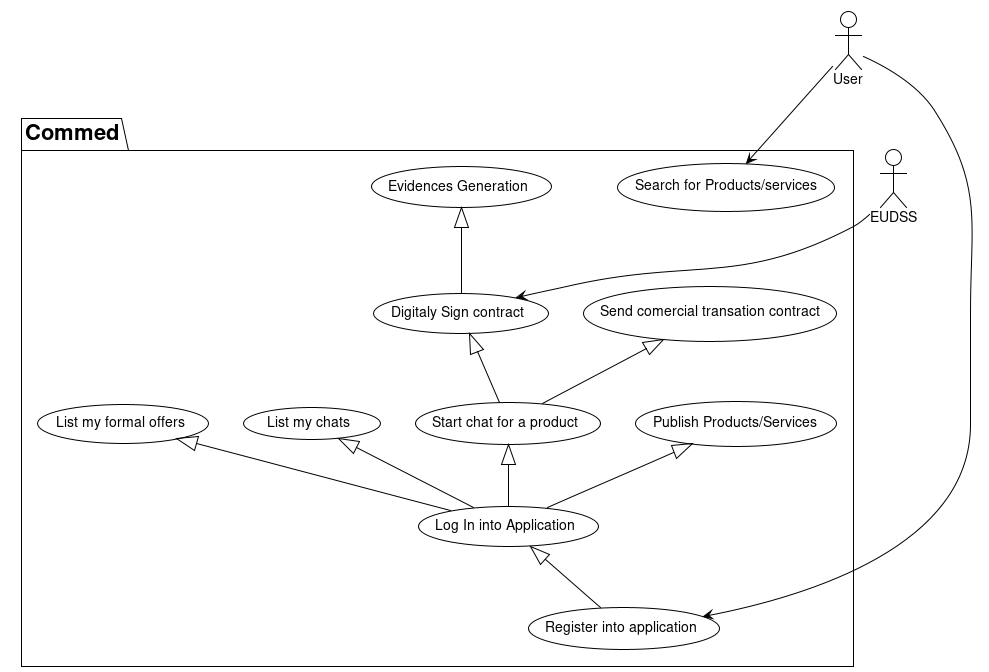
\includegraphics[width=\linewidth]{use_case_diagram/usecase_diagram.png} %TODO Update with new Use Cases file at ./use_case_diagram
\caption{Use case diagram of the application.}
\end{figure}

\subsection{Sprint 1}
\begin{itemize}

\item
  \textbf{Register into application}

  \begin{itemize}
  
  \item
    \textbf{Actors:} User
  \item
    \textbf{Purpose:} Let a user register into the application system
  \item
    \textbf{Description:} Provides a screen with a form in which the
    user is able to fulfill it and send the information to the system in
    order to be registered.
  \end{itemize}
\item
  \textbf{Log In into Application}

  \begin{itemize}
  
  \item
    \textbf{Actors:} User
  \item
    \textbf{Purpose:} Log in to the application to be able to use some
    of the application services.
  \item
    \textbf{Description:} Provides a screen with a form in which the
    user will put its email and password. Then, they will log into the
    application so that they can start using the services that it provides.
  \end{itemize}
\item
  \textbf{Search for Products/services}

  \begin{itemize}
  
  \item
    \textbf{Actors:} User
  \item
    \textbf{Purpose:} Search for any product or service the user is
    interested in.
  \item
    \textbf{Description:} Provides a searcher for every user so that
    they can look up the products or services that they are interested
    in.
  \end{itemize}
\item
  \textbf{Publish Products/Services}

  \begin{itemize}
  
  \item
    \textbf{Actors:} User
  \item
    \textbf{Purpose:} Publish services or products in order to be sold
    to other users.
  \item
    \textbf{Description:} Lets a logged user publish the products and
    services that they offer in order for them to be sold to other
    interested users.
  \end{itemize}
\item
  \textbf{Start chat for a product}

  \begin{itemize}
  
  \item
    \textbf{Actors:} User
  \item
    \textbf{Purpose:} Users can start a chat when they are interested in
    a product
  \item
    \textbf{Description:} Lets a logged user start a chat with the
    owners of either a product or a service that they are interested in,
    so that they can start a negotiation.
  \end{itemize}
\item
  \textbf{Send commercial transaction contract}

  \begin{itemize}
  
  \item
    \textbf{Actors:} User
  \item
    \textbf{Purpose:} Send a formal offer with a commercial transaction
    contract.
  \item
    \textbf{Description:} Lets the owners of given products or services
    send a formal offer containing a compliant commercial transaction
    contract within the chat in which the negotiations are taking place.
  \end{itemize}
\item
  \textbf{Digitally Sign contract}

  \begin{itemize}
  
  \item
    \textbf{Actors:} User EUSSD
  \item
    \textbf{Purpose:} Sign a commercial transaction contract sent within
    a Formal Offer.
  \item
    \textbf{Description:} Lets the users of the application sign
    digitally the contract that was sent as a Formal Offer in the chat
    in which the negotiations took place.
  \end{itemize}
\item
  \textbf{Evidences Generation}

  \begin{itemize}
  
  \item
    \textbf{Actors:} User
  \item
    \textbf{Purpose:} Provide users with evidences and the billing of a
    business transaction
  \item
    \textbf{Description:} The system will generate for both parts the
    commercial transaction with all the evidences and the billing of
    the contract.
  \end{itemize}
\end{itemize}

\subsection{Sprint 2}
%TODO: Add new Sprint 2 Use Cases Here

\hypertarget{general-architecture}{%
\section{General architecture}\label{general-architecture}}

\begin{figure}[H]
\centering
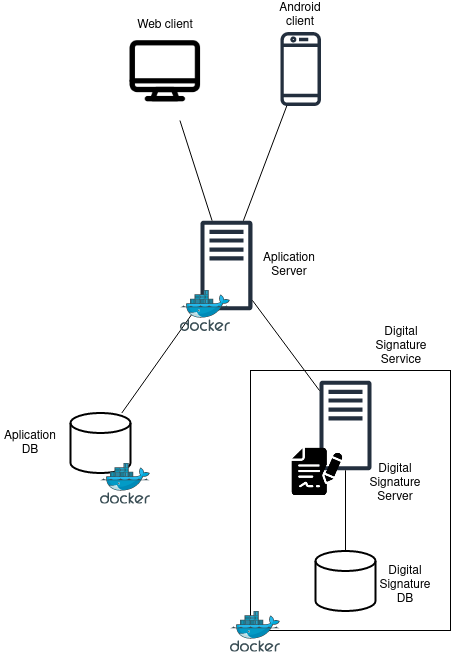
\includegraphics[width=0.6\textwidth]{architecture_diagram/Architecture.drawio.png}
\caption{General architecture of the application.}
\end{figure}

\subfile{mobile.tex} % TODO Add in these files
\subfile{frontend.tex} % TODO Add in these files - Done to review

\section{Database model}
The database model can be seen at figure \ref{fig:model-uml}.

\begin{figure}[H]
\centering
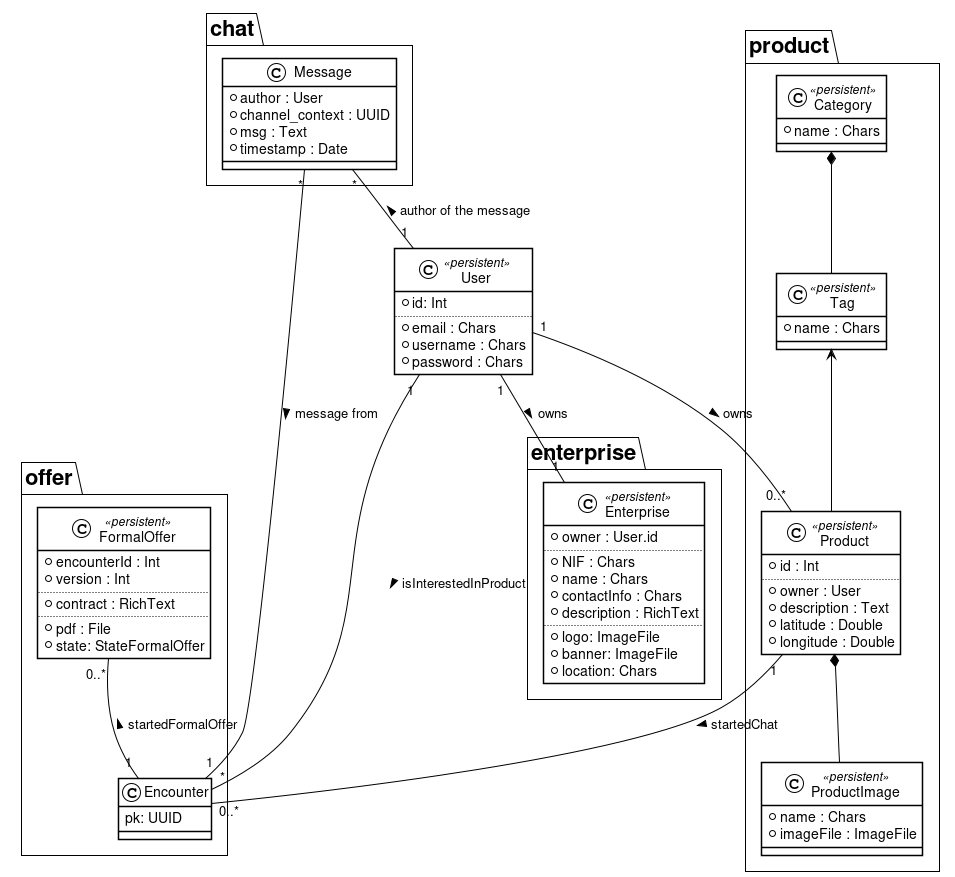
\includegraphics[width=\linewidth]{img/database-model-new.png}
\caption{UML diagram of the models.}
\label{fig:model-uml}
\end{figure}

\subsection{Modifications on the models}
During the implementation of the clients, it was found the lack of the title of the product. As it was discovered in early ages of the sprint, it has been created an issue for it. Also, it was found the lack of an image that would represent the logo of the enterprise and an another one which would correspond to the banner.
\section{Main Screens} \label{sec:views}
In the first stage of the designing of the mobile application, it was held a state diagram to start representing the management and the navigation of the user. This diagram can be shown in \ref{fig:stateapp}.
\begin{figure}
	\centering
	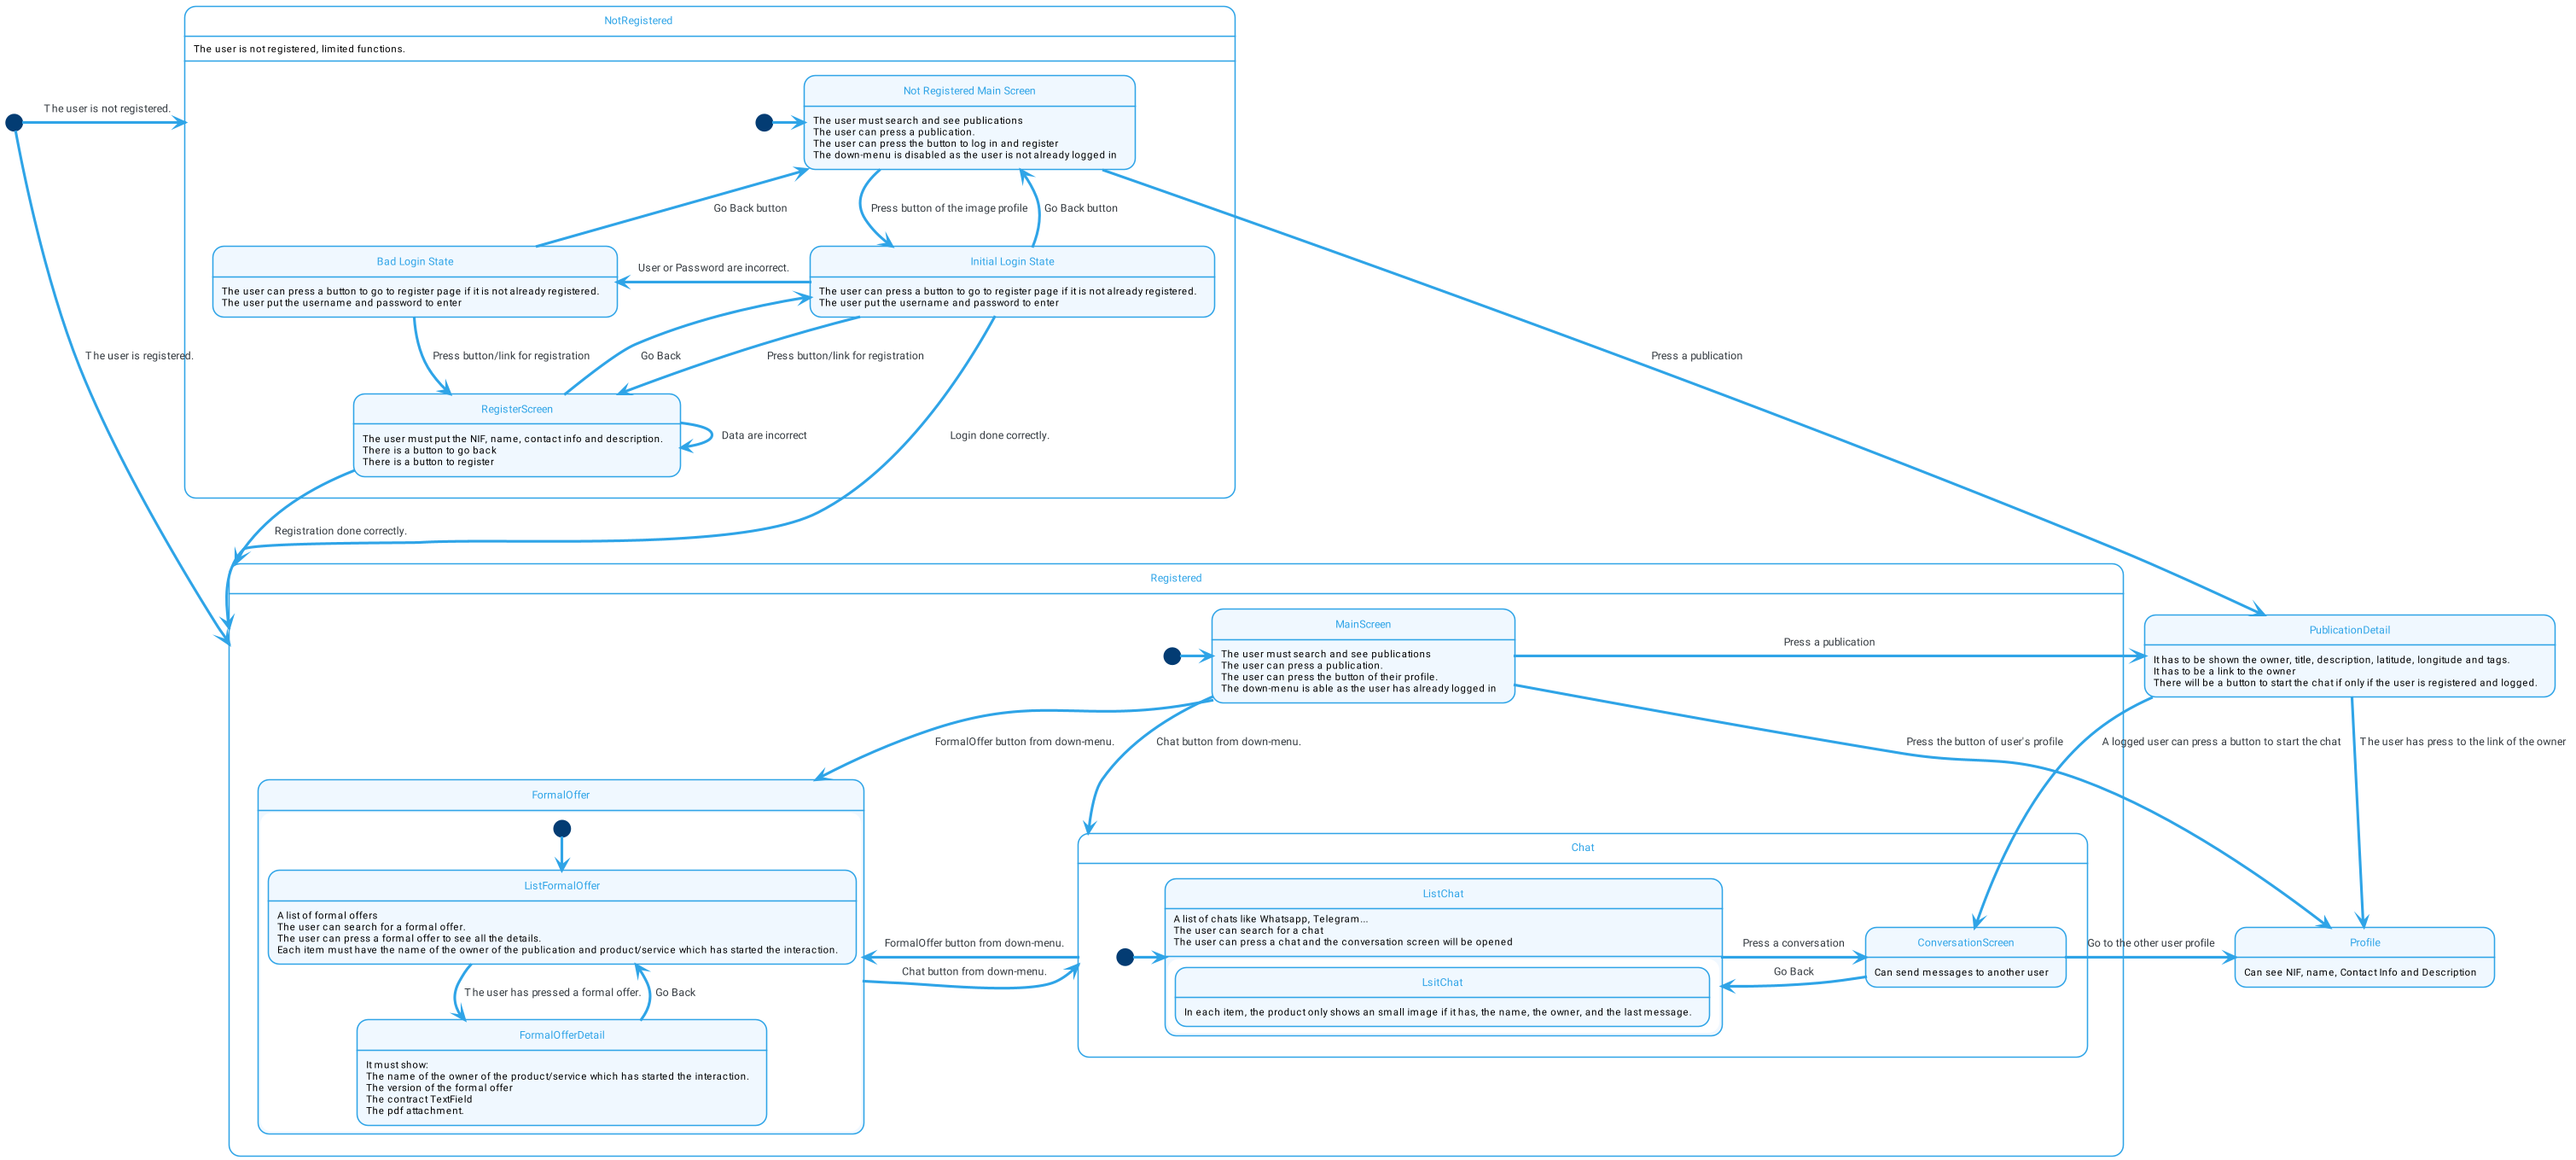
\includegraphics[width=14cm]{stateapp.png}
	\label{fig:stateapp}
	\caption{State diagram of the application.}
\end{figure}
\subsection{Mobile Application}
%TODO: Mobile Application screens.
\subsubsection{Wireframe}
It can be seen in the next images the main screens of the wireframe. At first, it can be seen a list of product
as the main page of the application, in the image \ref{fig:wire-1}. The next image \ref{fig:wire-2} contains the login screen, which can be accessed by clicking on the user icon the image before. The register \ref{fig:wire-3} is accessed by clicking at the sign-up option.\\
\\
The image \ref{fig:wire-4} contains the list of chats that you currently have for every product or service, and the \ref{fig:wire-5} has the detail of a particular chat, that can be seen when clicking in a item from the list of chats. The next image contains the list of formal offers \ref{fig:wire-6}. Both lists can be accessed when clicking on the icon in the bottom menu if the application.\\
\\
The last two images contains the detail of an enterprise \ref{fig:wire-7} and a submenu for things related to the user \ref{fig:wire-8}. The first image can be accessed when clicking the logo of an enterprise, and the last one can be seen when clicking on the user logo. 
\begin{figure}[H]
	\centering
	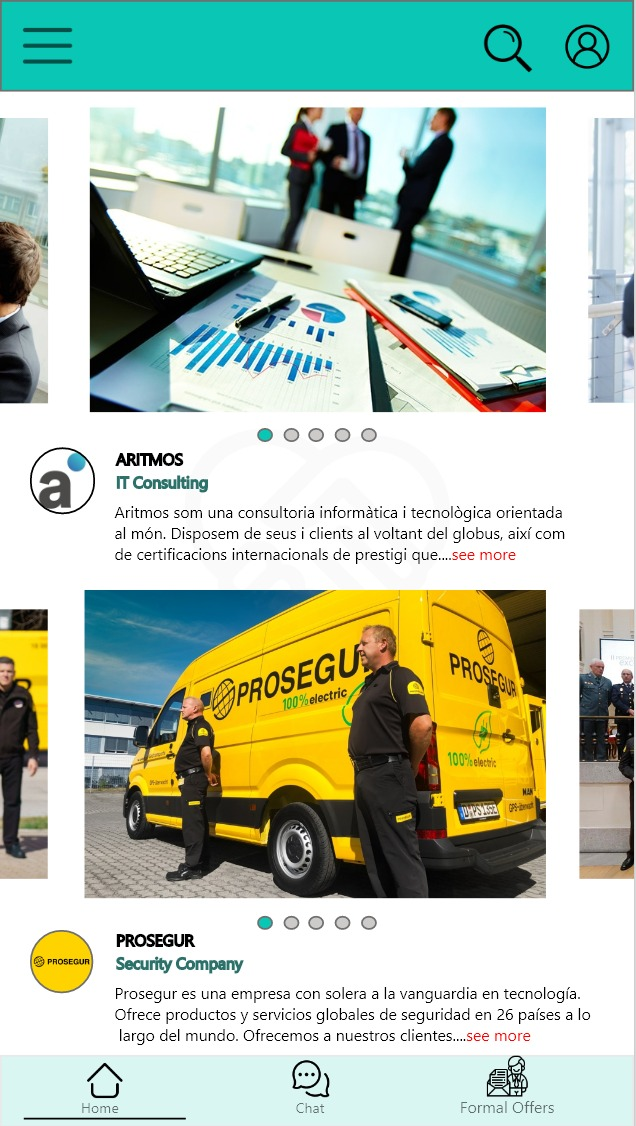
\includegraphics[width=0.5\linewidth]{img/home-page.jpeg}
	\caption{Home mobile screen, it lists the products}
	\label{fig:wire-1}
\end{figure}

\begin{figure}[H]
	\centering
	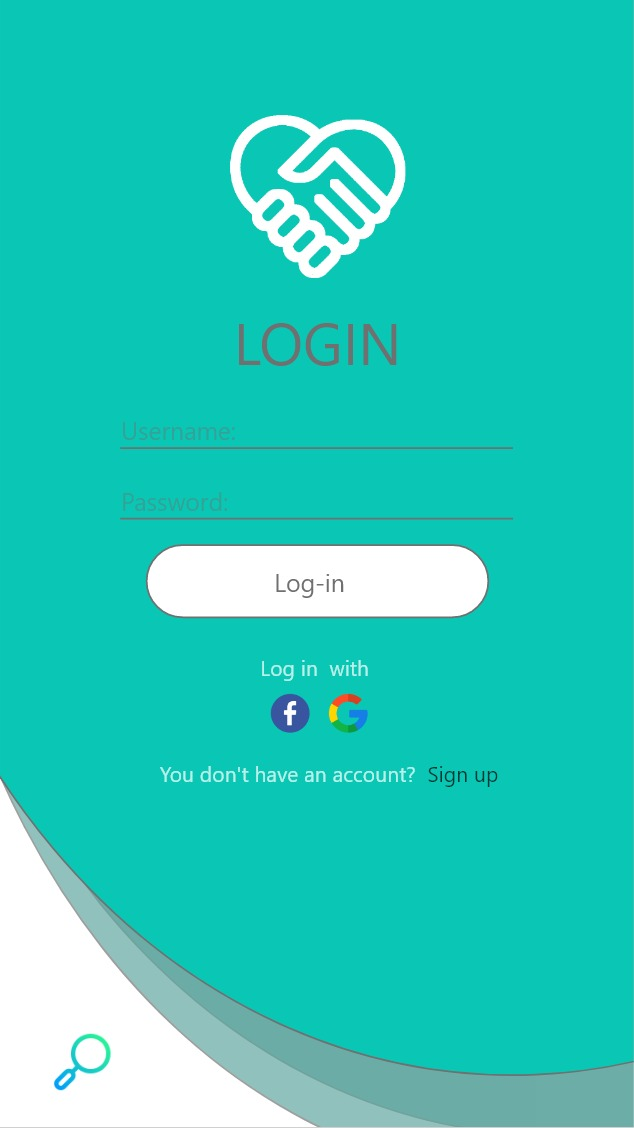
\includegraphics[width=0.5\linewidth]{img/login-page.jpeg}
	\caption{Login view}
\label{fig:wire-2}
\end{figure}

\begin{figure}[H]
	\centering
	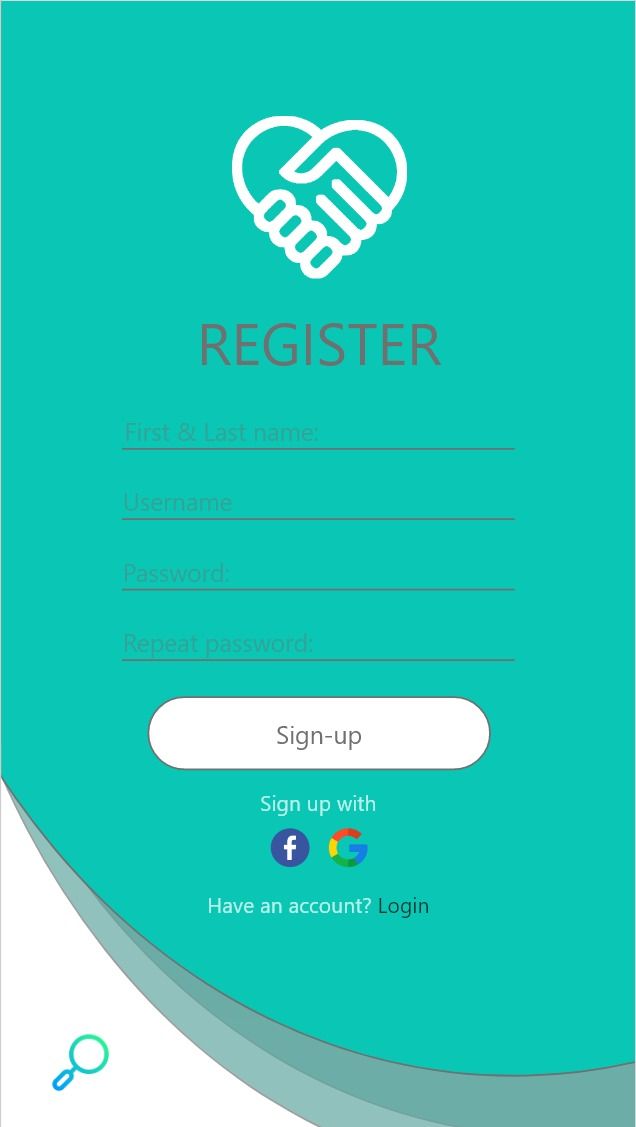
\includegraphics[width=0.5\linewidth]{img/register-page.jpeg}
	\caption{Register view}
	\label{fig:wire-3}
\end{figure}

\begin{figure}[H]
	\centering
	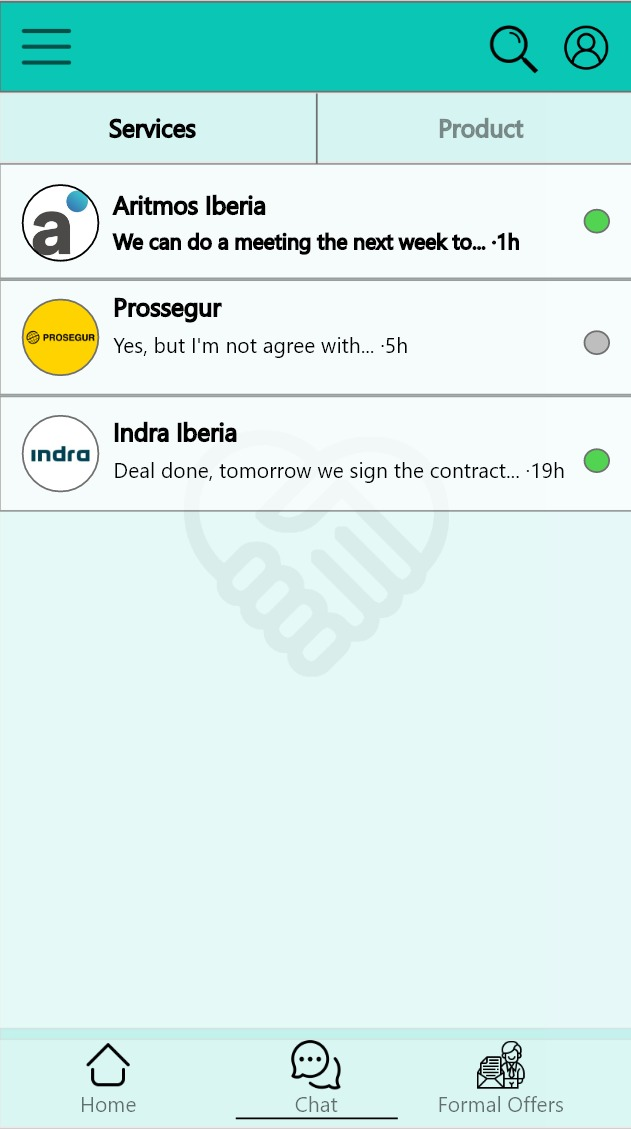
\includegraphics[width=0.5\linewidth]{img/chat-list.jpeg}
	\caption{List of the current chats.}
	\label{fig:wire-4}
\end{figure}

\begin{figure}[H]
	\centering
	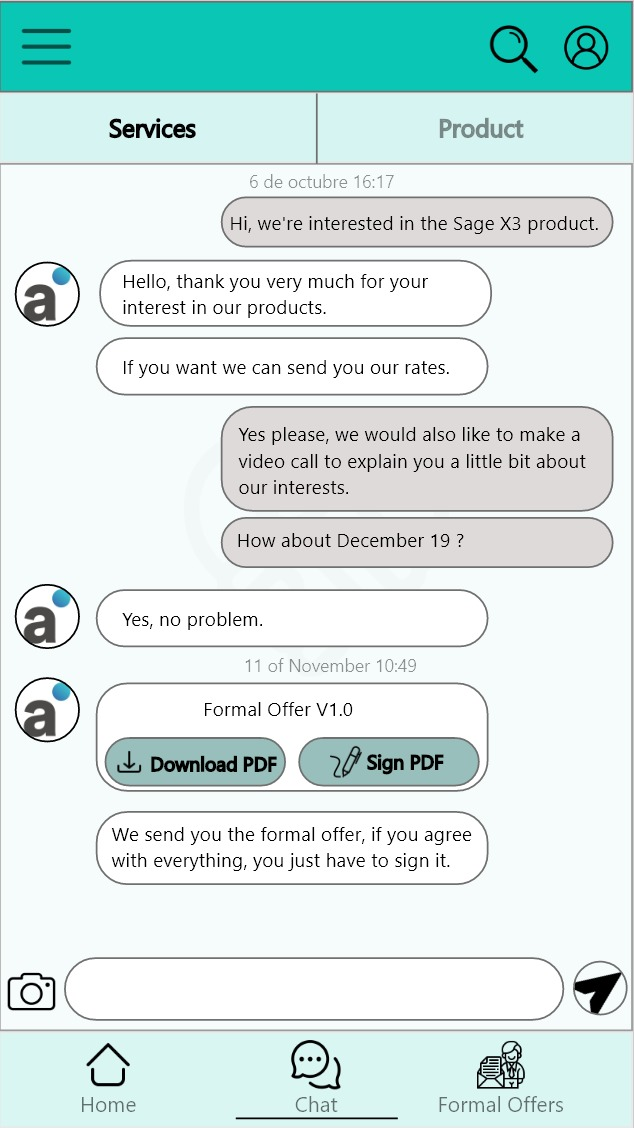
\includegraphics[width=0.5\linewidth]{img/chat-conversation.jpeg}
	\caption{A chat conversation.}
	\label{fig:wire-5}
\end{figure}

\begin{figure}[H]
	\centering
	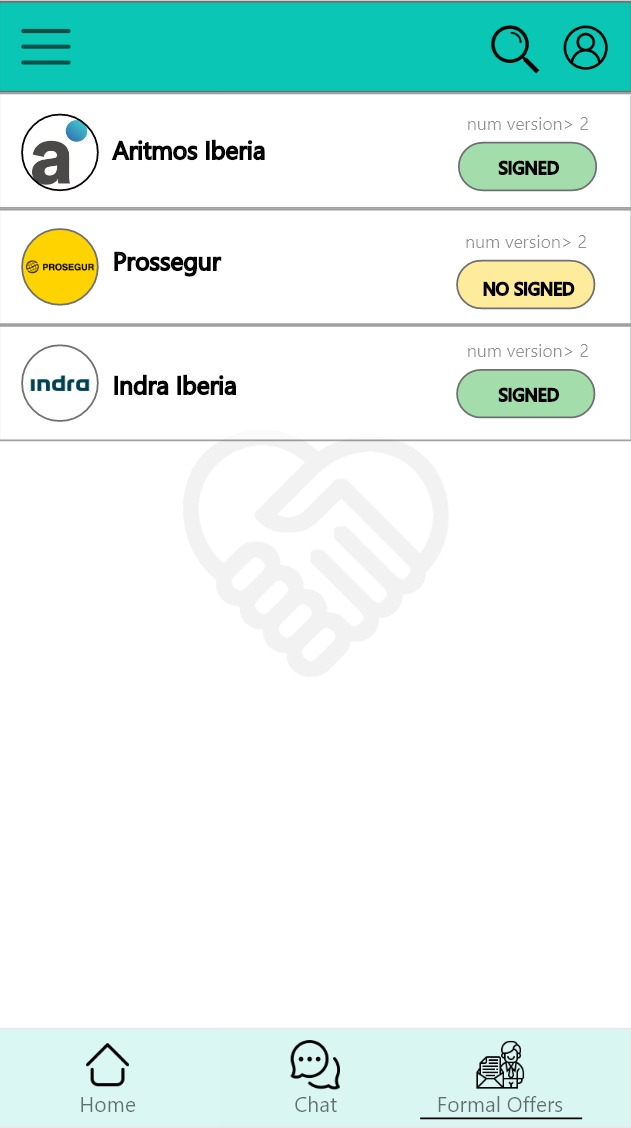
\includegraphics[width=0.5\linewidth]{img/formal-offers.jpeg}
	\caption{List of formal offers.}
	\label{fig:wire-6}
\end{figure}

\begin{figure}[H]
	\centering
	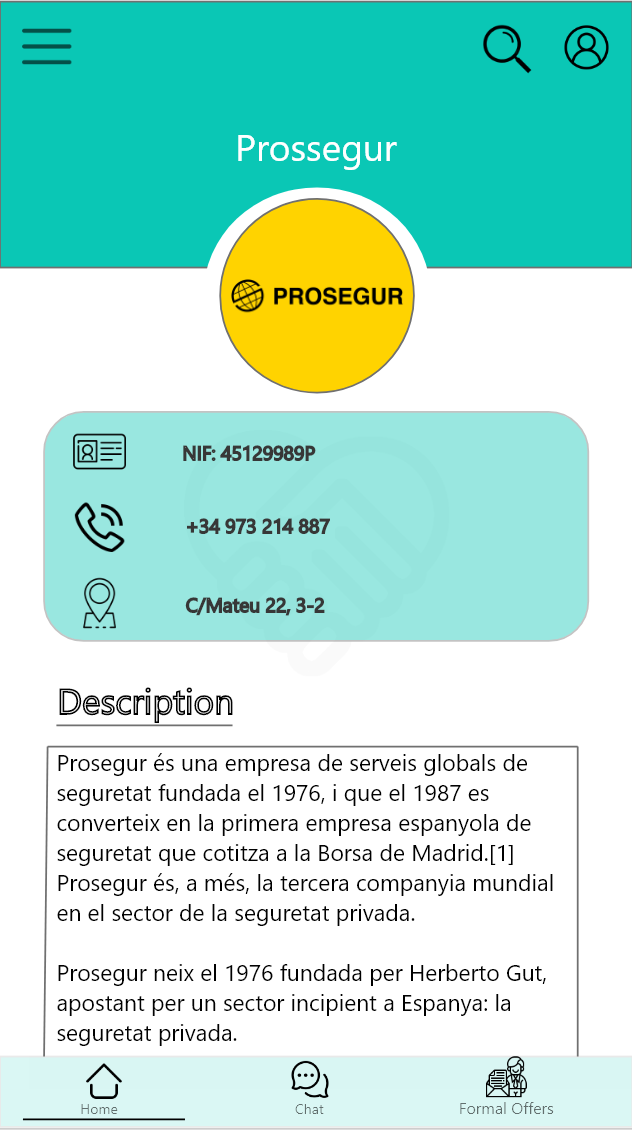
\includegraphics[width=0.5\linewidth]{img/enterprise-profile.png}
	\caption{An enterprise profile.}
	\label{fig:wire-7}
\end{figure}

\begin{figure}[H]
	\centering
	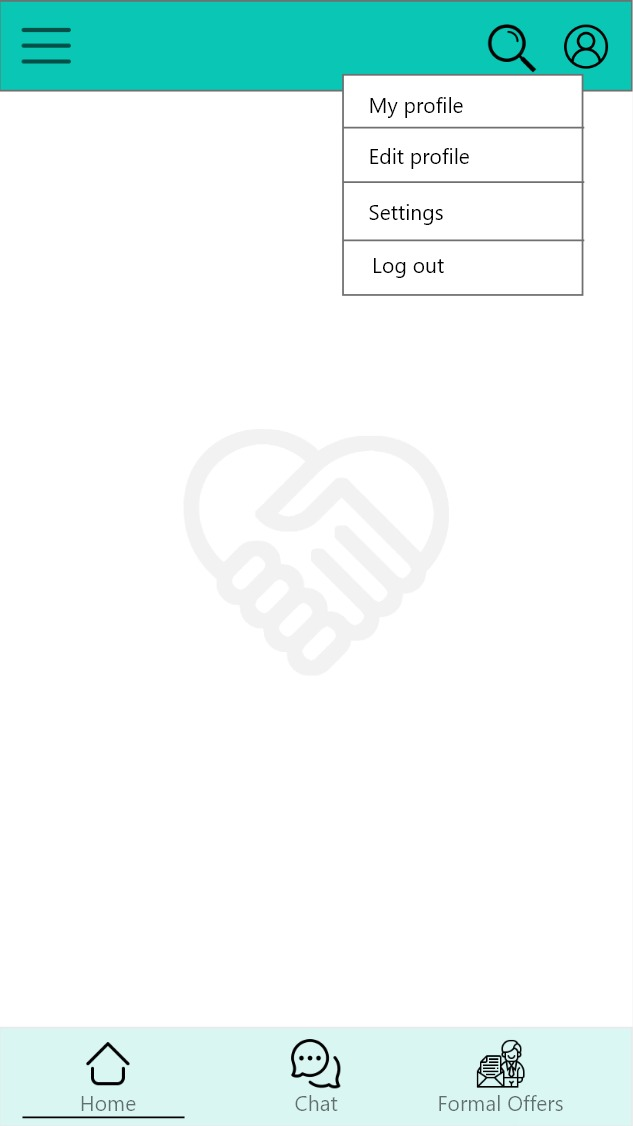
\includegraphics[width=0.5\linewidth]{img/menu-profile.jpeg}
	\caption{Menu Profile.}
	\label{fig:wire-8}
\end{figure}


\subsubsection{Application}
In this section, you will encounter all the screens that the application has currently. The first three images correspond to the home, which lists some products, the list of chats, and the list of formal offers. This can be accessed when clicking at the bottom view. It can not be slides, as it was found confusing when using the images' carousel.\\
\\
The next page \ref{fig:mobile-screen-5} is the profile of an enterprise, which is triggered when clicking a logo of the enterprise, in the pages before. In the figure \ref{fig:mobile-screen-4}, the chat between two users can be seen. It also can be seen a formal offer version, and although a formal offer version can only be send by the owner of the product, it was though that showcasing both items in the mock would be better. The next image \ref{fig:mobile-screen-3} is the searcher of the app, that can be triggered when clicking the magnifying  glass icon. It has the history of the items searched, which can be deleted when clicking the trash button, or replicated when clicking the text.\\
\\
Finally, in the images \ref{fig:mobile-screen-2}, \ref{fig:mobile-screen-1}, it is shown the registration and the login screens.
\begin{figure}[H]
	\centering
	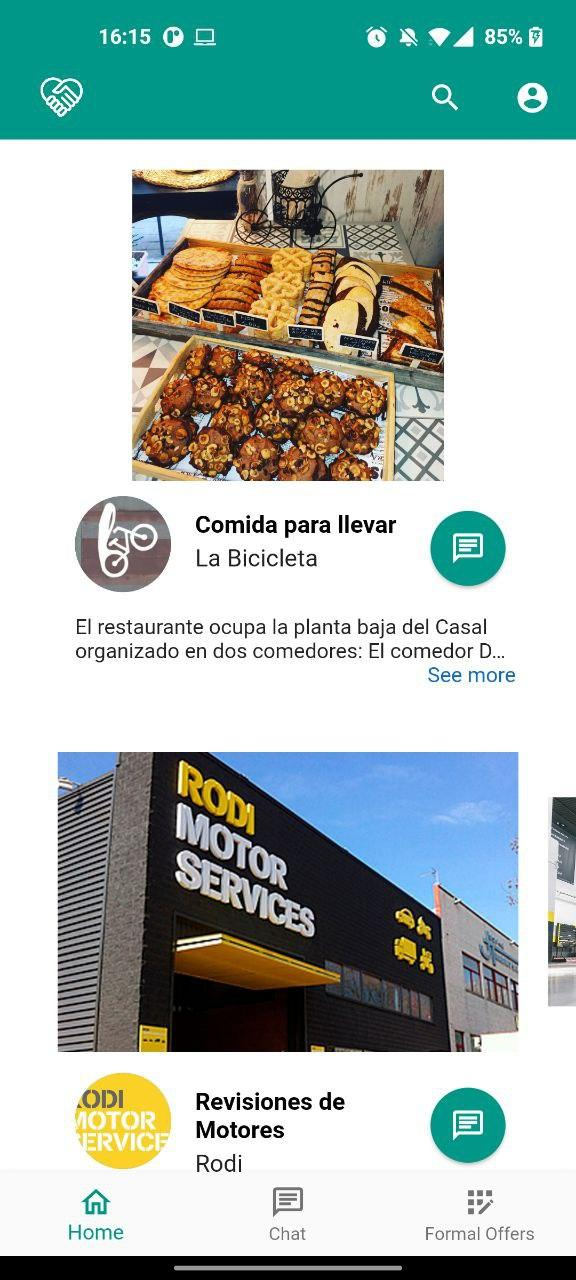
\includegraphics[width=0.5\linewidth]{img/mobile-screen-8.jpg}
	\caption{Home mobile screen, it lists the products}
	\label{fig:mobile-screen-8}
\end{figure}
\begin{figure}[H]
\centering
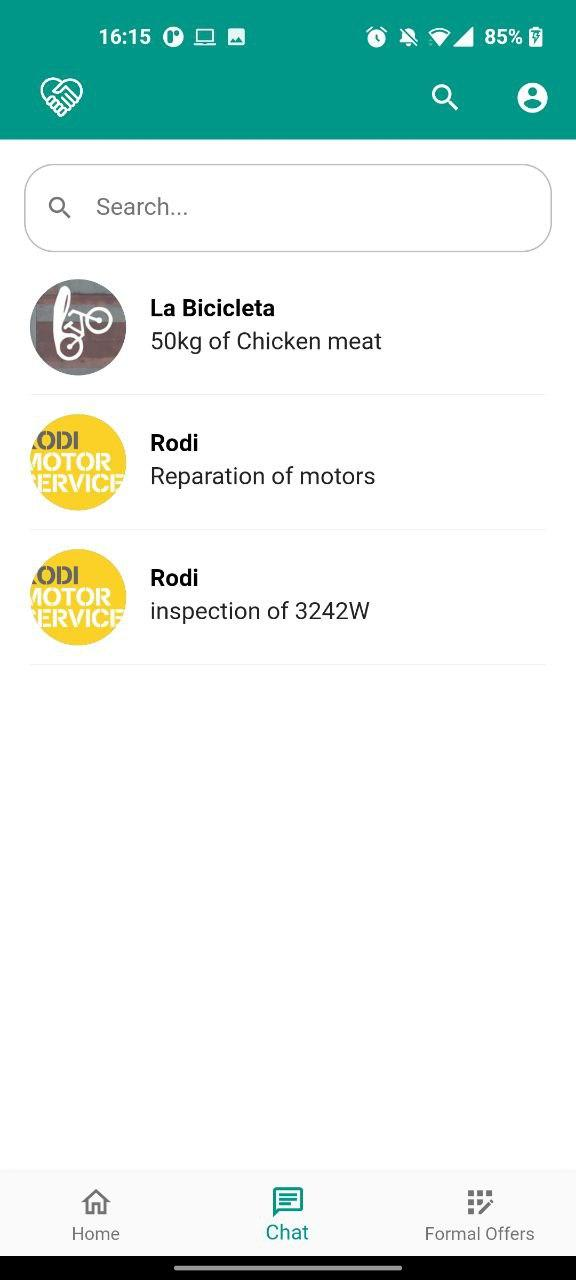
\includegraphics[width=0.5\linewidth]{img/mobile-screen-7.jpg}
\caption{List of the current chats.}
\label{fig:mobile-screen-7}
\end{figure}
\begin{figure}[H]
\centering
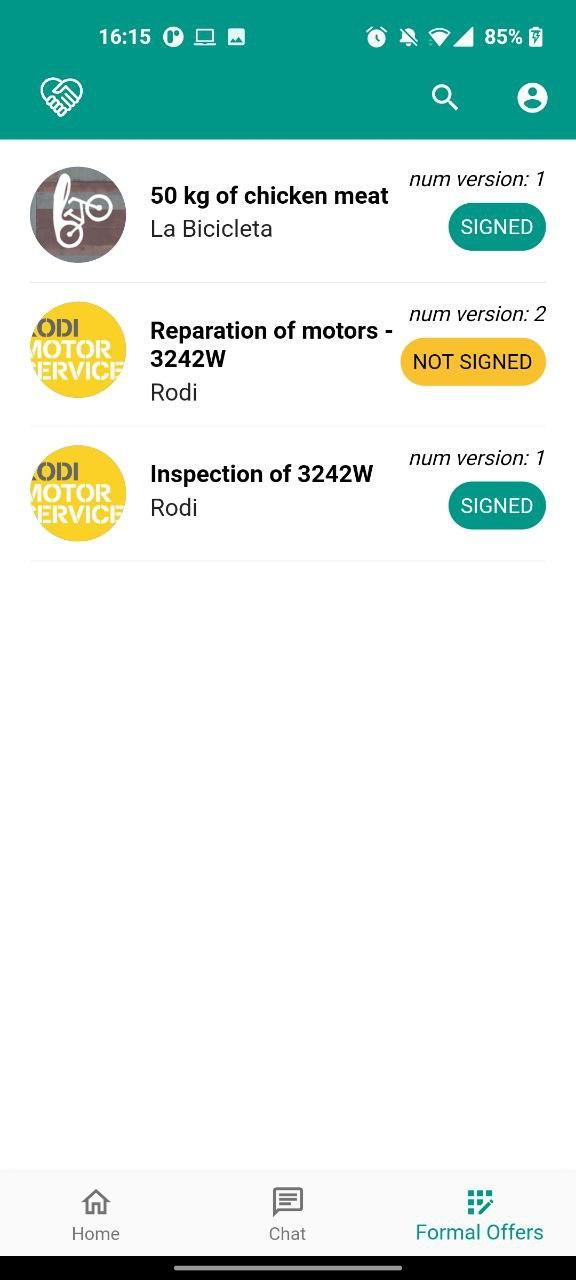
\includegraphics[width=0.5\linewidth]{img/mobile-screen-6.jpg}
\caption{List of the current formal offers.}
\label{fig:mobile-screen-6}
\end{figure}
\begin{figure}[H]
\centering
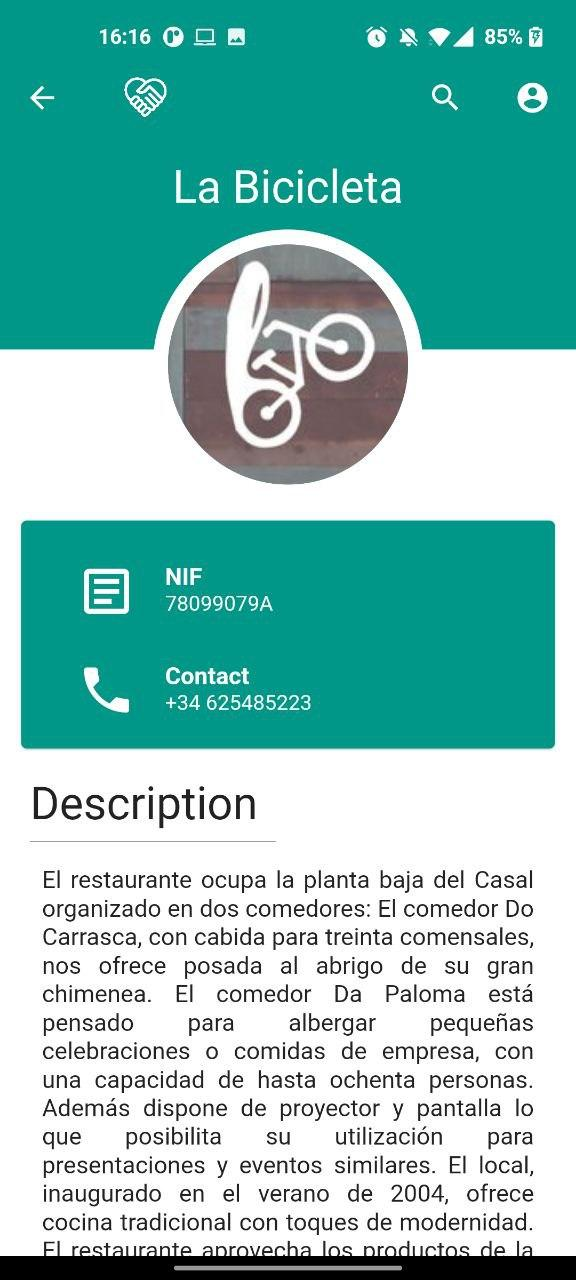
\includegraphics[width=0.5\linewidth]{img/mobile-screen-5.jpg}
\caption{Detail of an enterprise, it can be found when clicking the logo of it.}
\label{fig:mobile-screen-5}
\end{figure}
\begin{figure}[H]
\centering
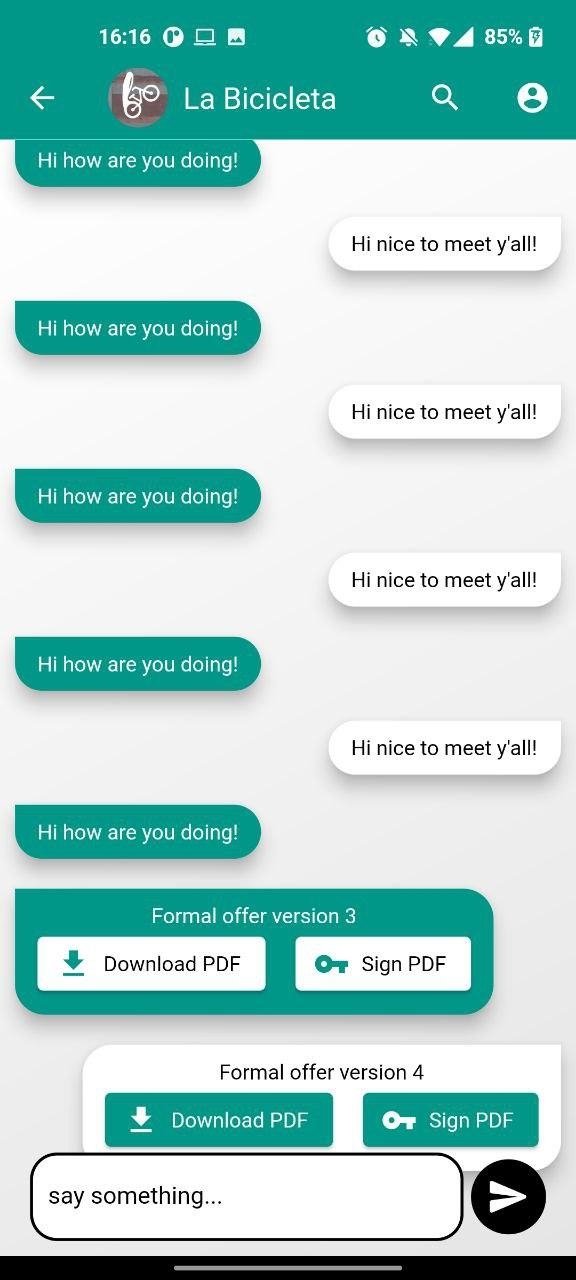
\includegraphics[width=0.5\linewidth]{img/mobile-screen-4.jpg}
\caption{Chat screen.}
\label{fig:mobile-screen-4}
\end{figure}
\begin{figure}[H]
\centering
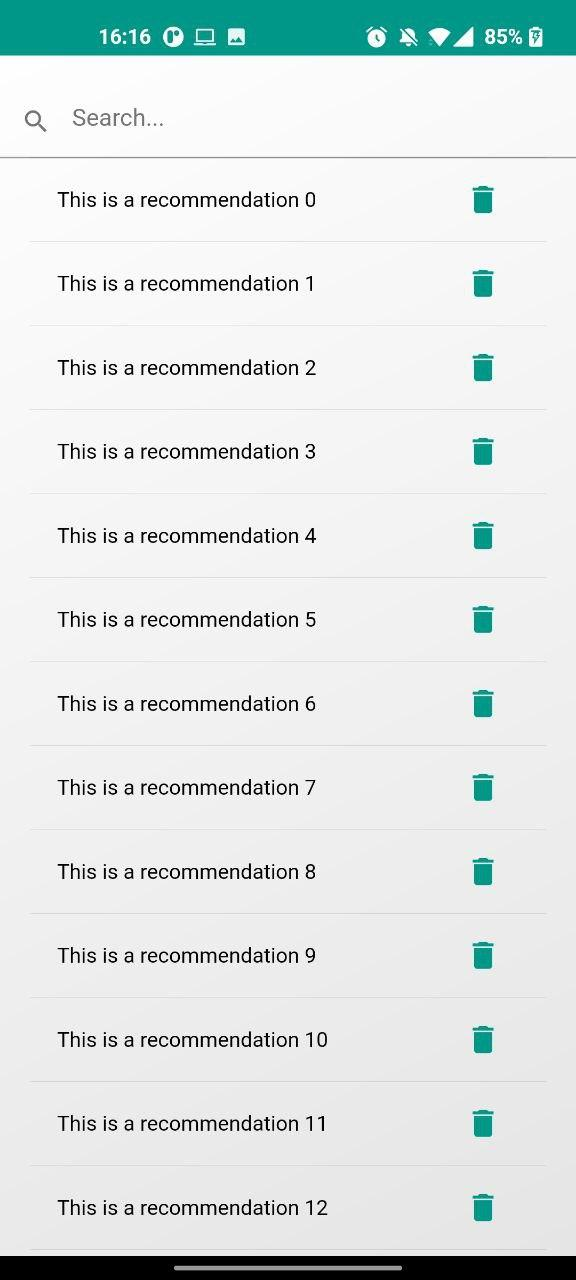
\includegraphics[width=0.5\linewidth]{img/mobile-screen-3.jpg}
\caption{Recommendations screen.}
\label{fig:mobile-screen-3}
\end{figure}
\begin{figure}[H]
\centering
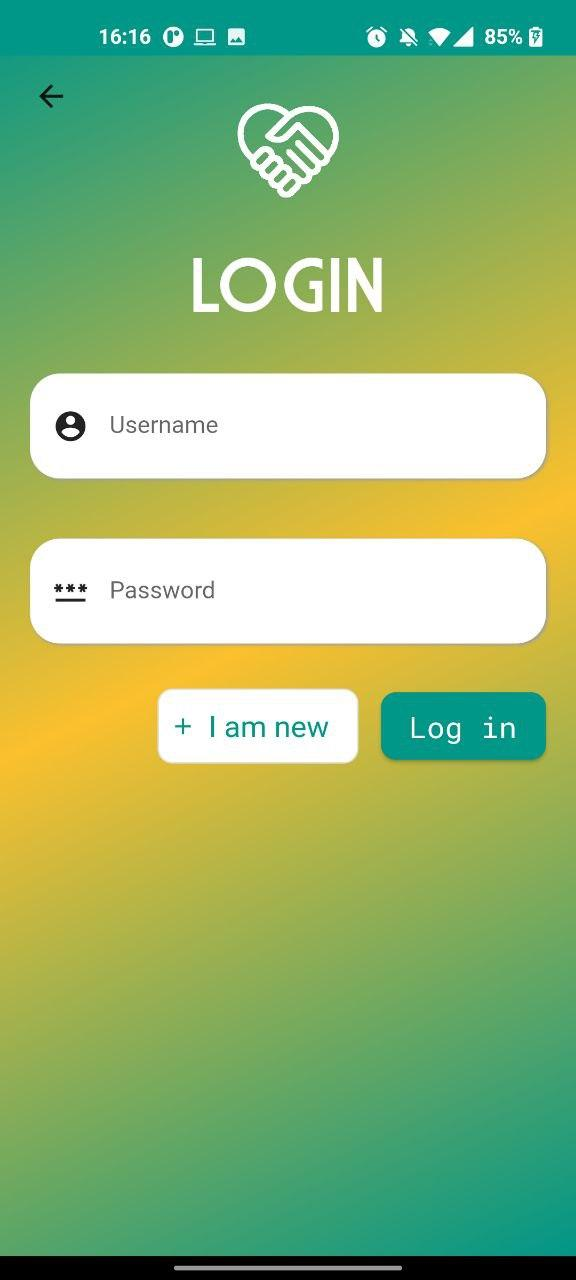
\includegraphics[width=0.5\linewidth]{img/mobile-screen-2.jpg}
\caption{Login view.}
\label{fig:mobile-screen-2}
\end{figure}
\begin{figure}[H]
\centering
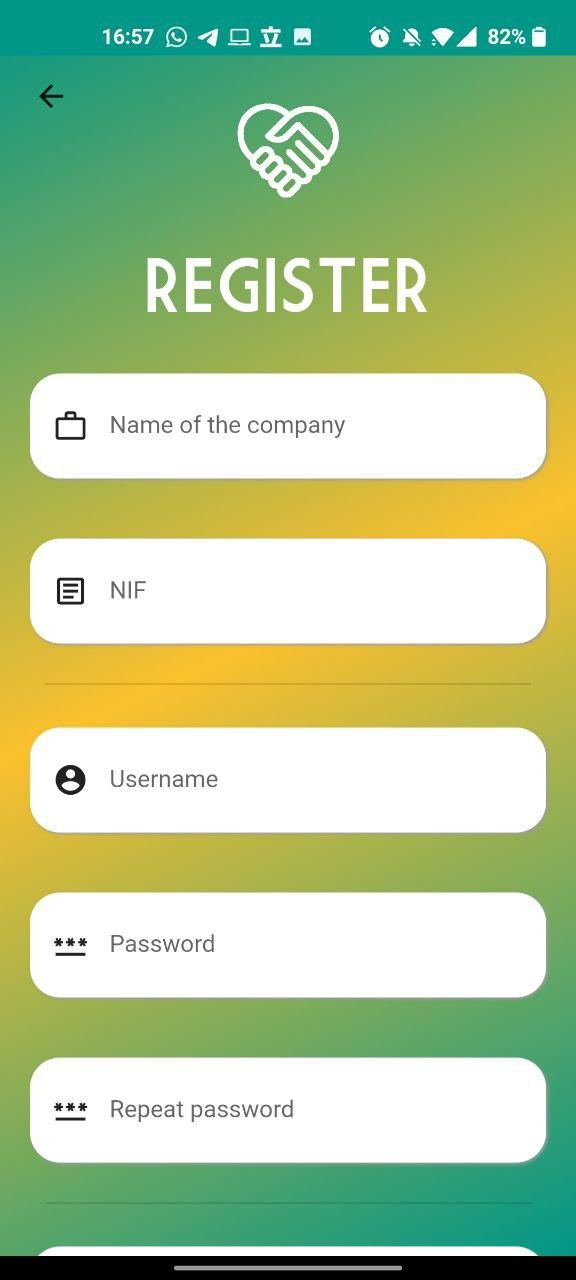
\includegraphics[width=0.5\linewidth]{img/mobile-screen-1.jpg}
\caption{Registration screen.}
\label{fig:mobile-screen-1}
\end{figure}


\subsection{Web Client}

\subsubsection{Wireframe}
In this section, it is going to be shown the paper wireframe that was drawn. This contains the first ideas that had been thought for the dessign of the web application.
\begin{figure}[H]
  \centering
  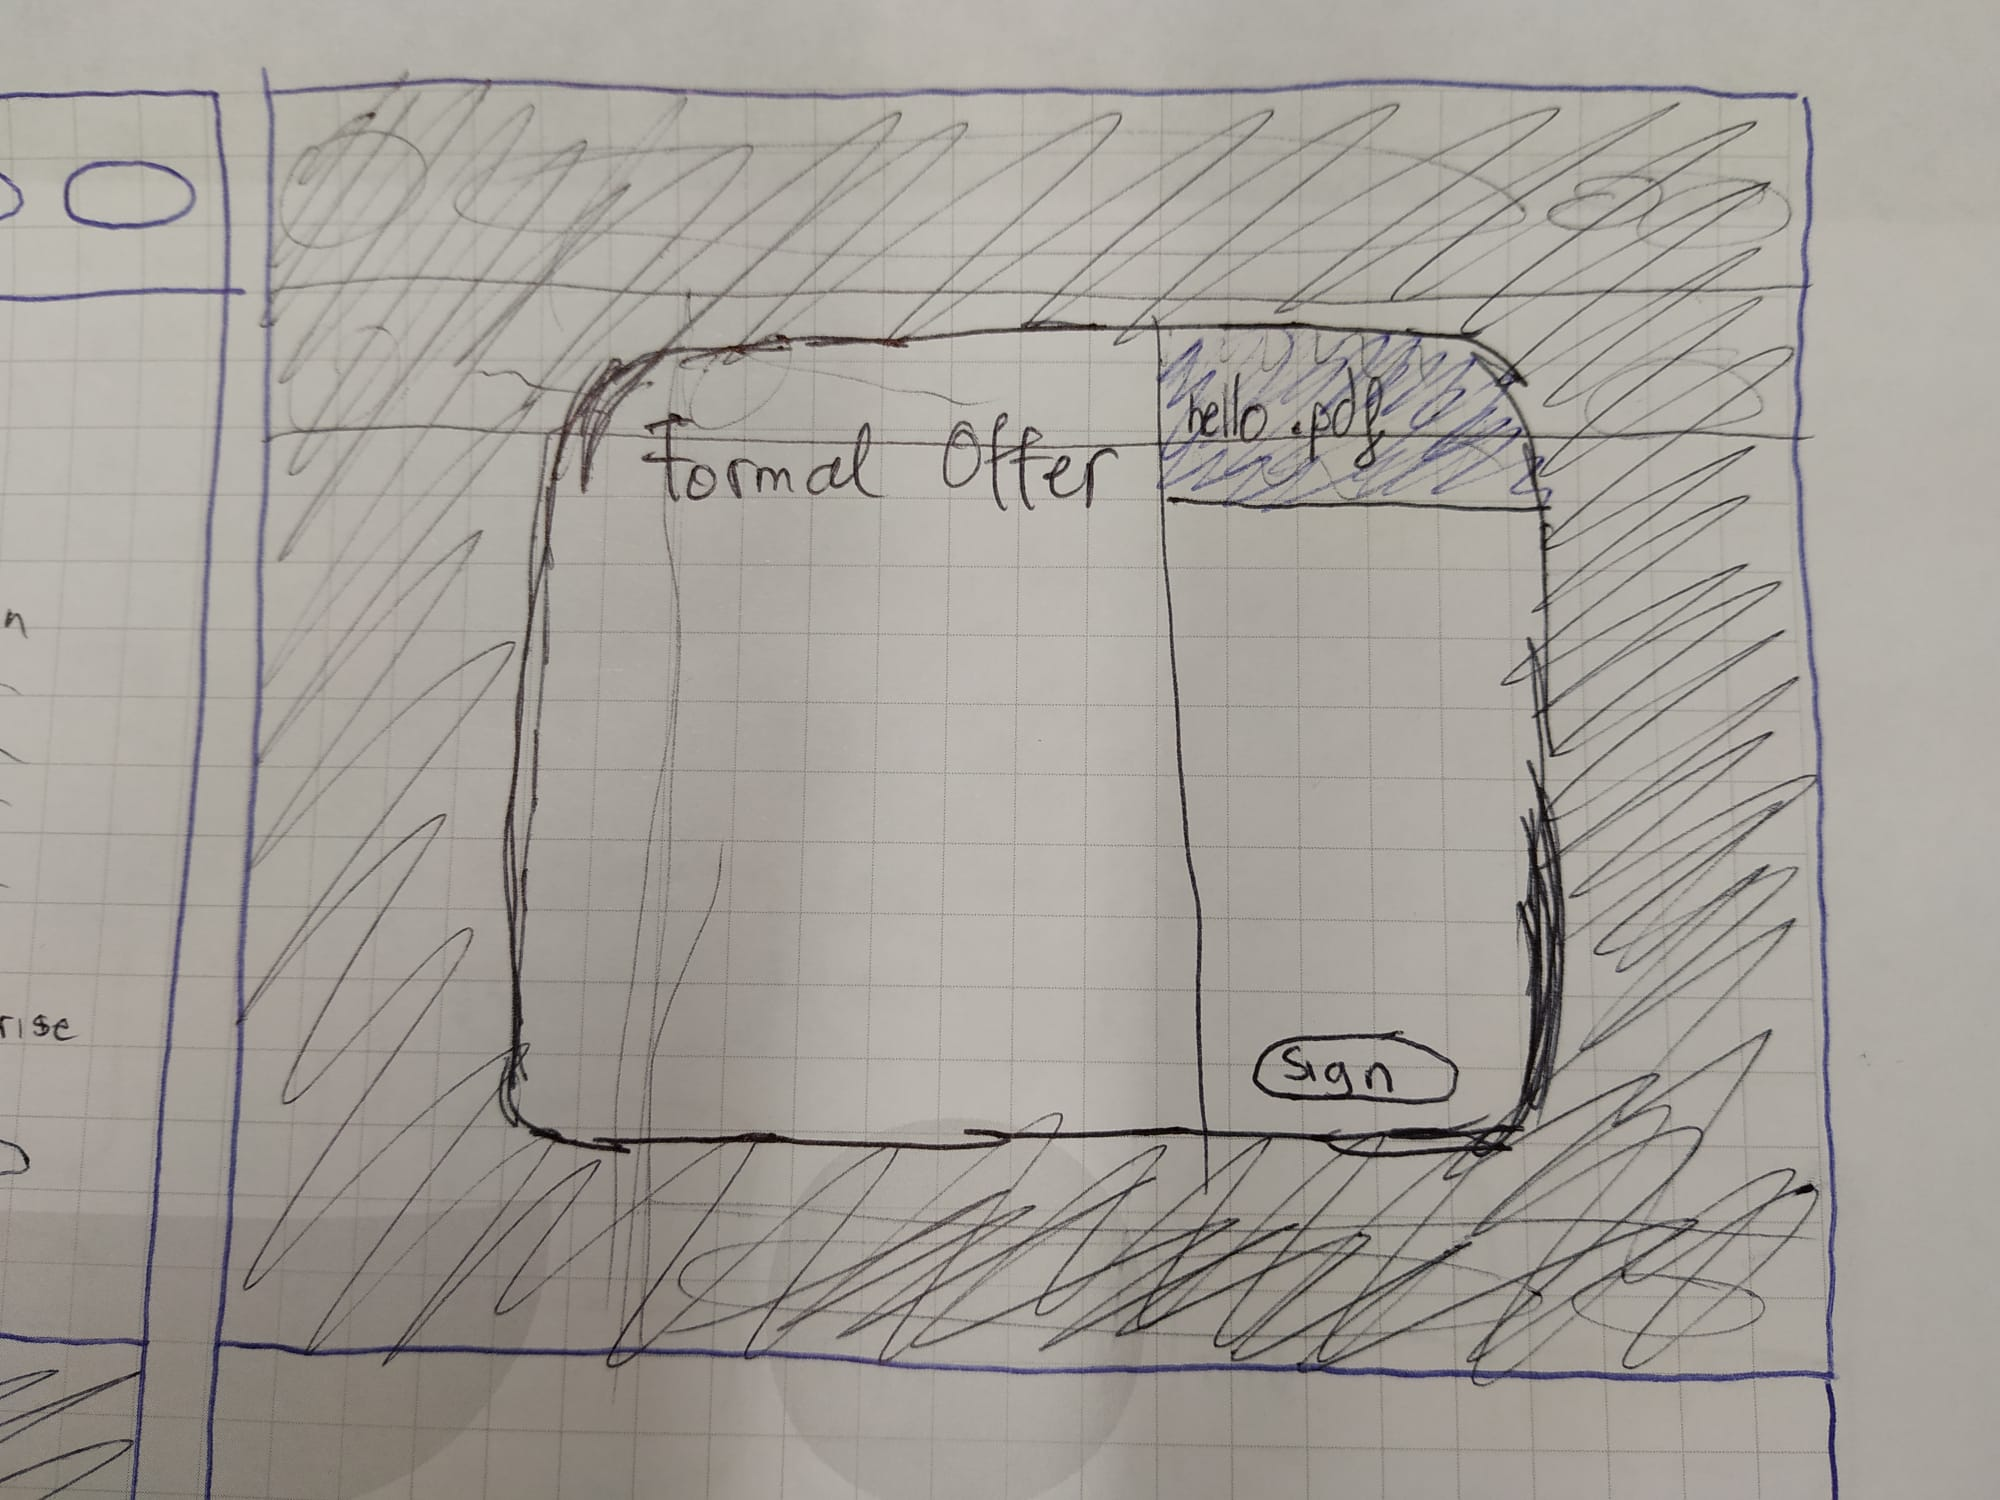
\includegraphics[width=0.5\linewidth]{img/webwire_1.jpeg}
  \caption{FormalOffer Detail Sign screen.}
  \label{fig:webwire-screen-1}
\end{figure}
\begin{figure}[H]
  \centering
  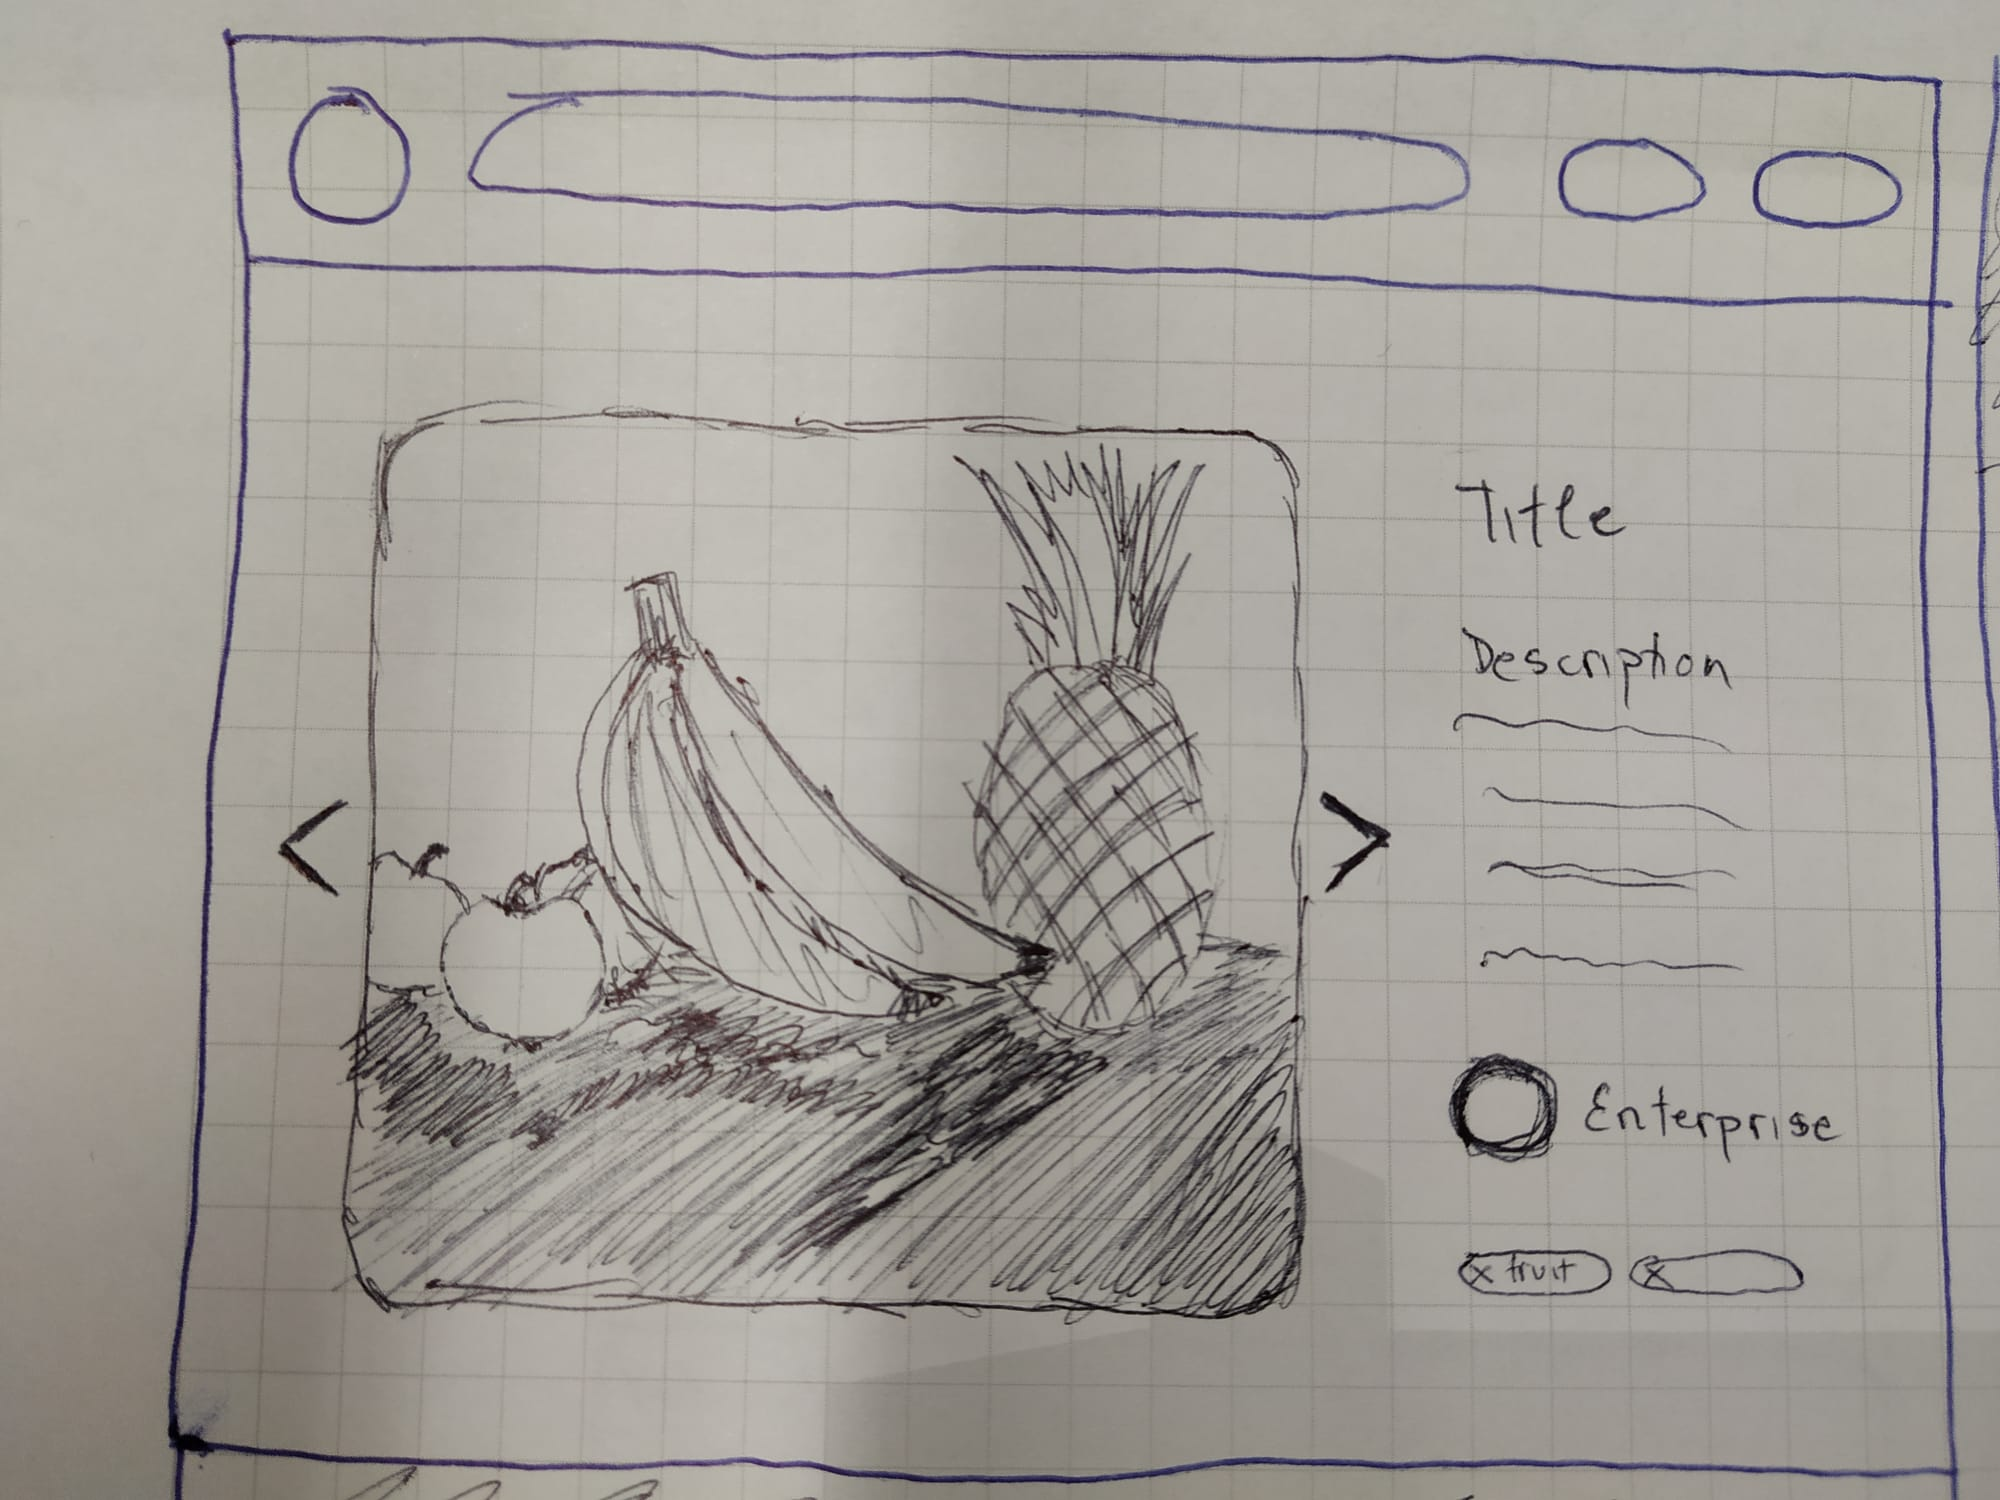
\includegraphics[width=0.5\linewidth]{img/webwire_2.jpeg}
  \caption{Product Detail screen.}
  \label{fig:webwire-screen-1}
\end{figure}
\begin{figure}[H]
  \centering
  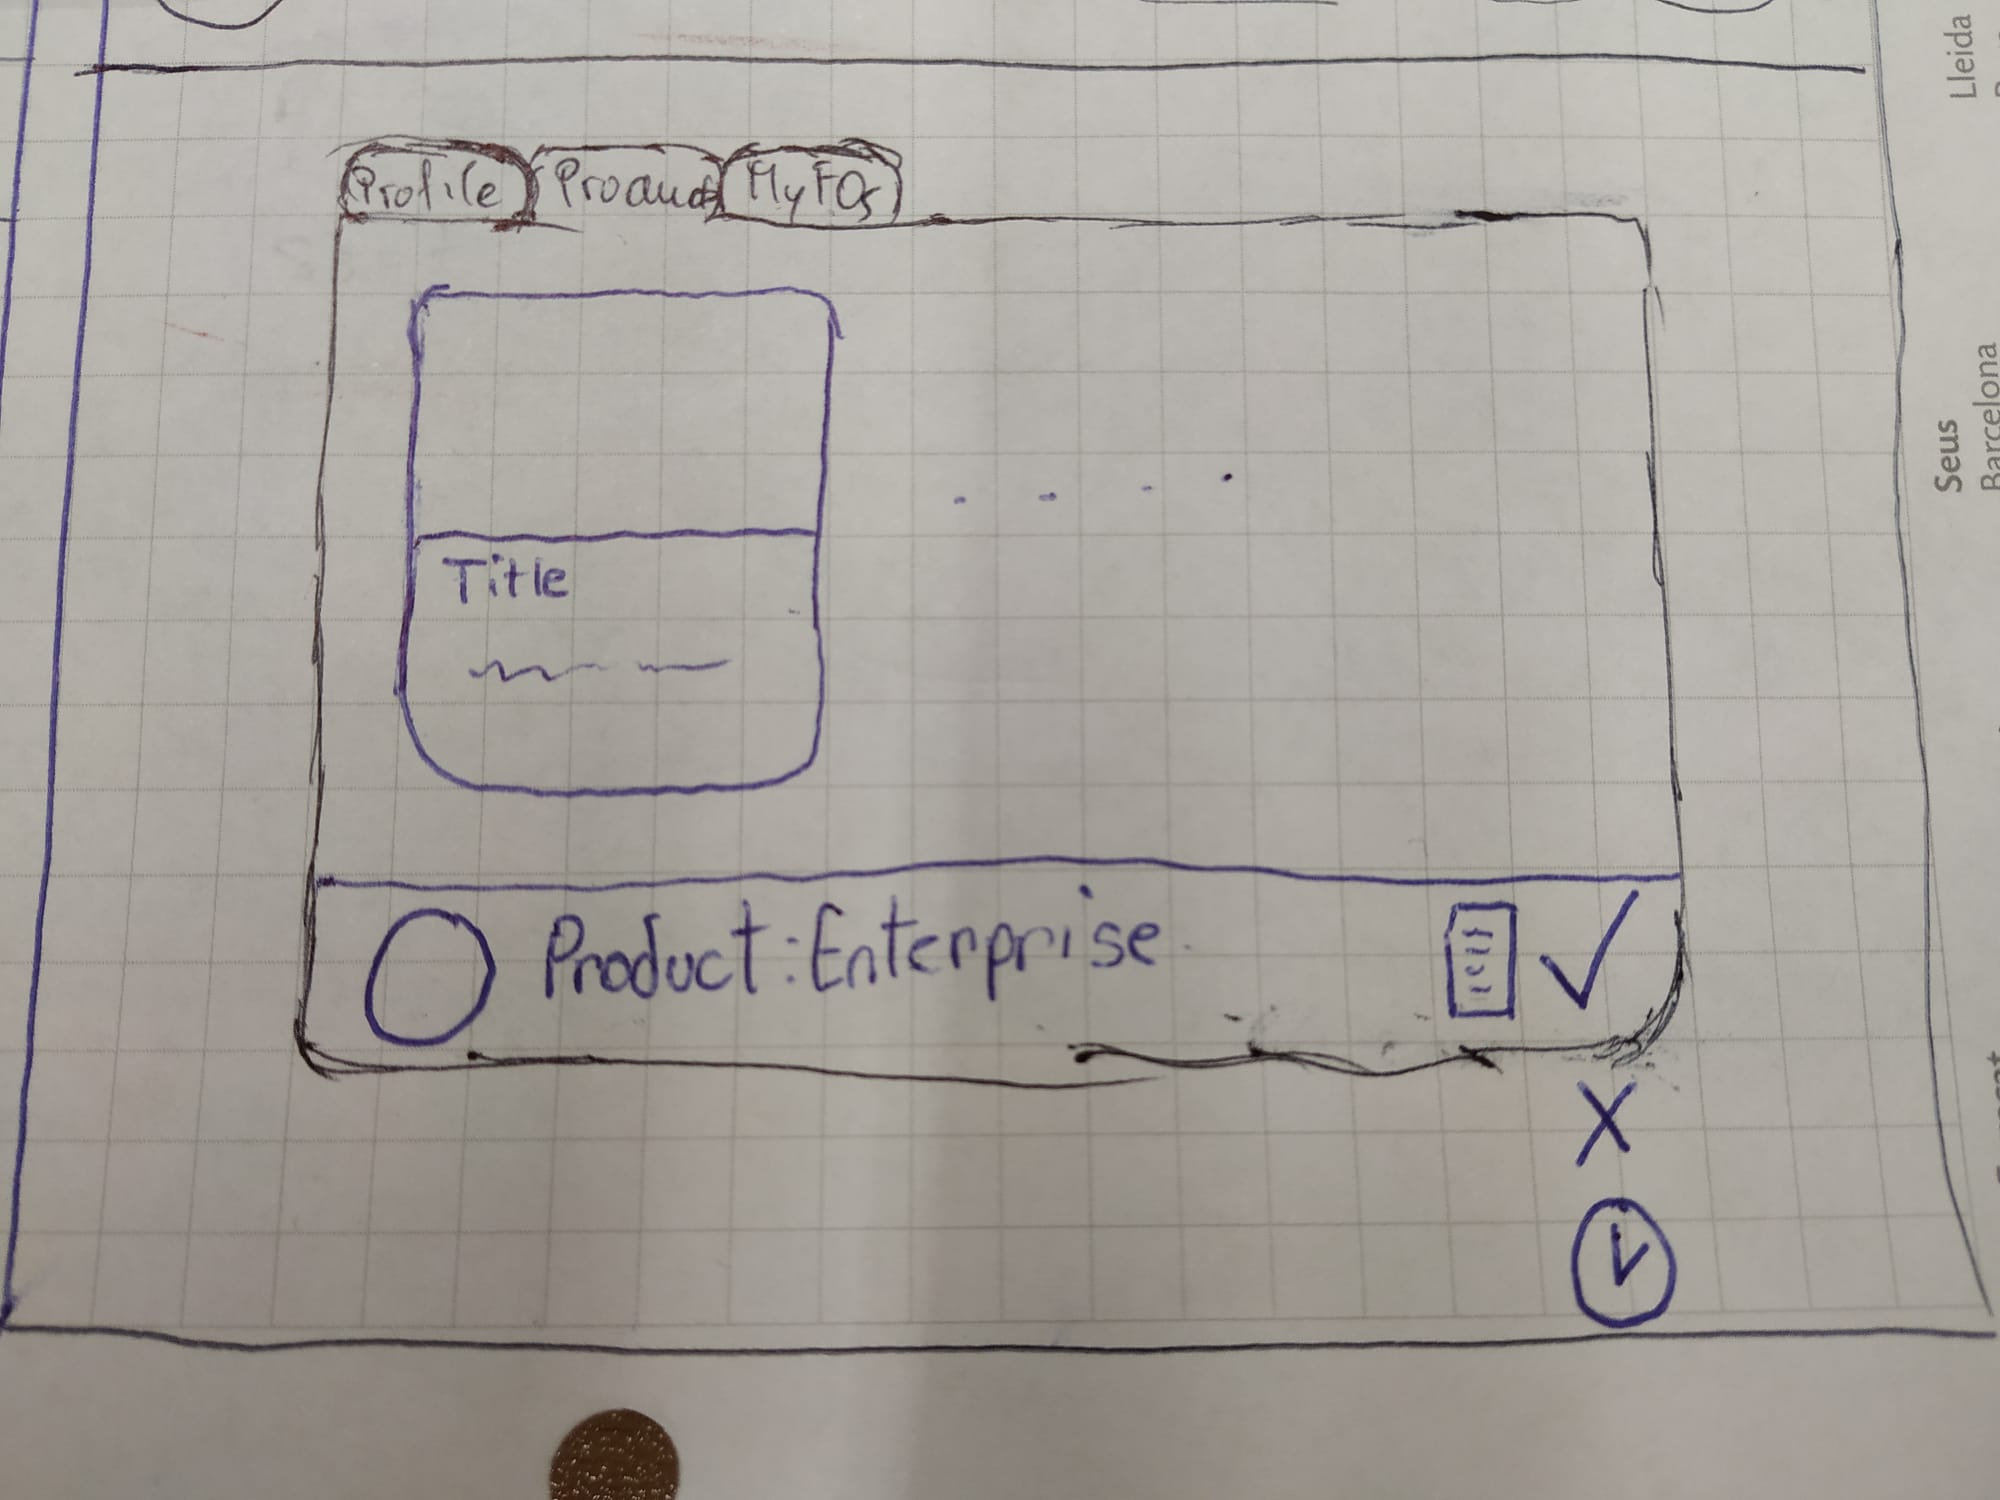
\includegraphics[width=0.5\linewidth]{img/webwire_3.jpeg}
  \caption{Products/Formal Offers Profile screen.}
  \label{fig:webwire-screen-1}
\end{figure}
\begin{figure}[H]
  \centering
  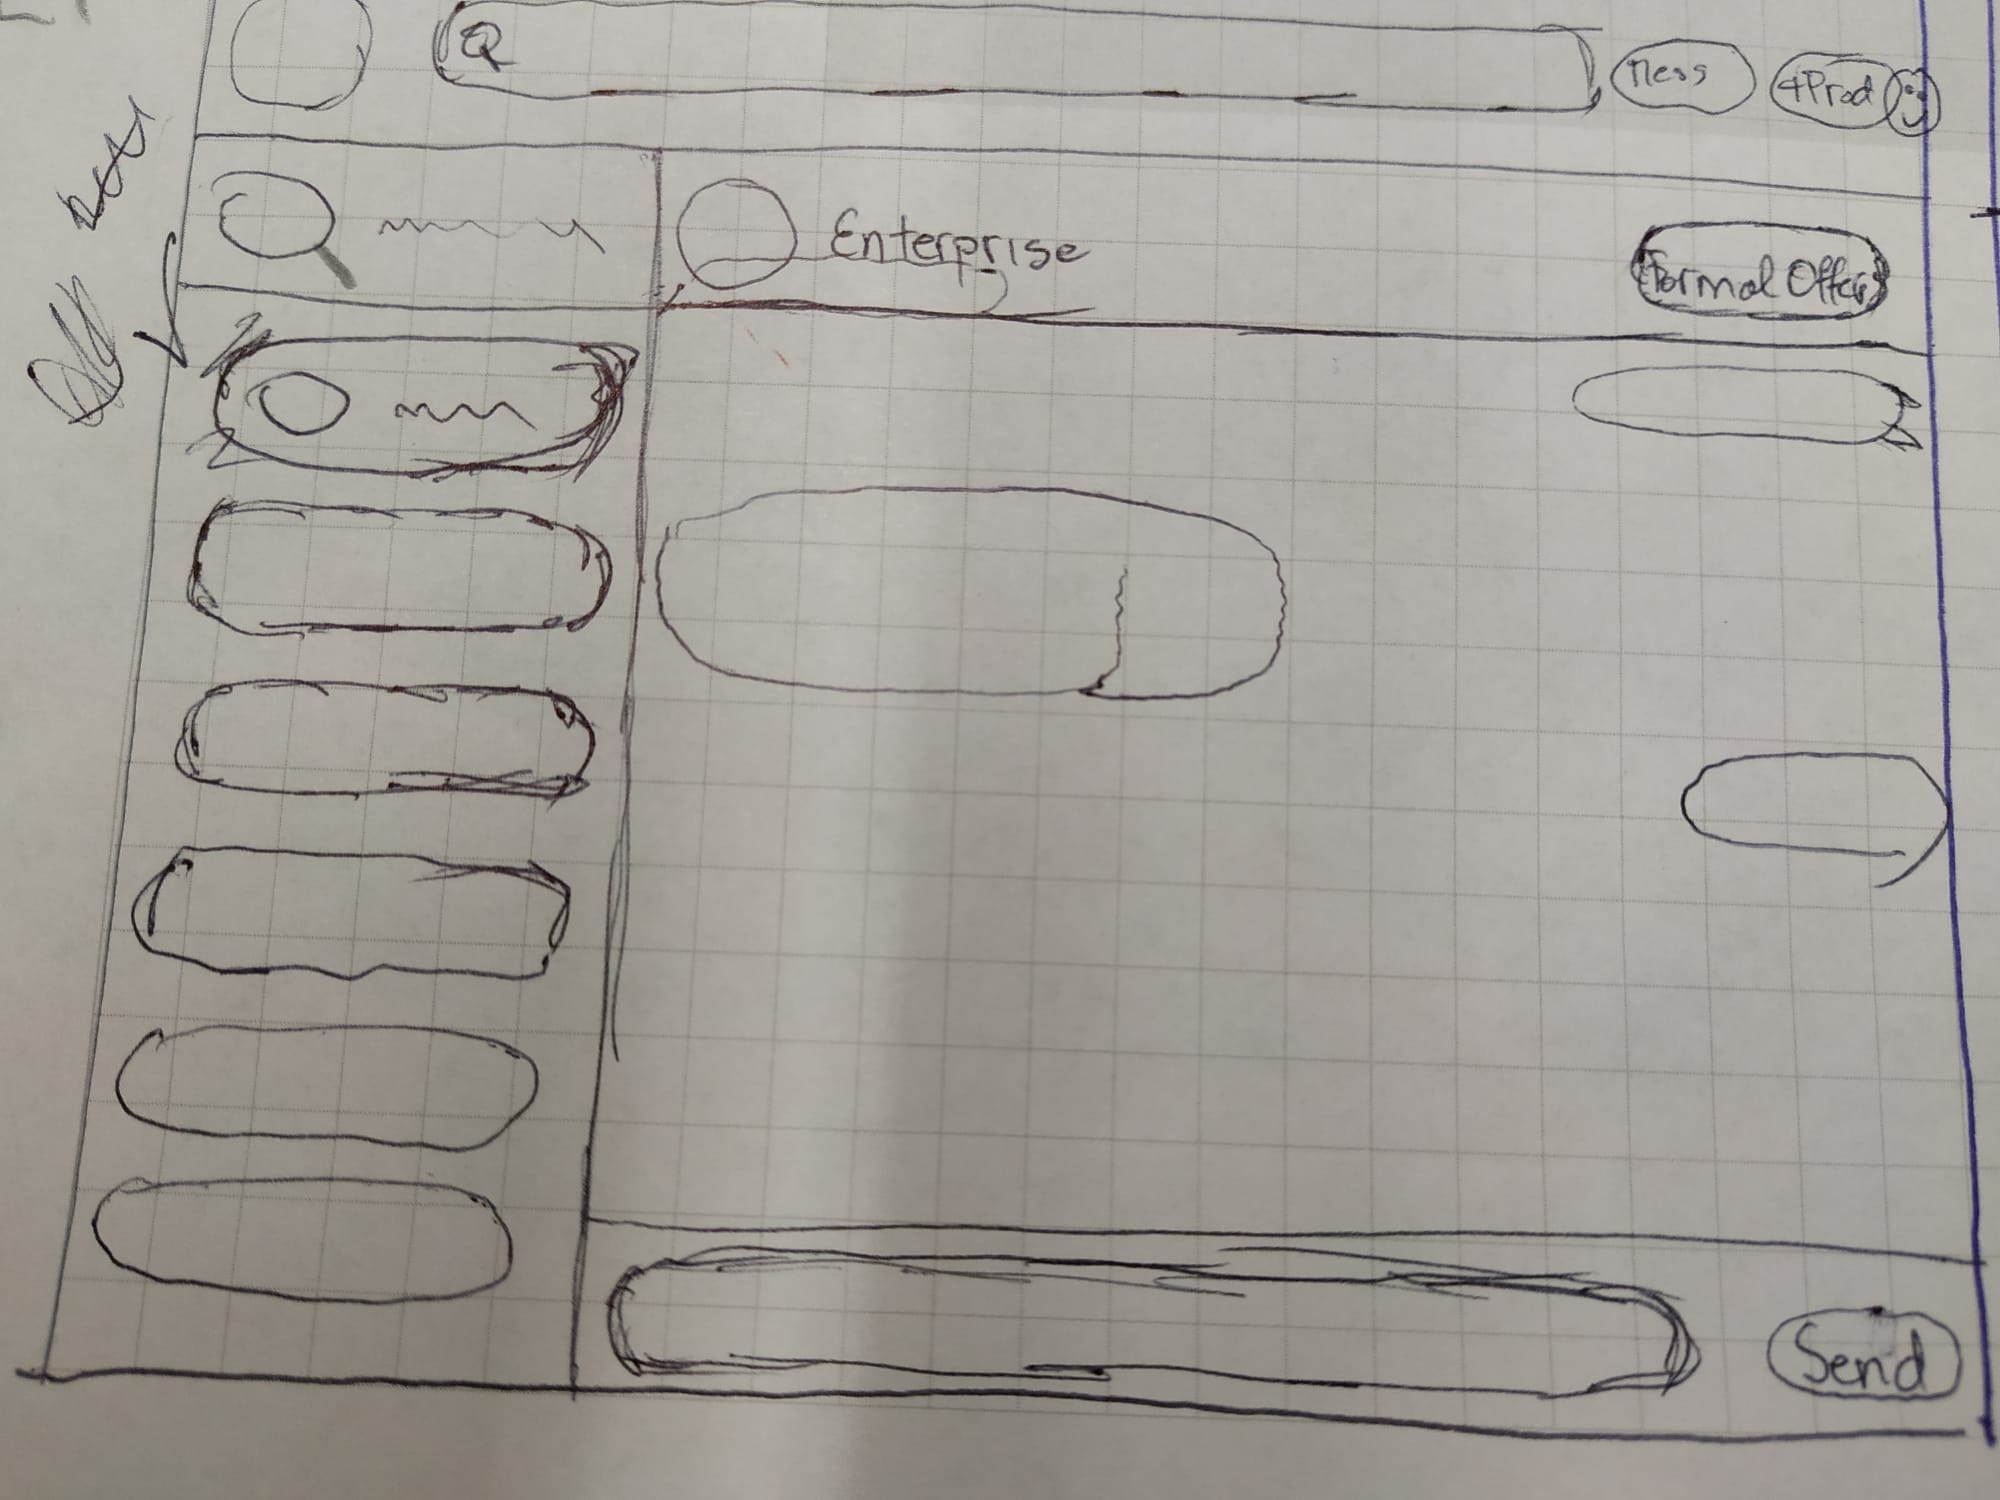
\includegraphics[width=0.5\linewidth]{img/webwire_4.jpeg}
  \caption{Chat screen.}
  \label{fig:webwire-screen-1}
\end{figure}
\begin{figure}[H]
  \centering
  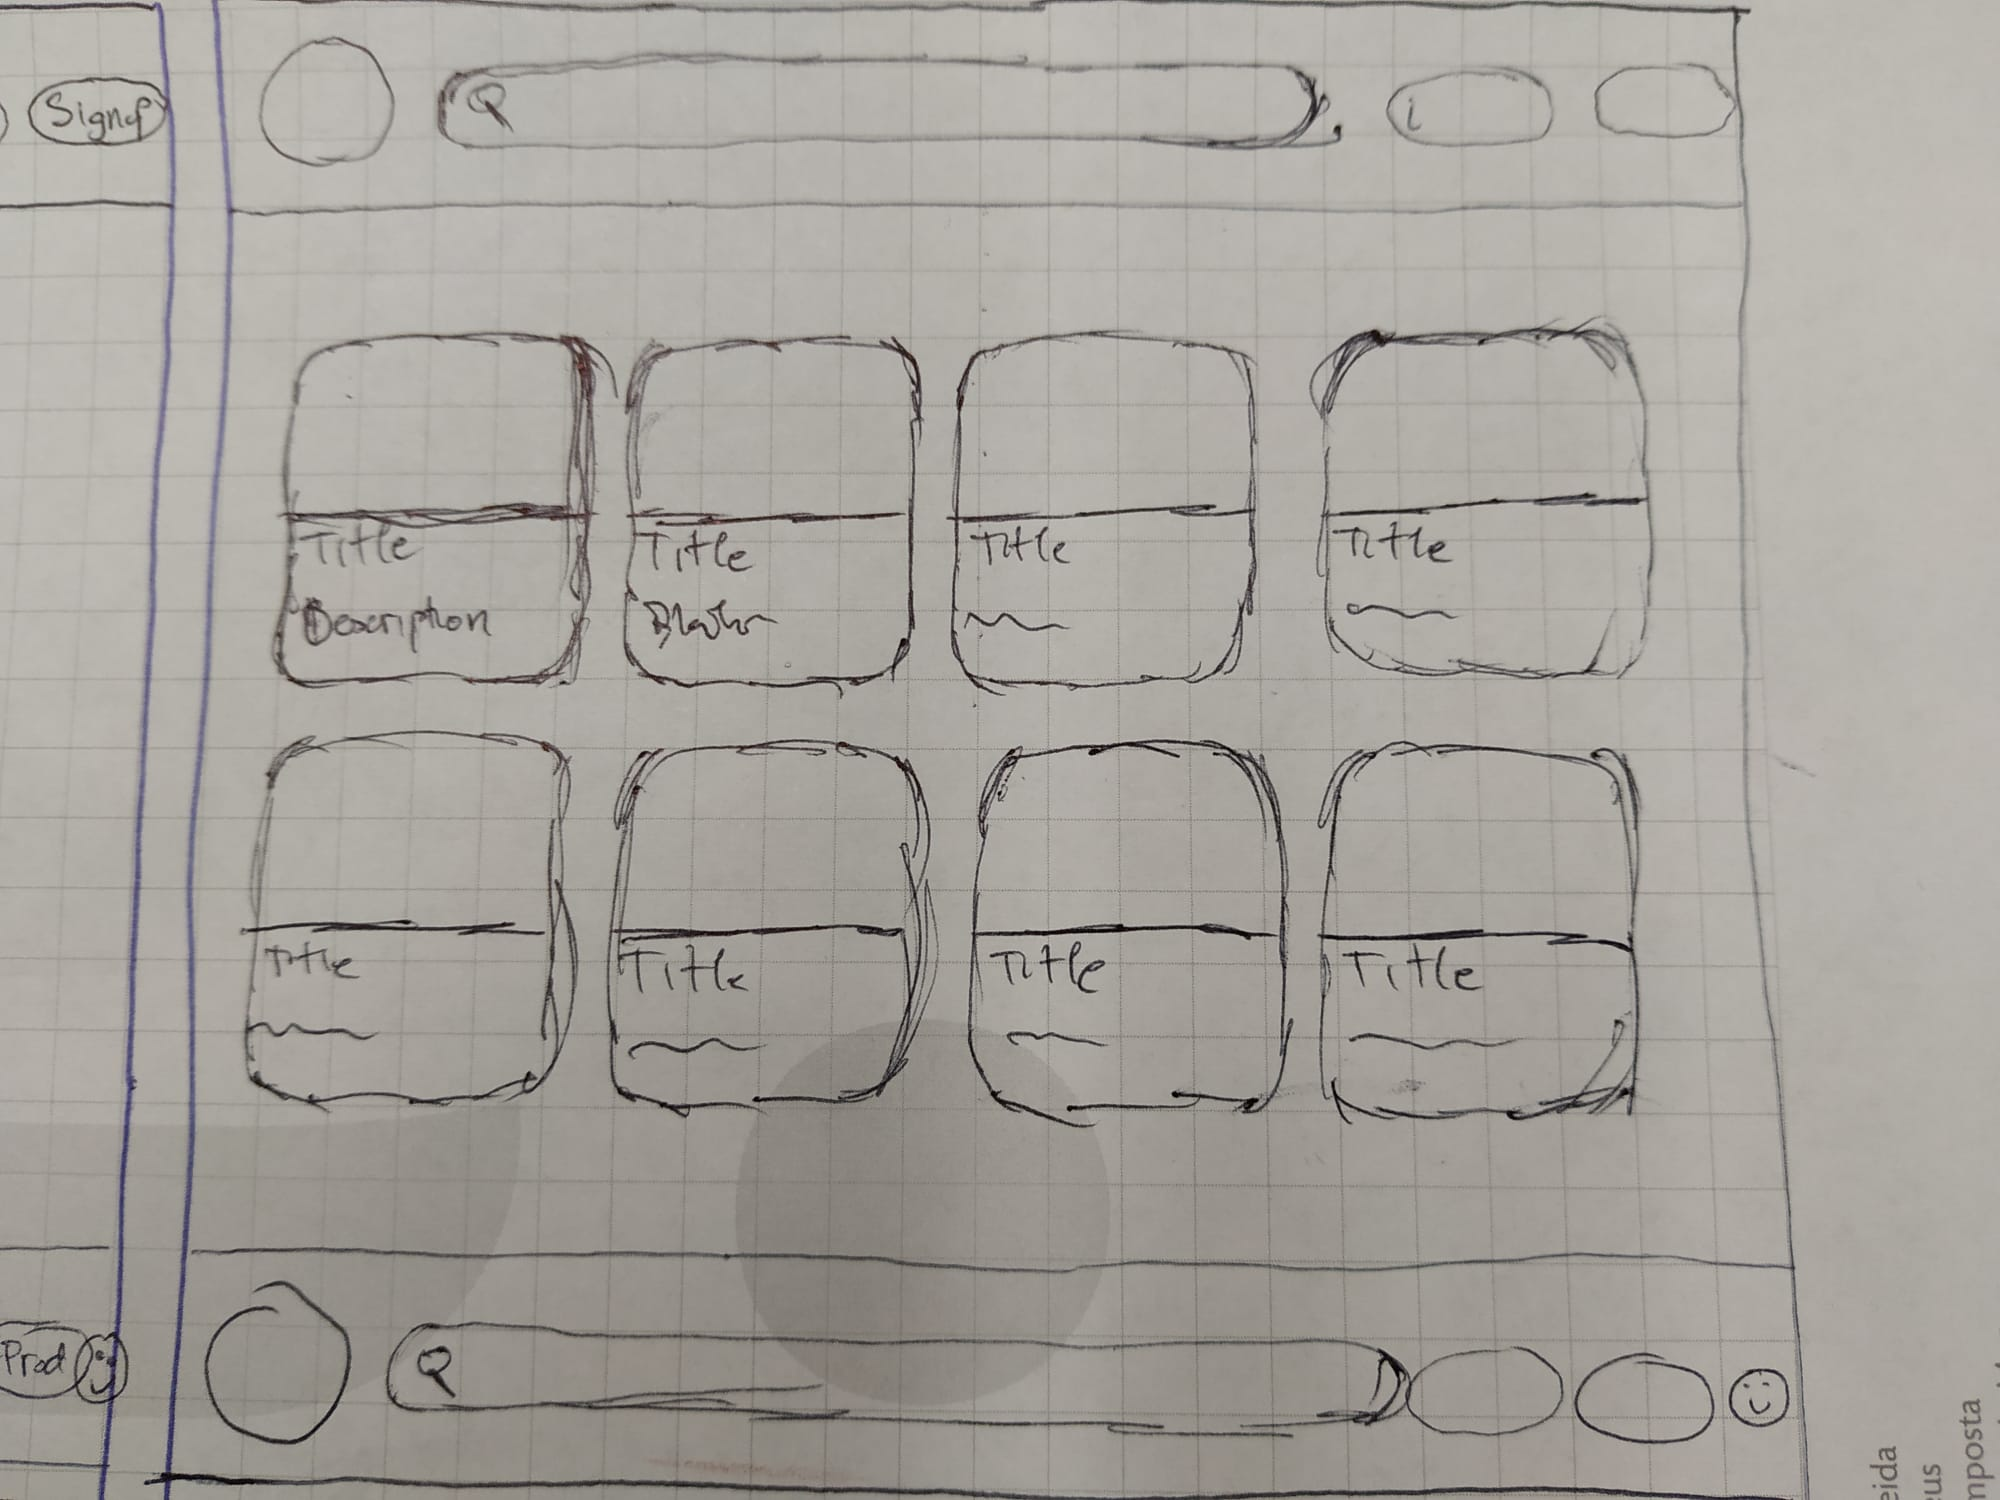
\includegraphics[width=0.5\linewidth]{img/webwire_5.jpeg}
  \caption{Search screen.}
  \label{fig:webwire-screen-1}
\end{figure}
\begin{figure}[H]
  \centering
  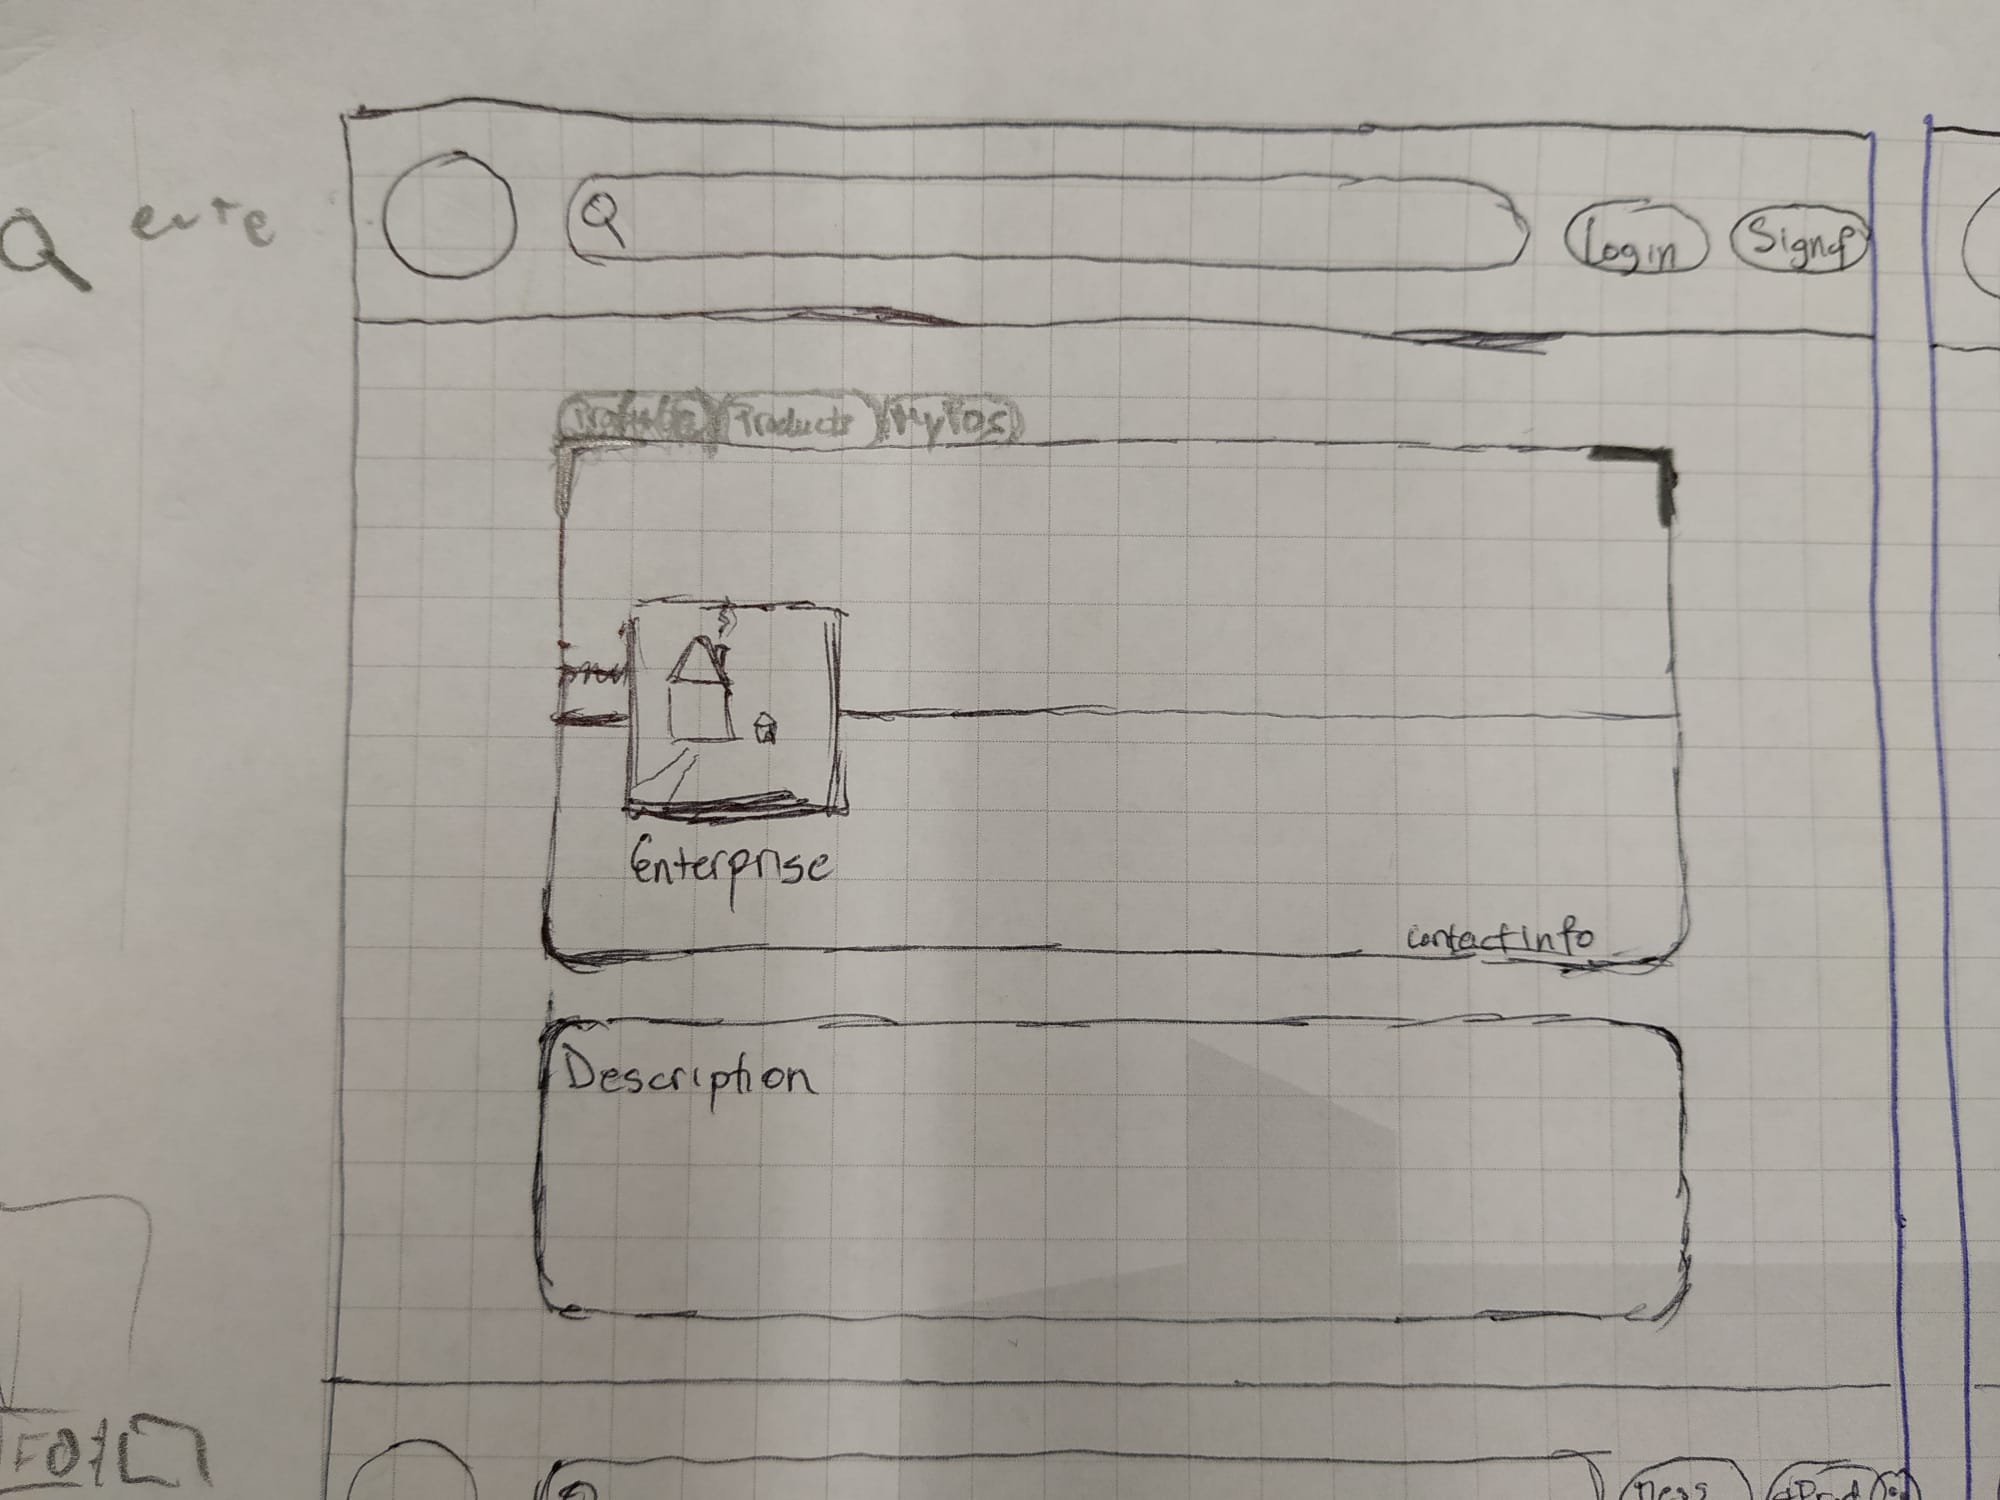
\includegraphics[width=0.5\linewidth]{img/webwire_6.jpeg}
  \caption{Profile screen.}
  \label{fig:webwire-screen-1}
\end{figure}
\begin{figure}[H]
  \centering
  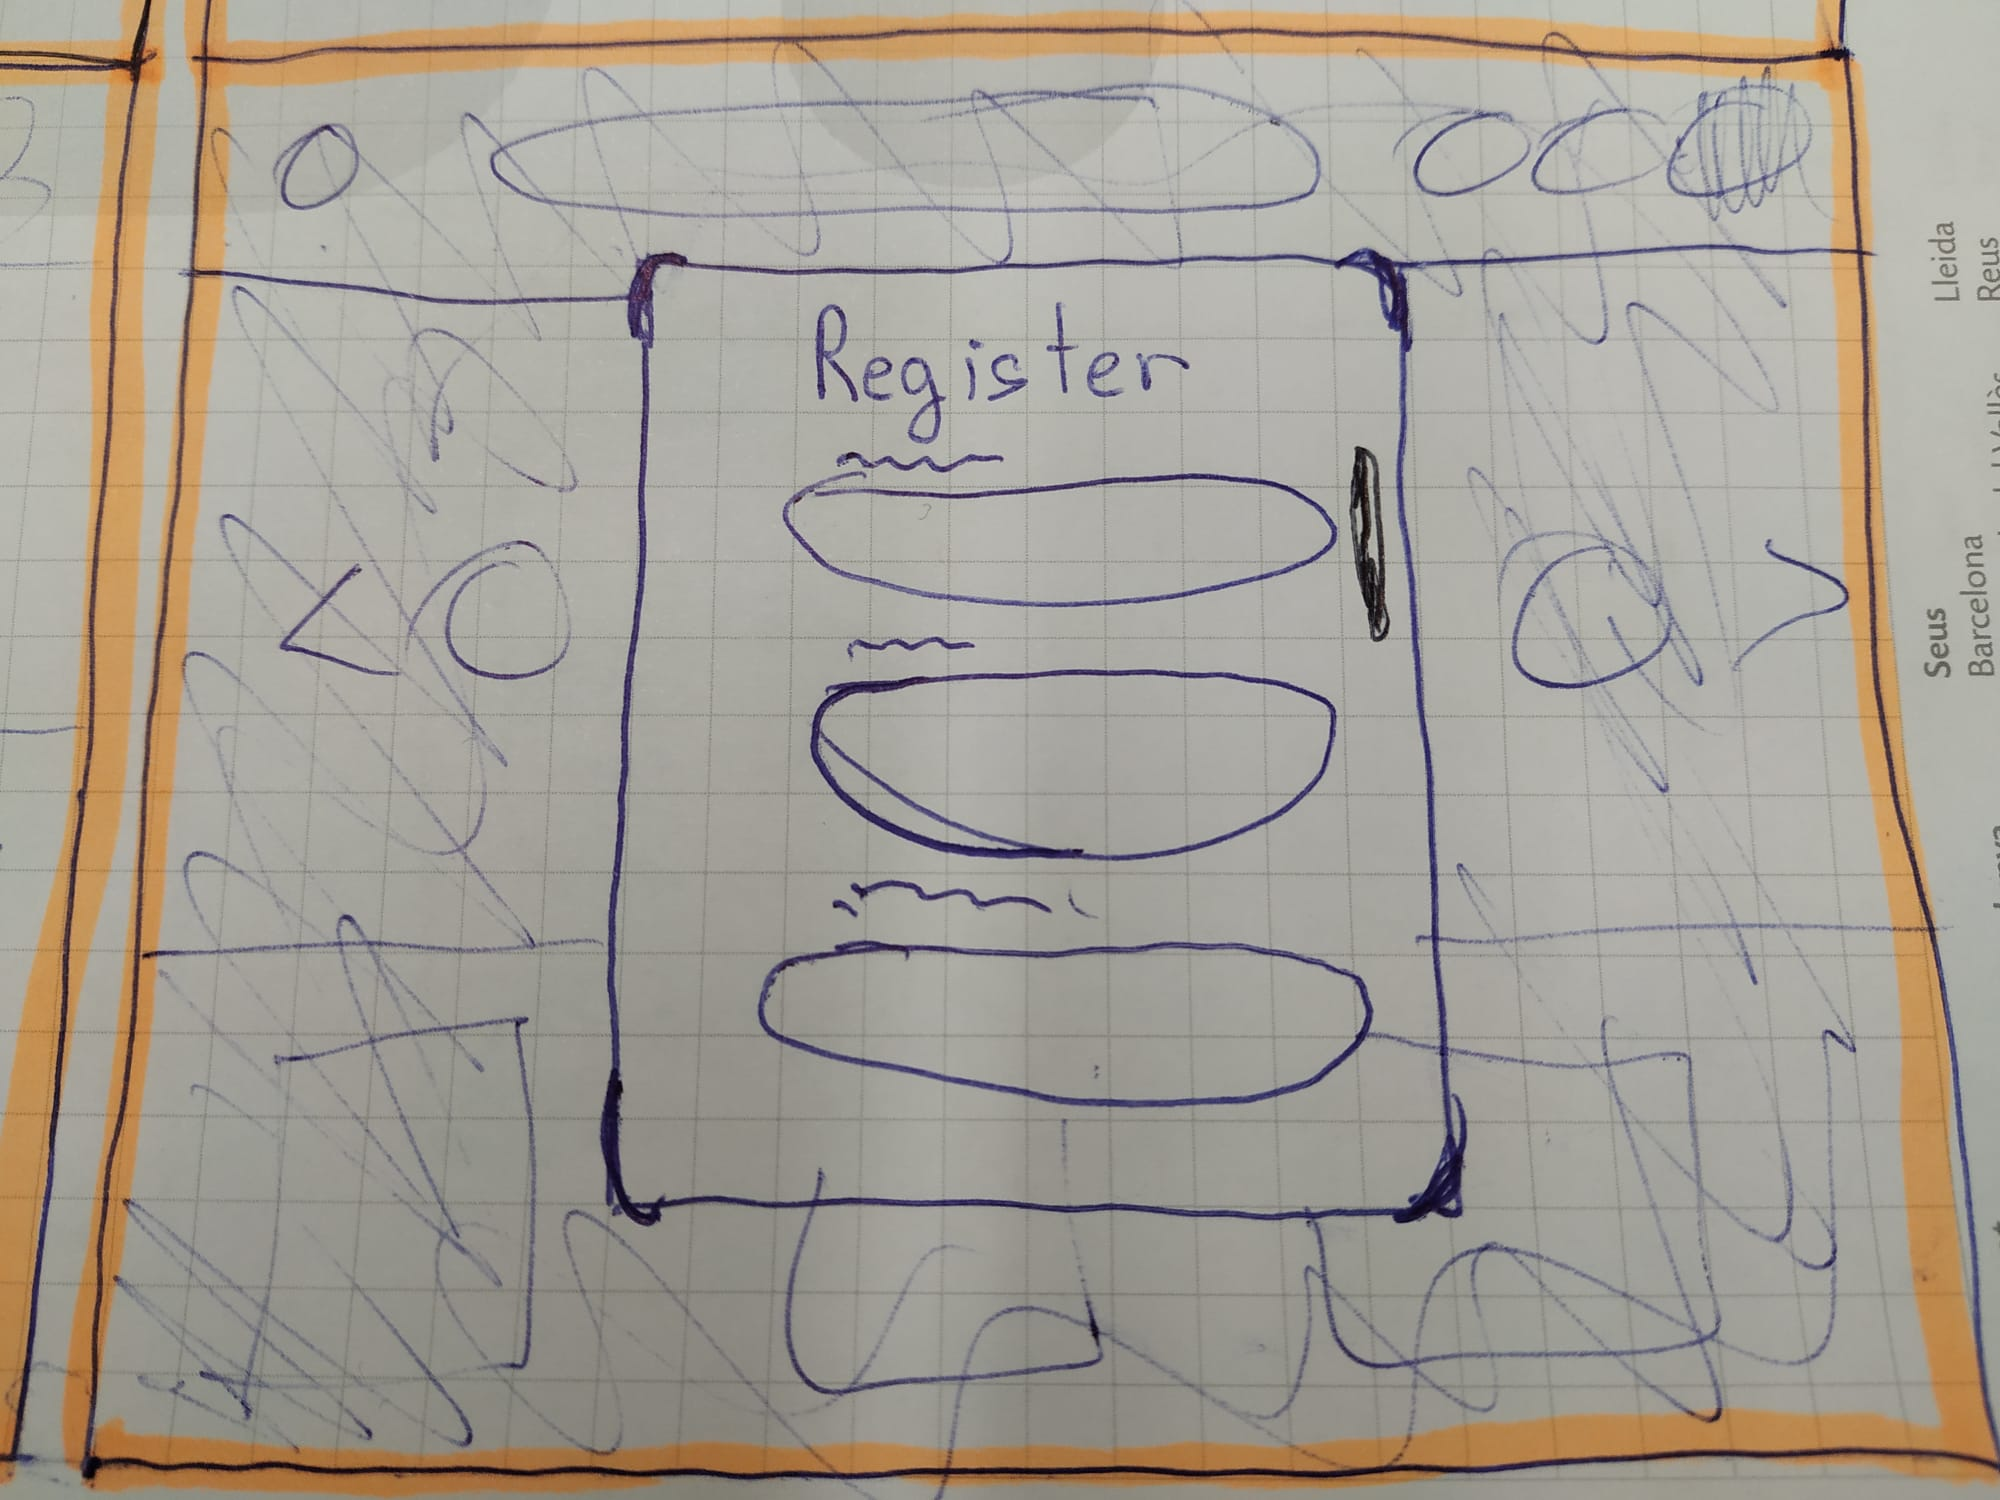
\includegraphics[width=0.5\linewidth]{img/webwire_7.jpeg}
  \caption{Register screen.}
  \label{fig:webwire-screen-1}
\end{figure}
\begin{figure}[H]
  \centering
  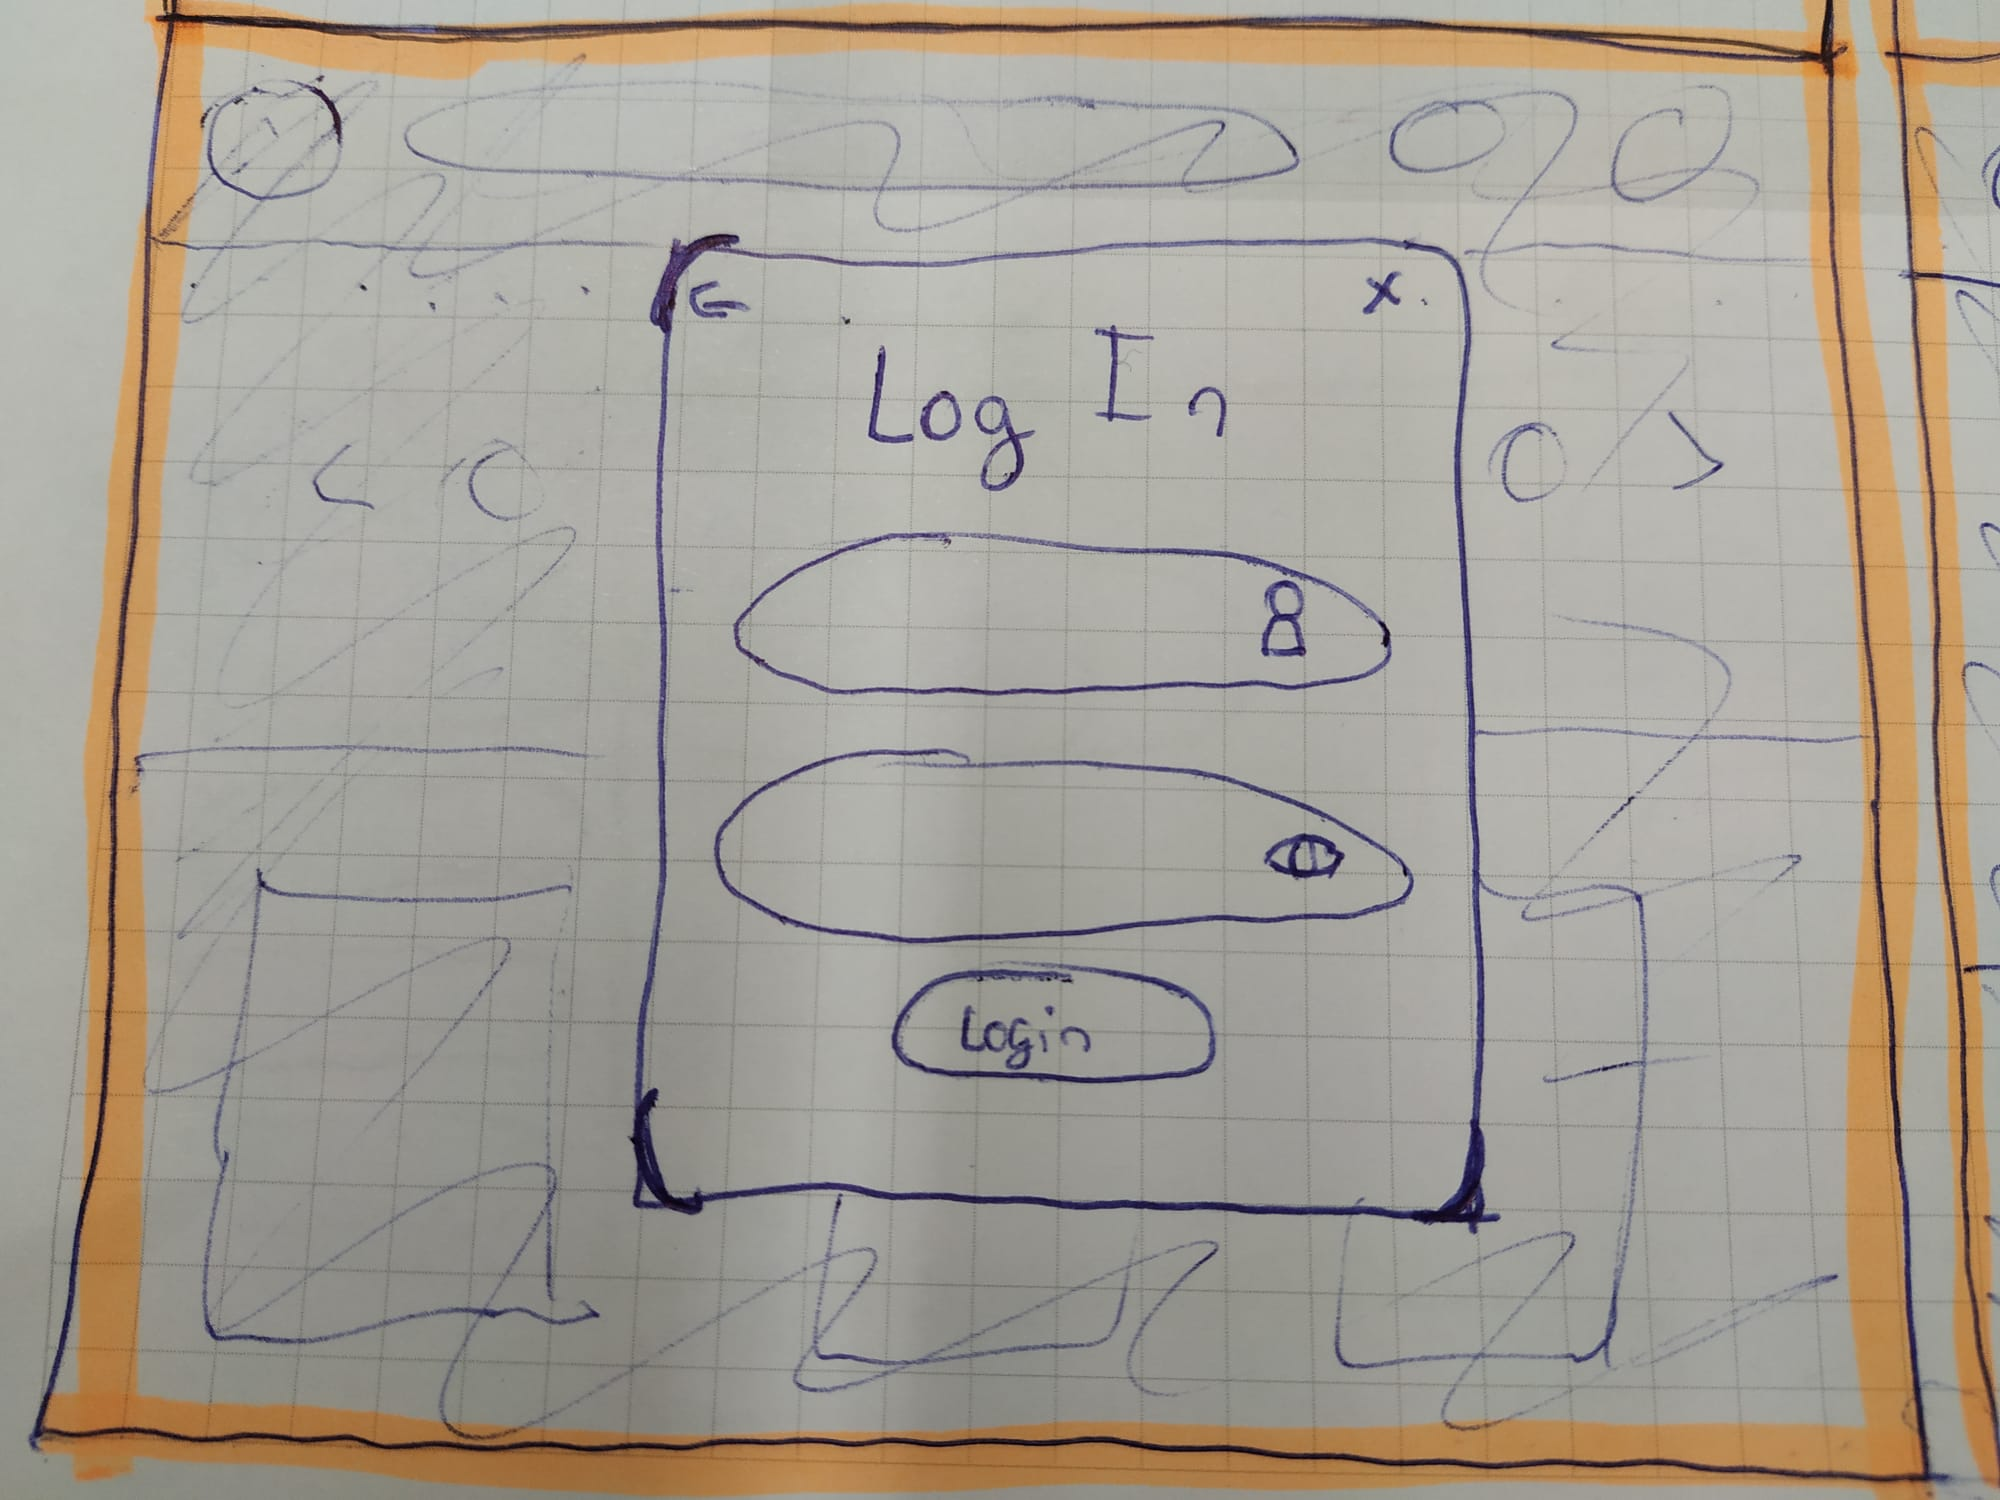
\includegraphics[width=0.5\linewidth]{img/webwire_8.jpeg}
  \caption{Log In screen.}
  \label{fig:webwire-screen-1}
\end{figure}
\begin{figure}[H]
  \centering
  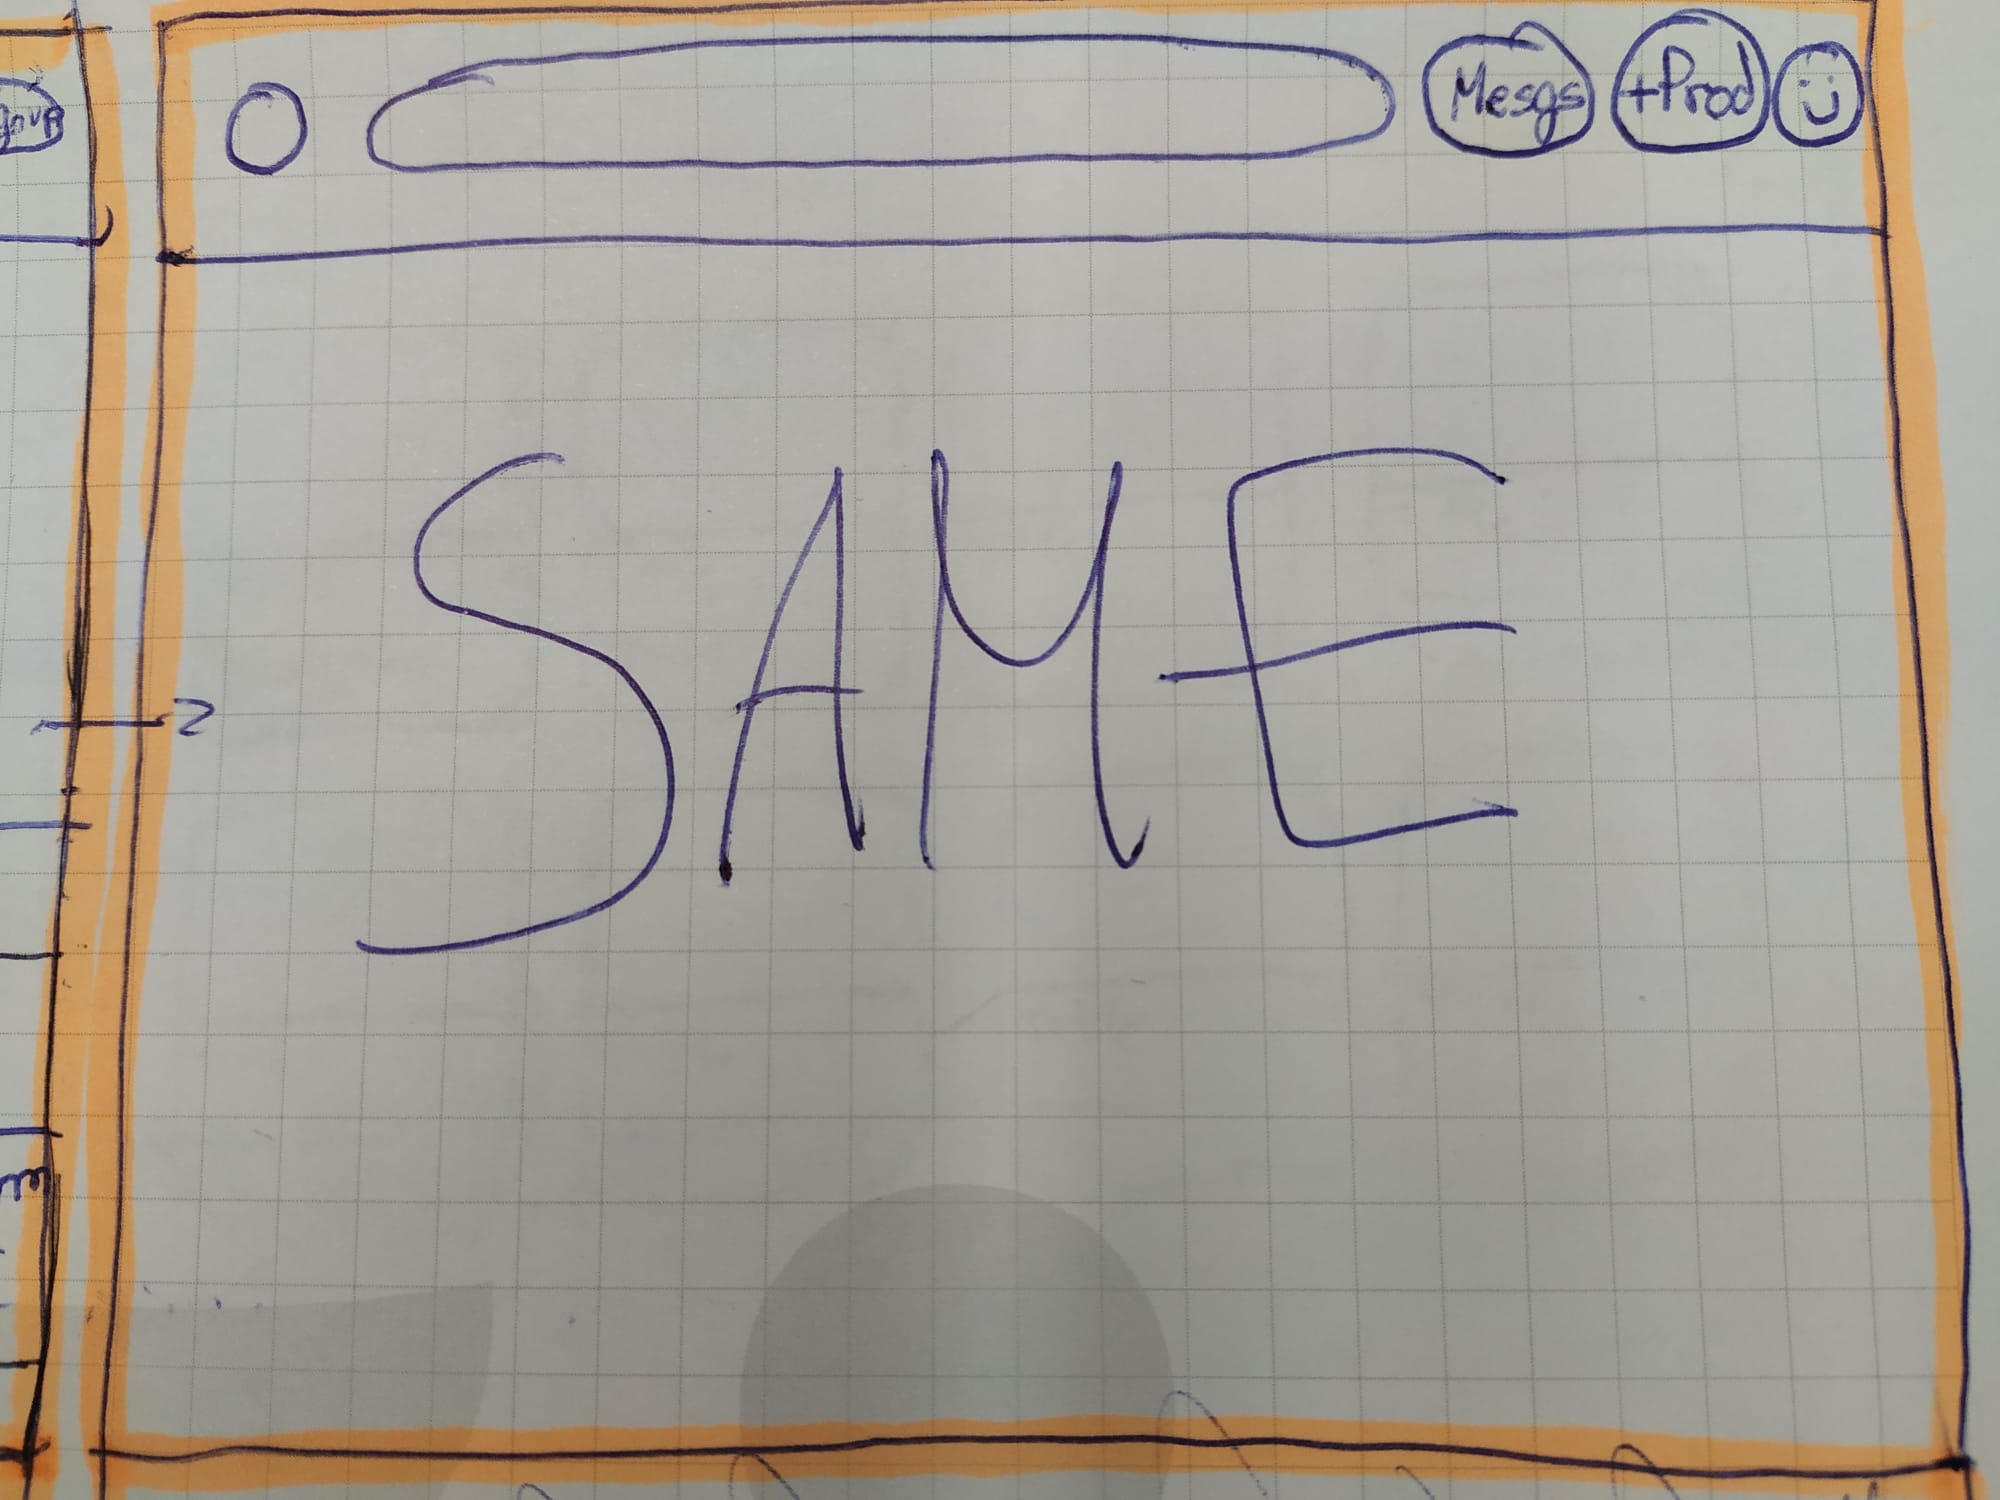
\includegraphics[width=0.5\linewidth]{img/webwire_9.jpeg}
  \caption{Home Loged In screen.}
  \label{fig:webwire-screen-1}
\end{figure}
\begin{figure}[H]
  \centering
  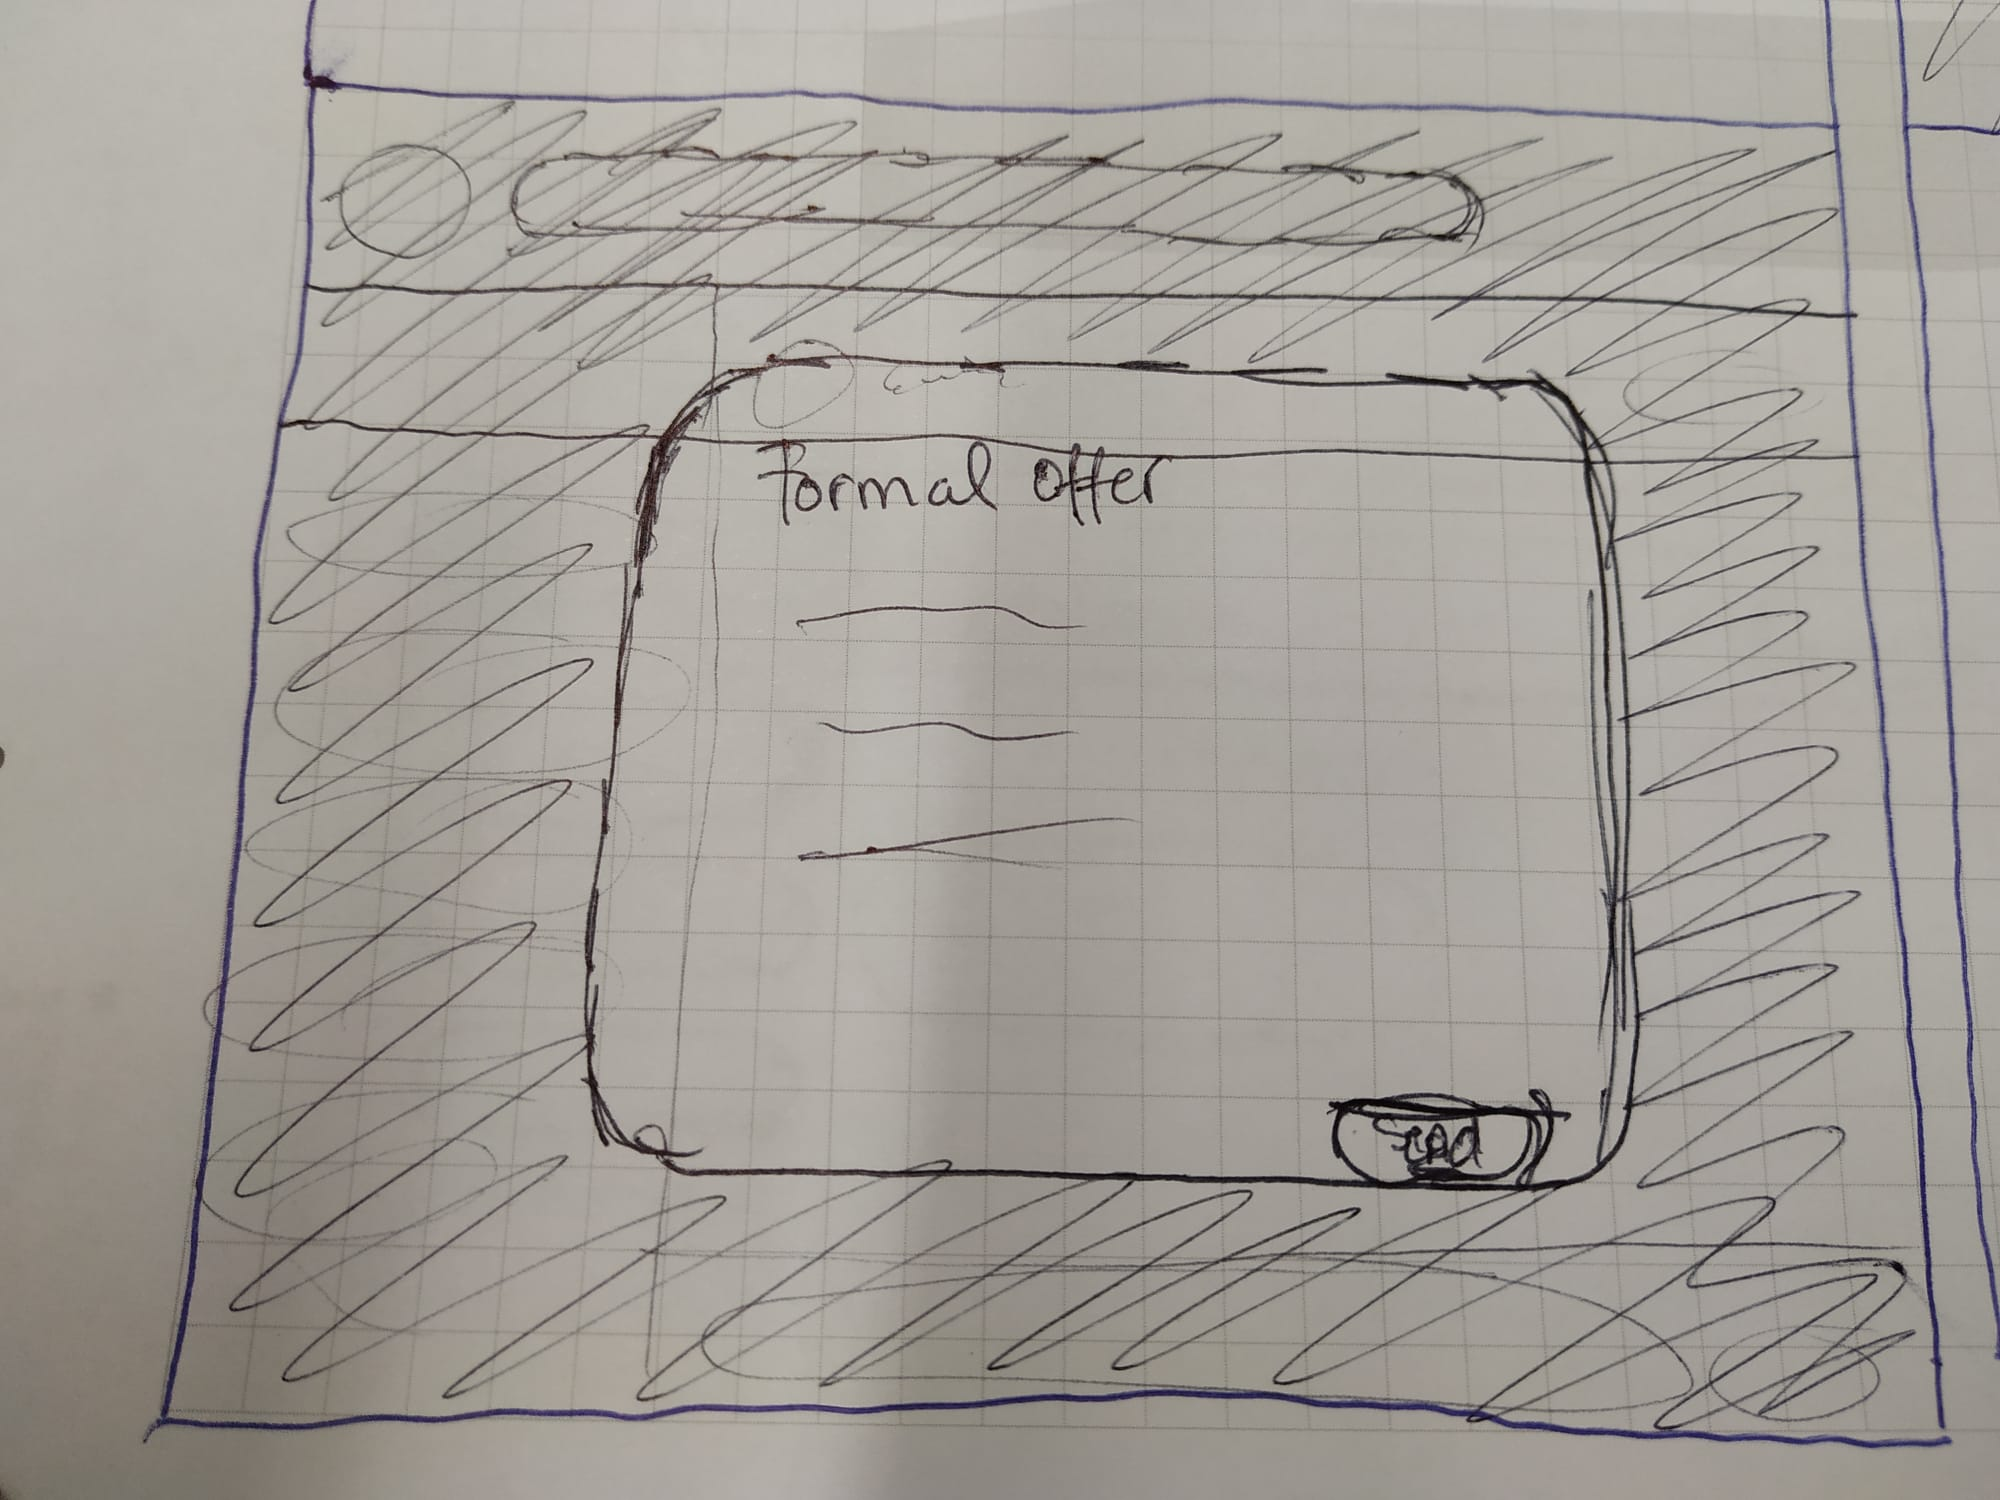
\includegraphics[width=0.5\linewidth]{img/webwire_10.jpeg}
  \caption{Formal Offer Send screen.}
  \label{fig:webwire-screen-1}
\end{figure}
\begin{figure}[H]
  \centering
  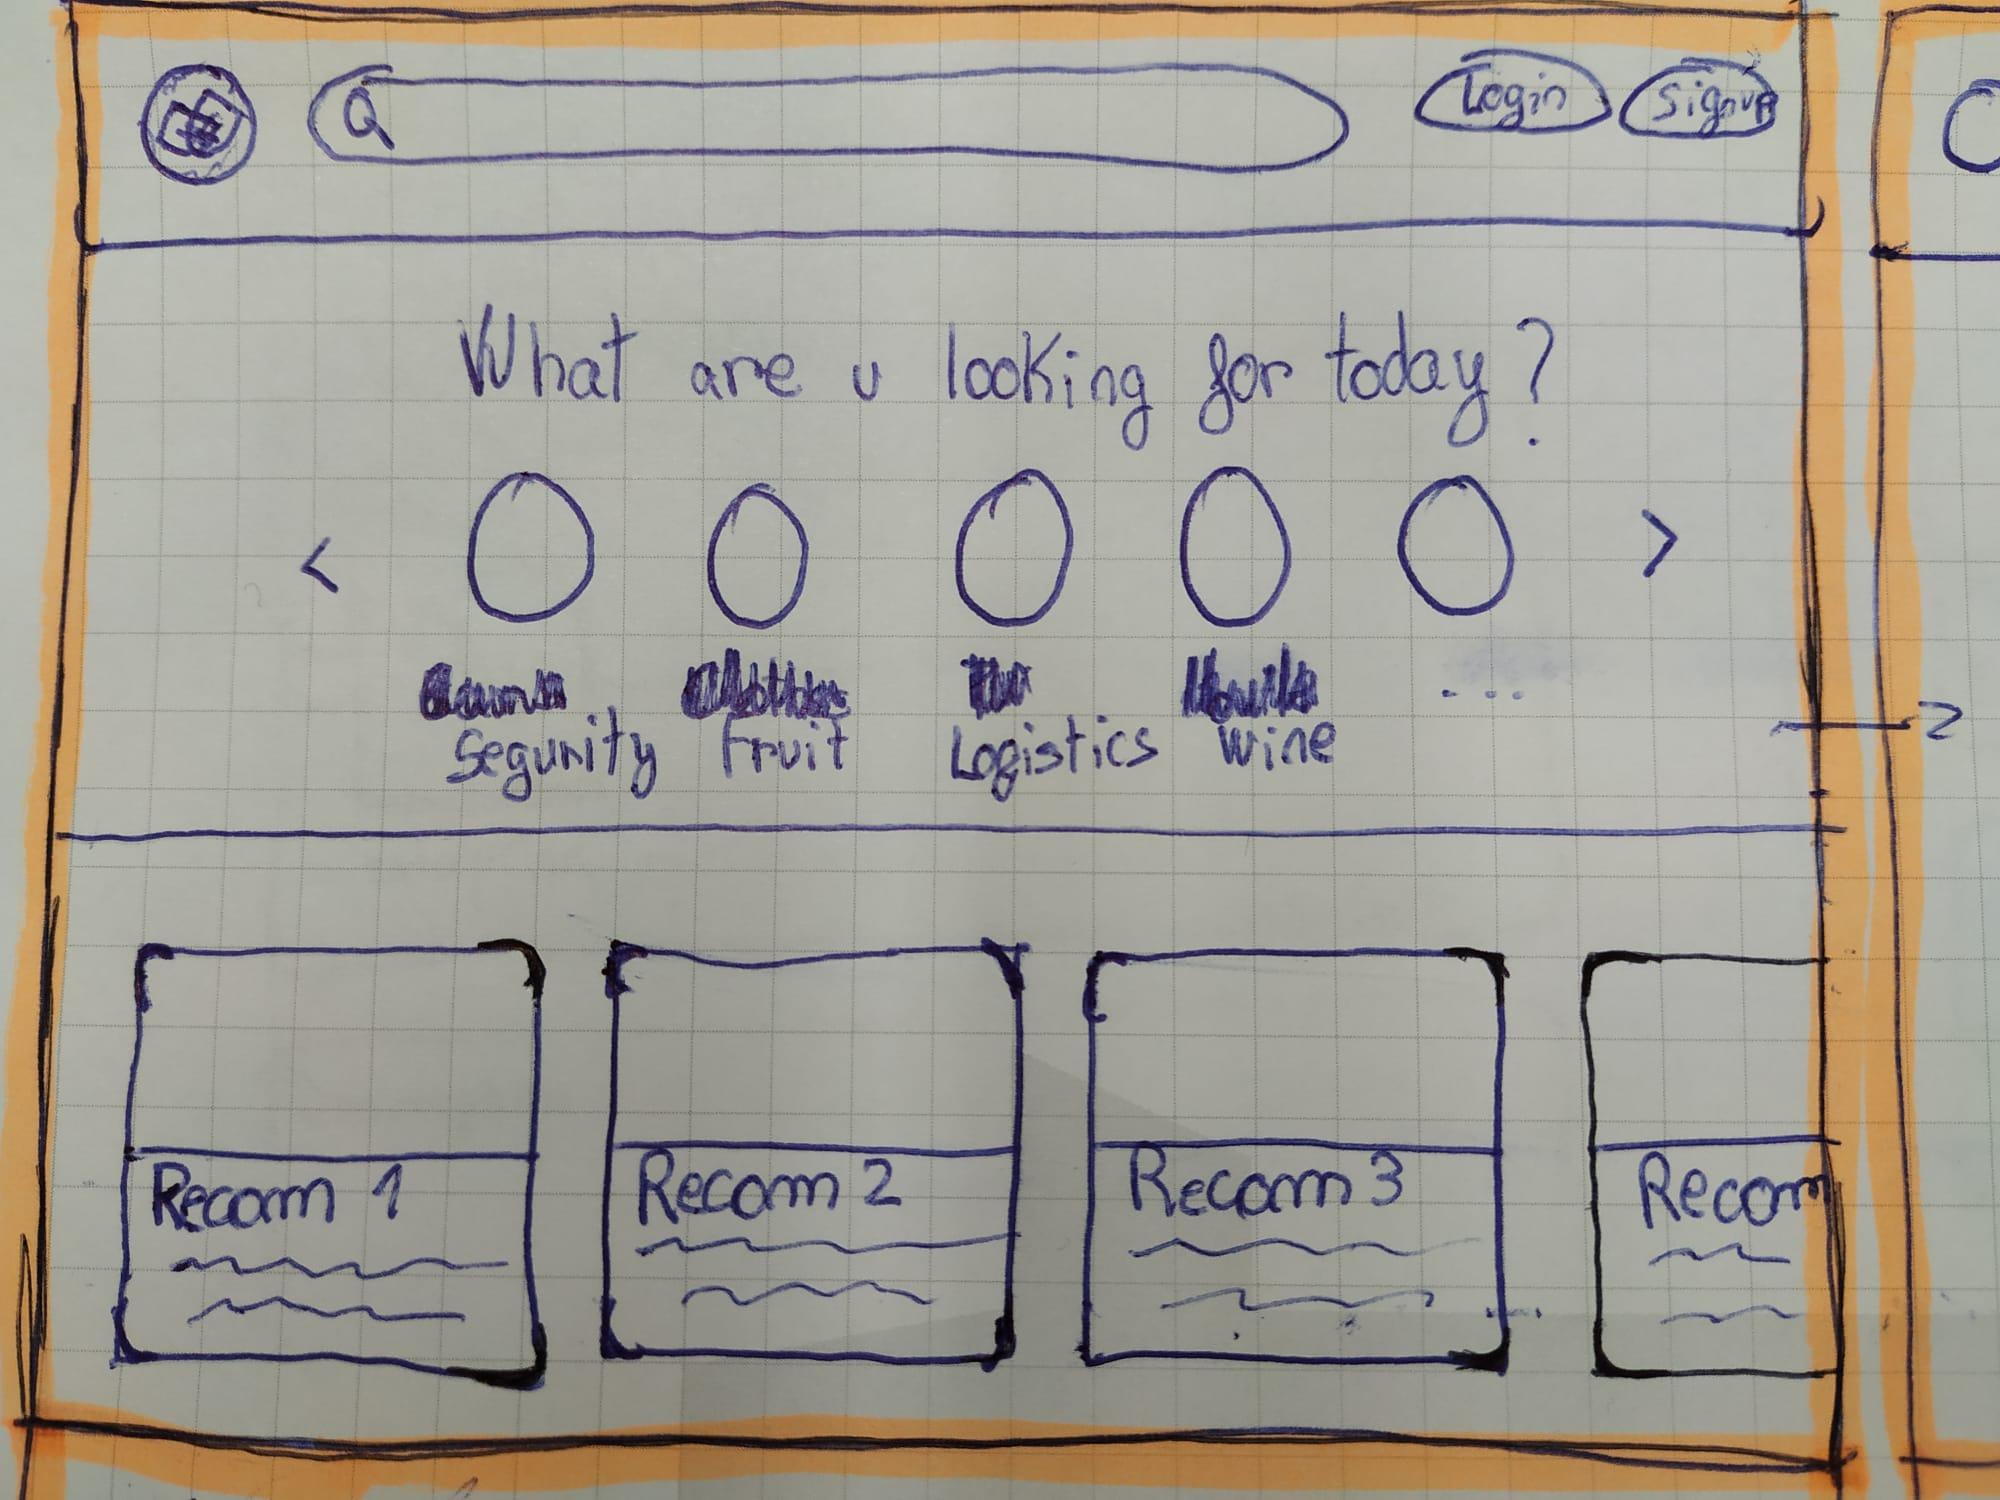
\includegraphics[width=0.5\linewidth]{img/webwire_11.jpeg}
  \caption{Home screen.}
  \label{fig:webwire-screen-1}
\end{figure}

\subsubsection{Application}
In this section we are going to show all the Screens that are actually in our application.
\begin{figure}[H]
  \centering
  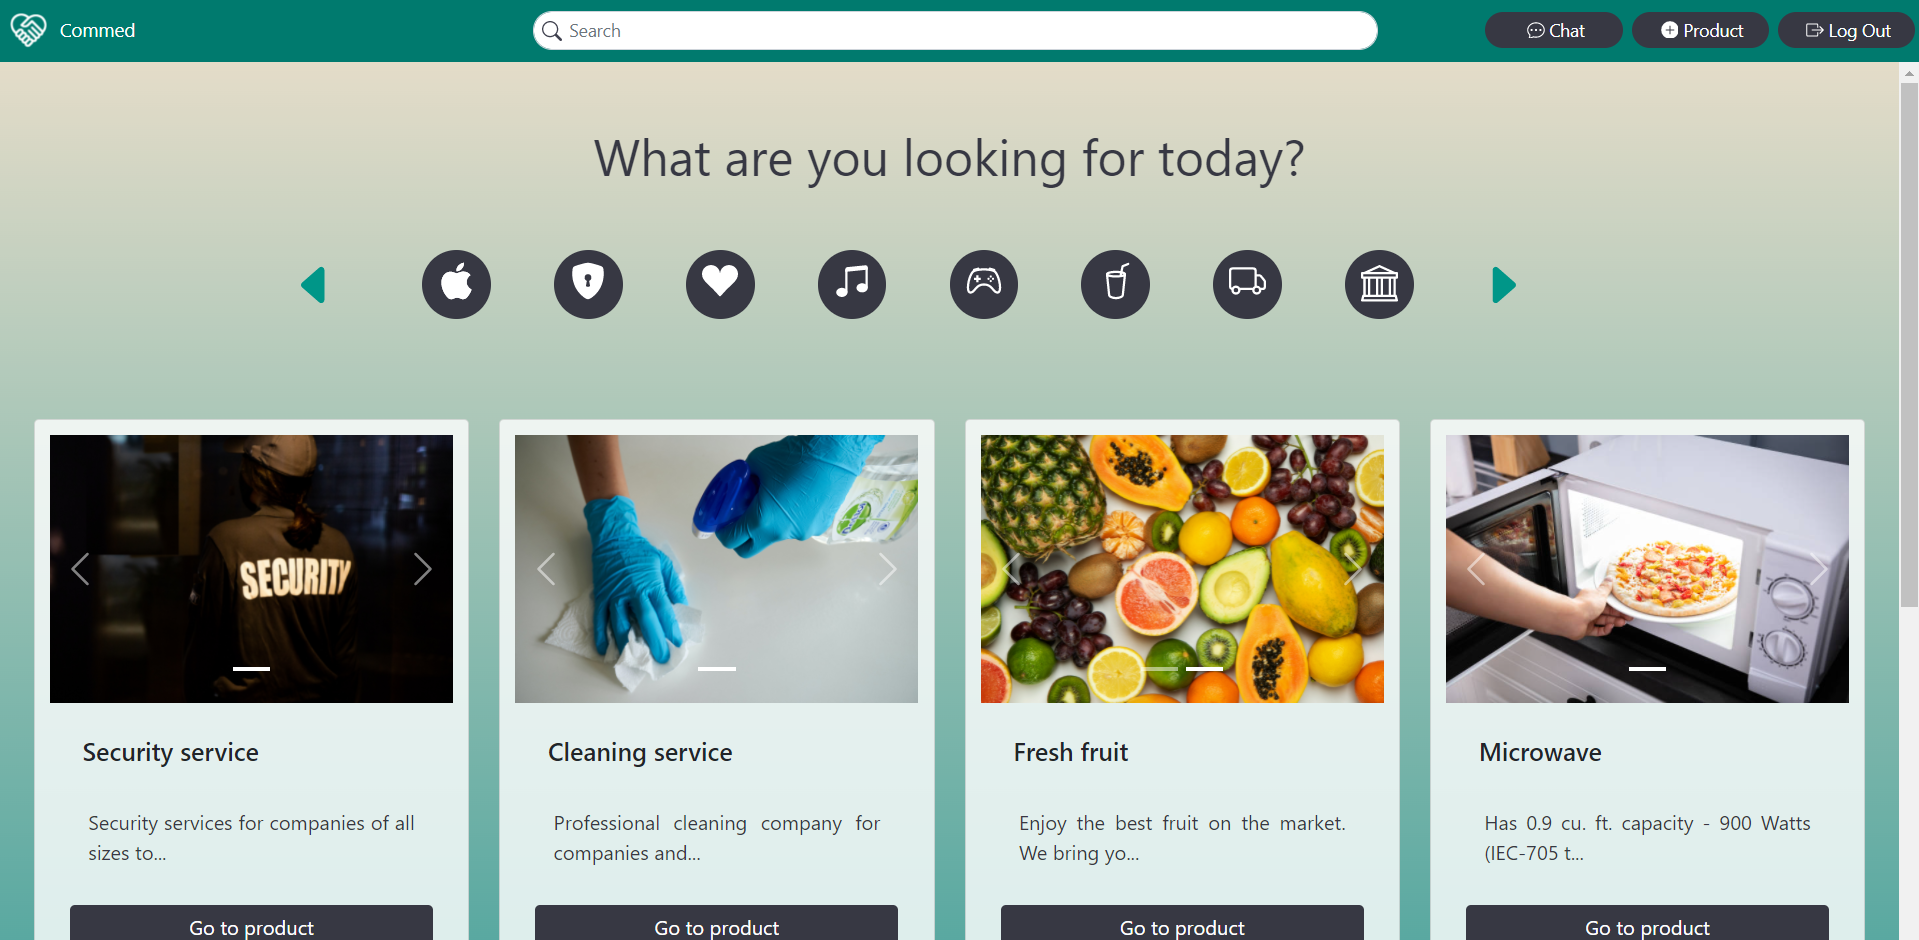
\includegraphics[width=0.5\linewidth]{img/webclient_2.png}
  \caption{Home screen.}
  \label{fig:webclient-screen-1}
\end{figure}
\begin{figure}[H]
  \centering
  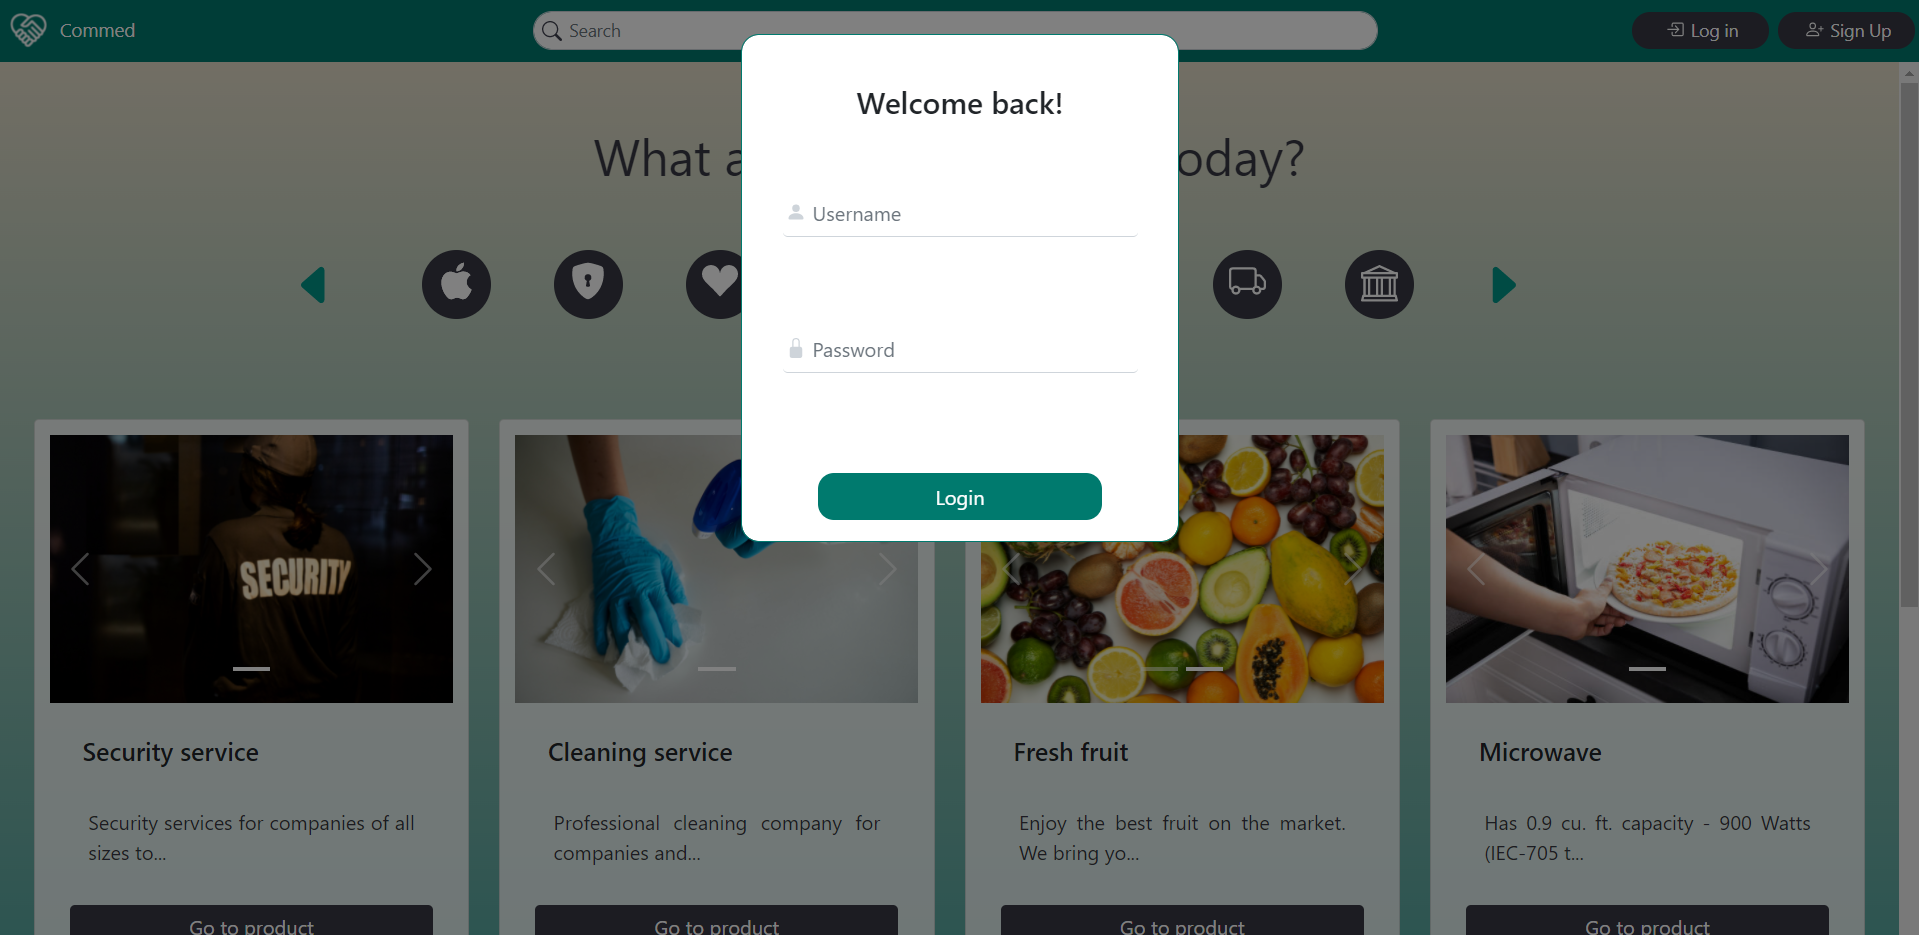
\includegraphics[width=0.5\linewidth]{img/webclient_3.png}
  \caption{Log In screen.}
  \label{fig:webclient-screen-2}
\end{figure}
\begin{figure}[H]
  \centering
  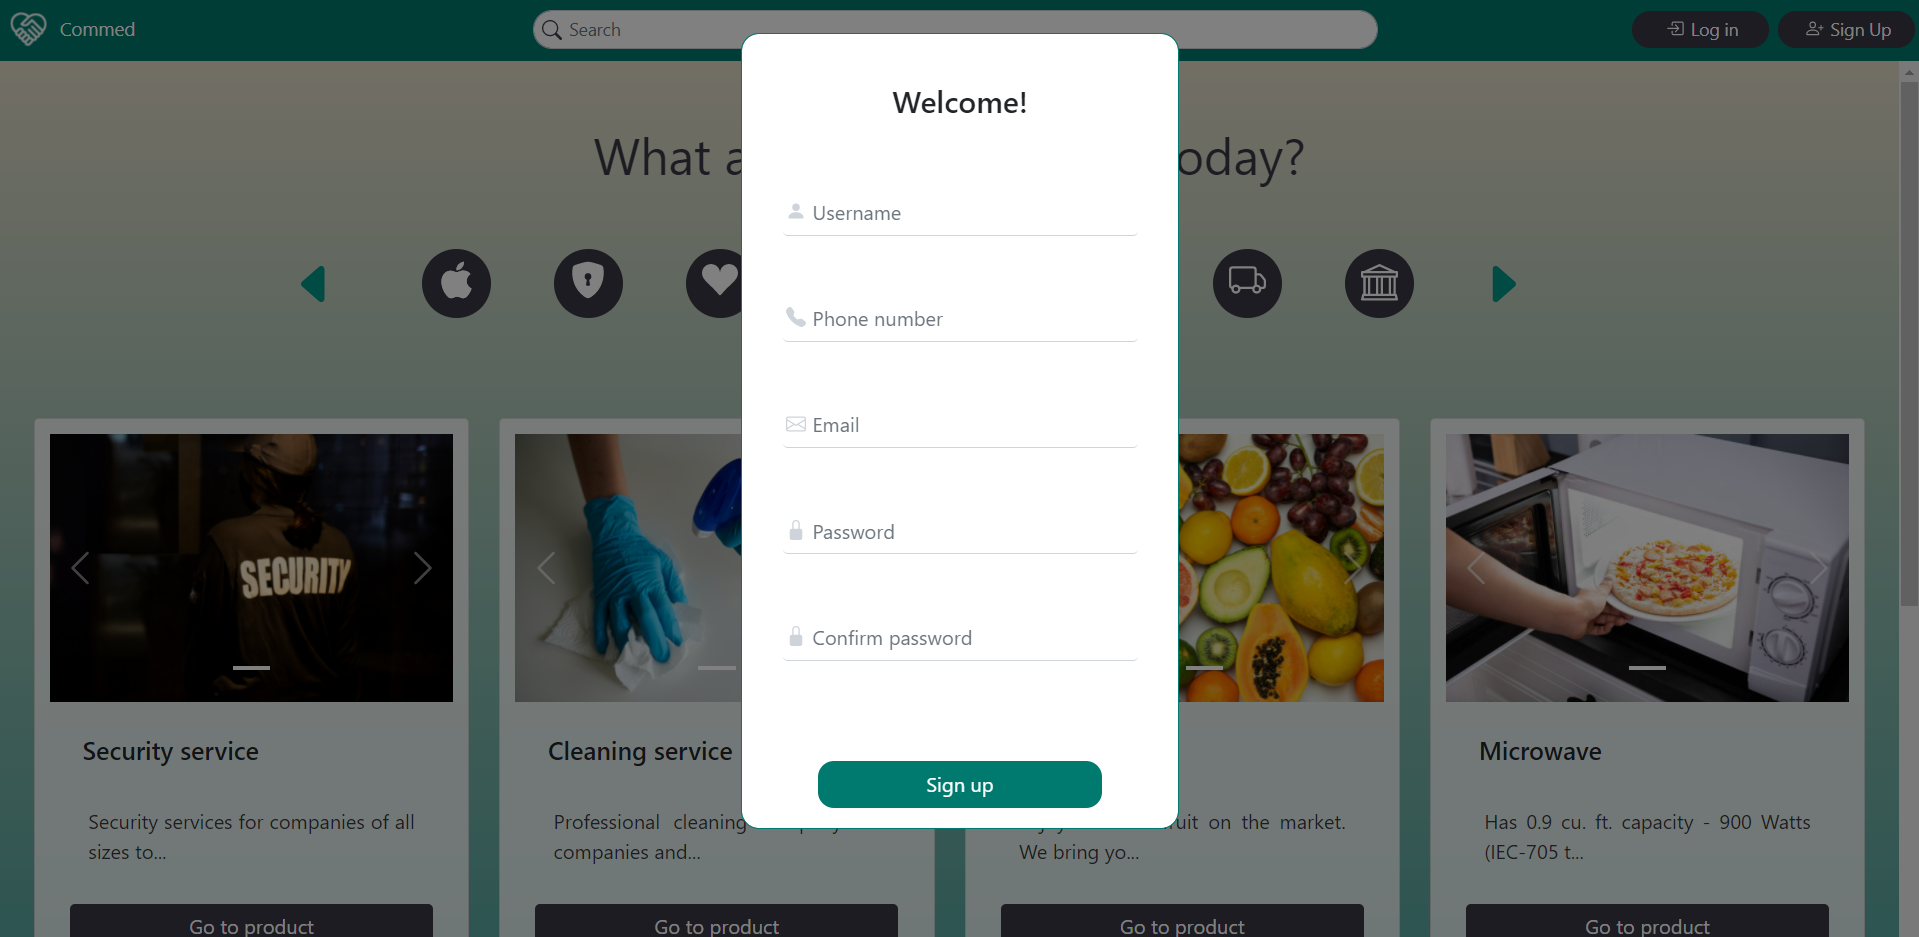
\includegraphics[width=0.5\linewidth]{img/webclient_4.png}
  \caption{Registration screen.}
  \label{fig:webclient-screen-3}
\end{figure}
\begin{figure}[H]
  \centering
  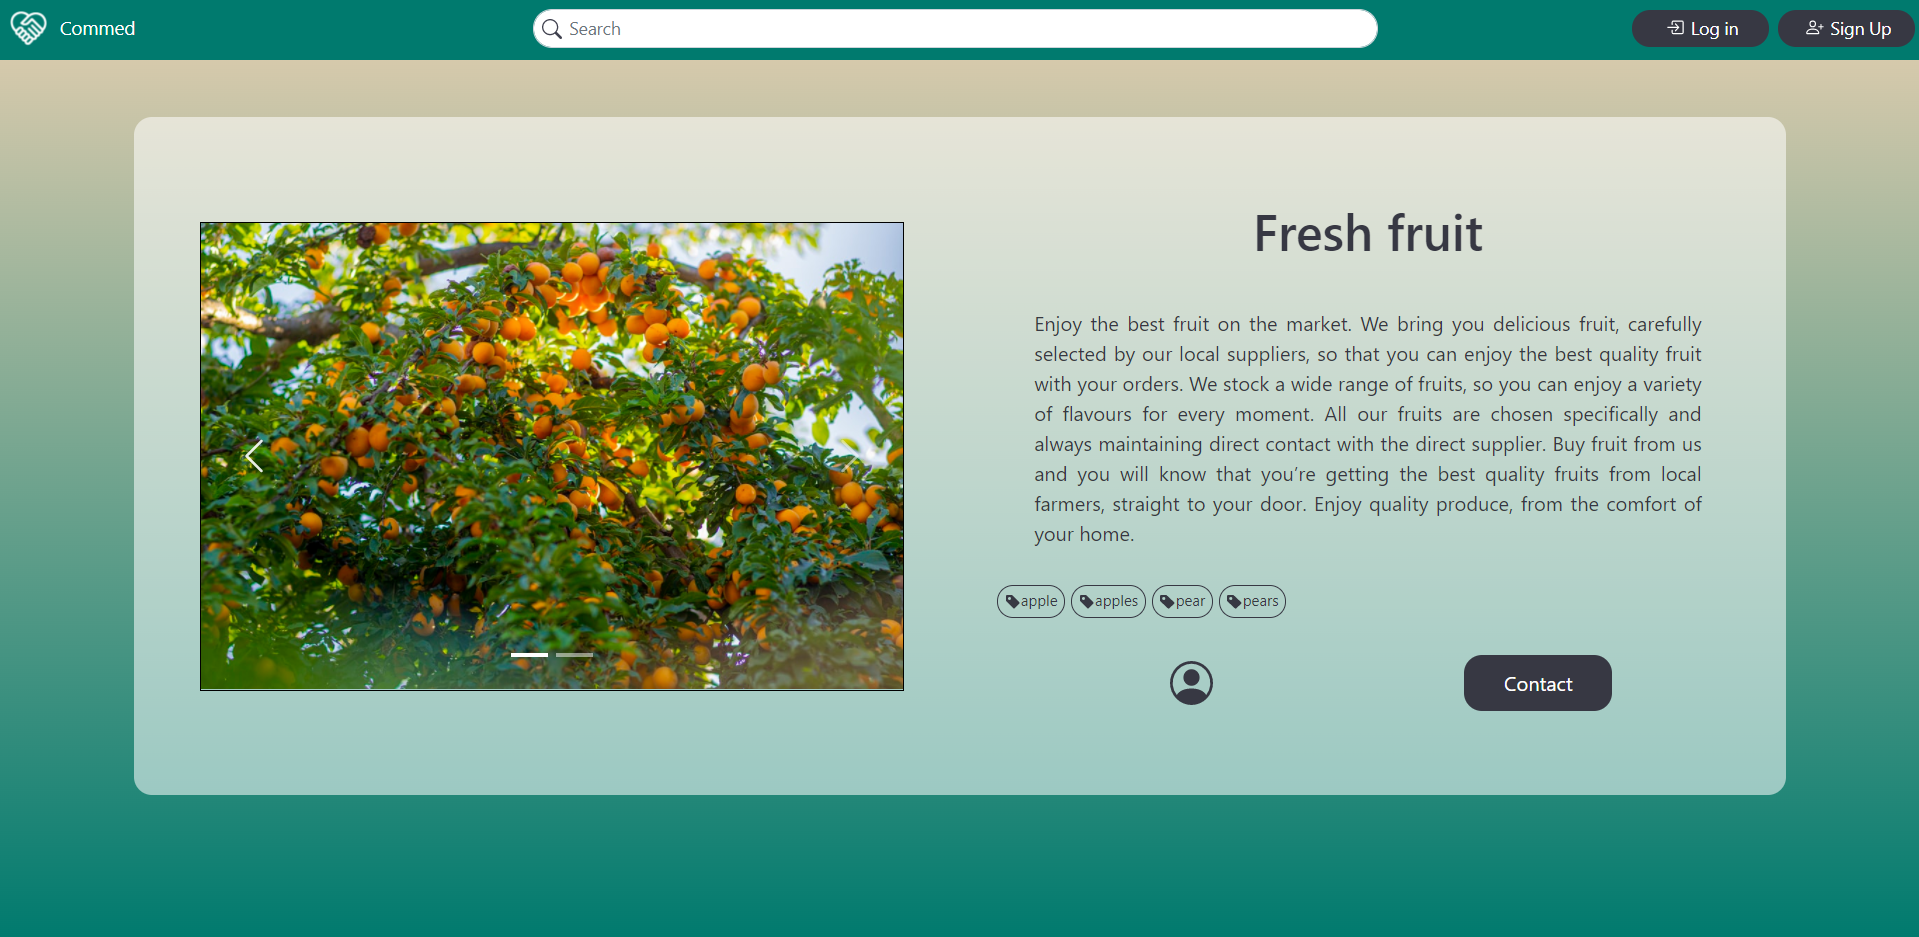
\includegraphics[width=0.5\linewidth]{img/webclient_5.png}
  \caption{Product Details screen.}
  \label{fig:webclient-screen-4}
\end{figure}
\begin{figure}[H]
  \centering
  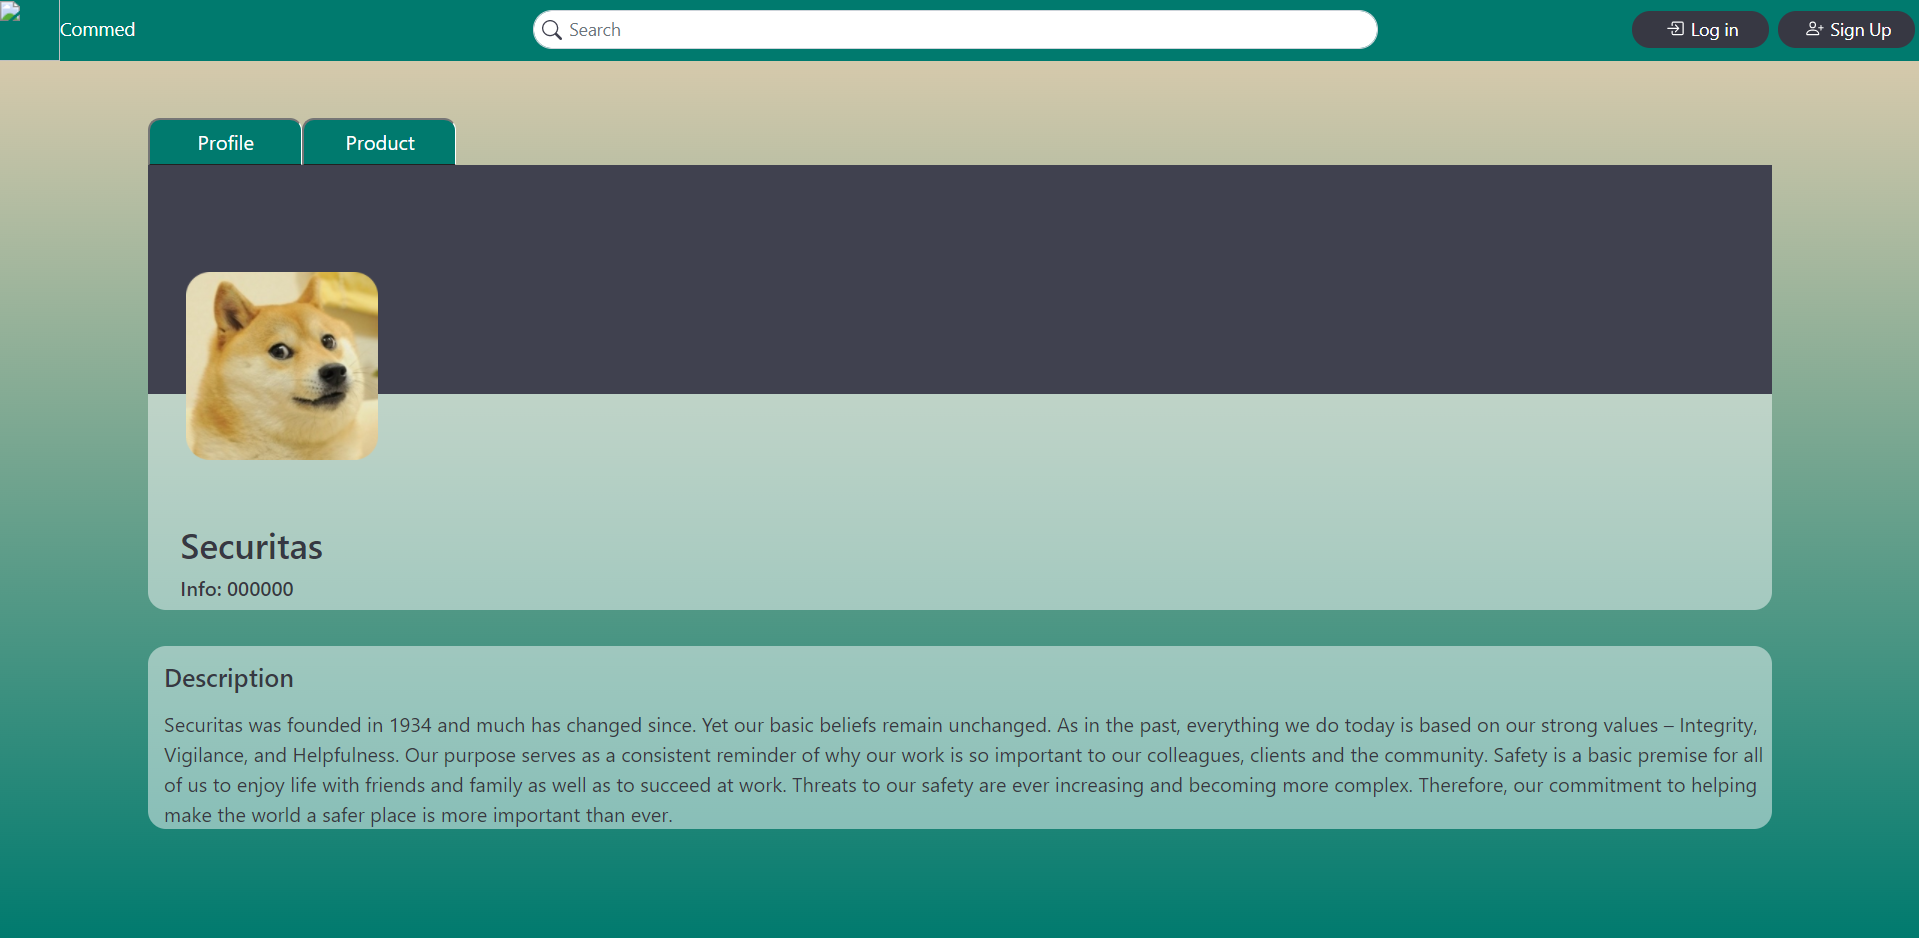
\includegraphics[width=0.5\linewidth]{img/webclient_6.png}
  \caption{Profile screen.}
  \label{fig:webclient-screen-5}
\end{figure}
\begin{figure}[H]
  \centering
  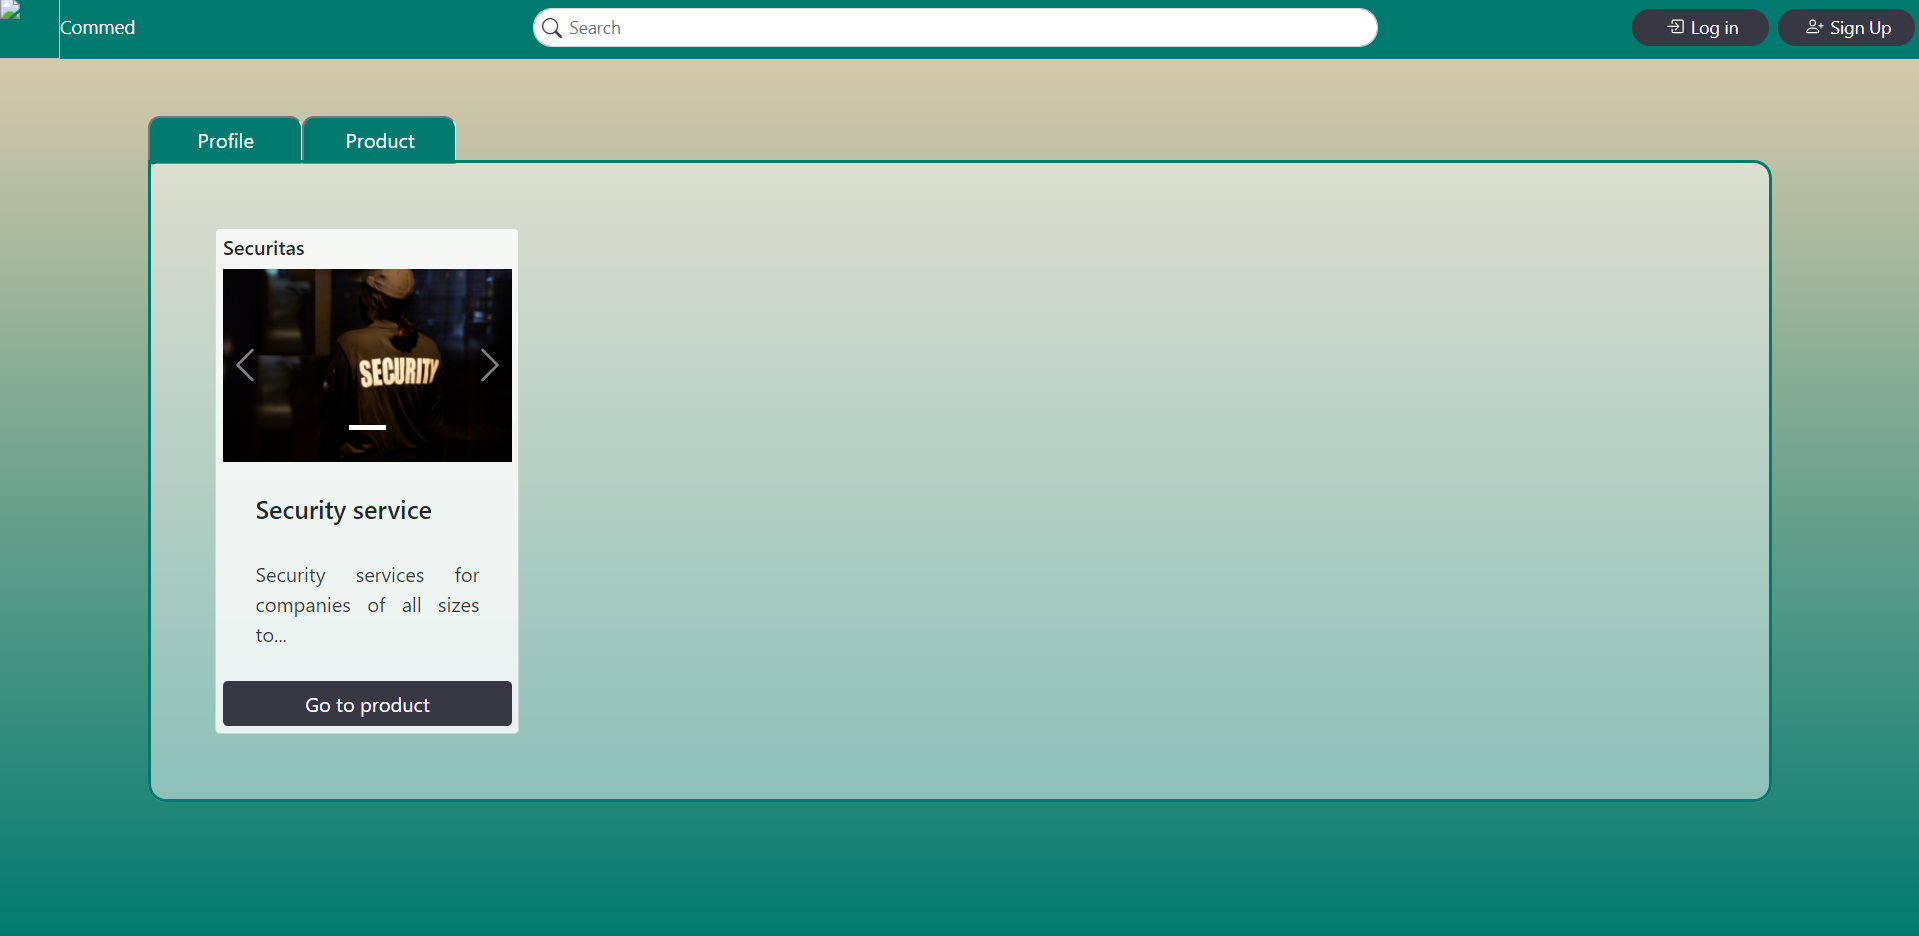
\includegraphics[width=0.5\linewidth]{img/webclient_7.png}
  \caption{Profile Products screen.}
  \label{fig:webclient-screen-6}
\end{figure}
\begin{figure}[H]
  \centering
  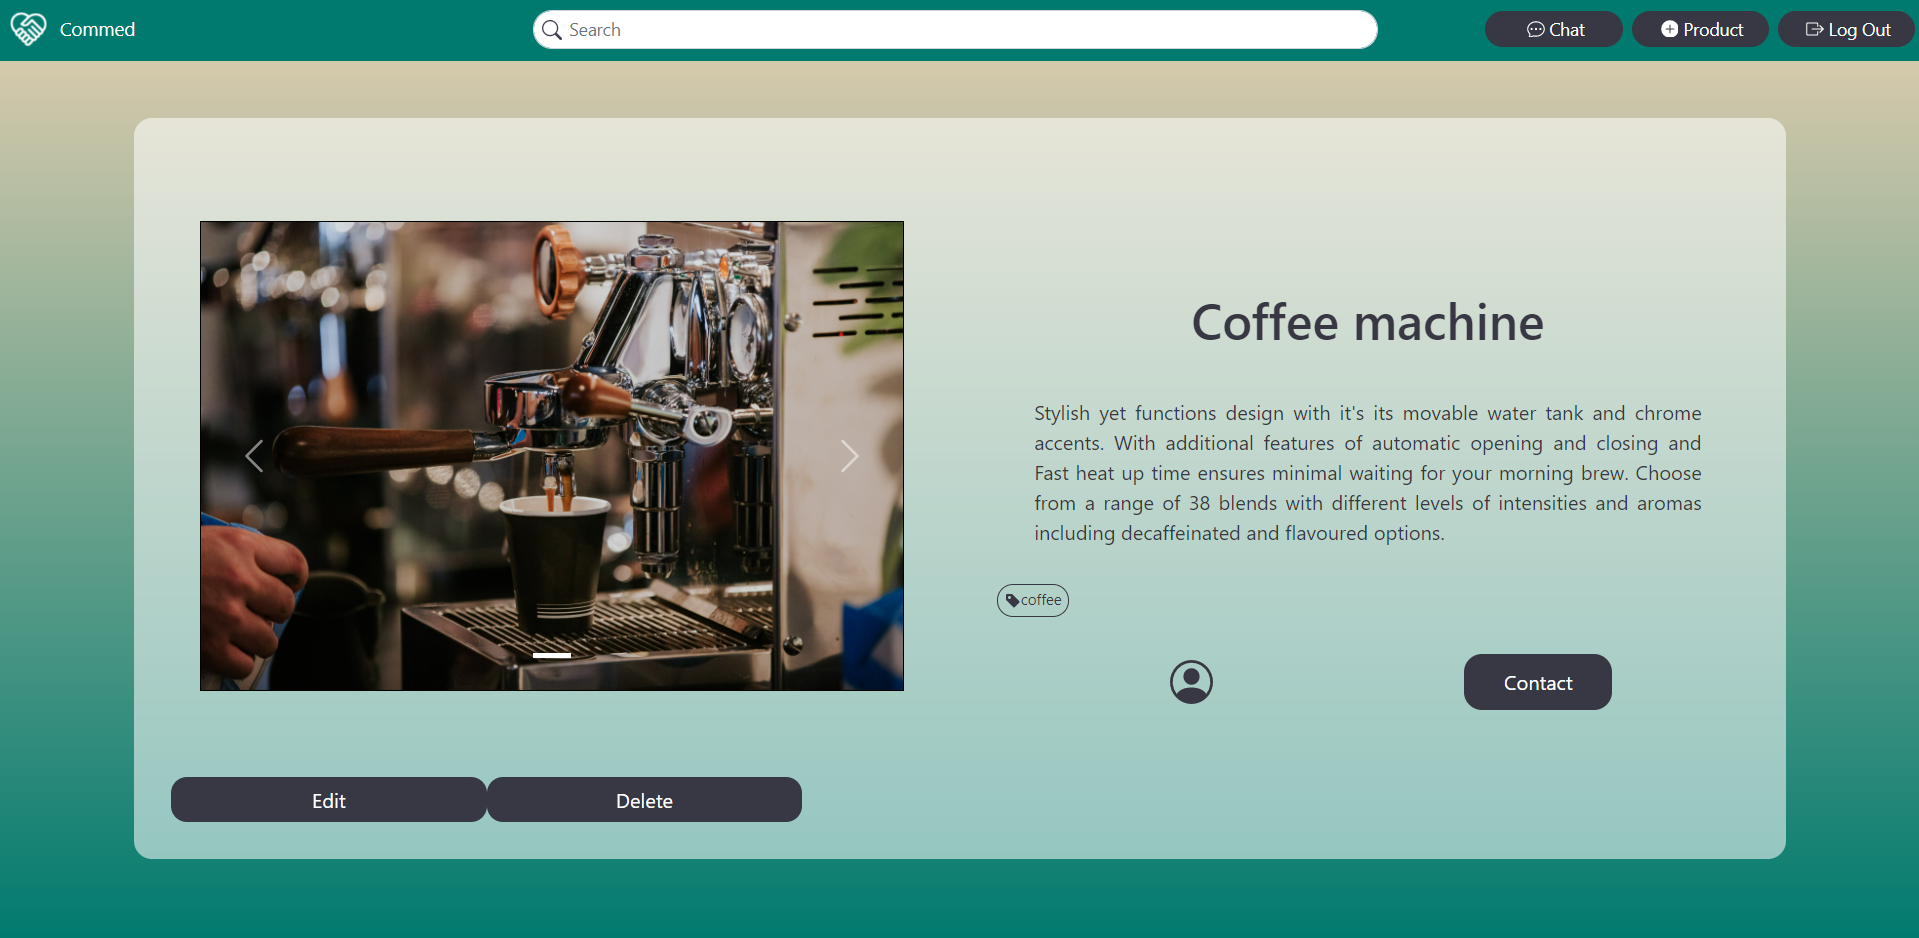
\includegraphics[width=0.5\linewidth]{img/webclient_8.png}
  \caption{Profile Products Loged In screen.}
  \label{fig:webclient-screen-7}
\end{figure}
\begin{figure}[H]
  \centering
  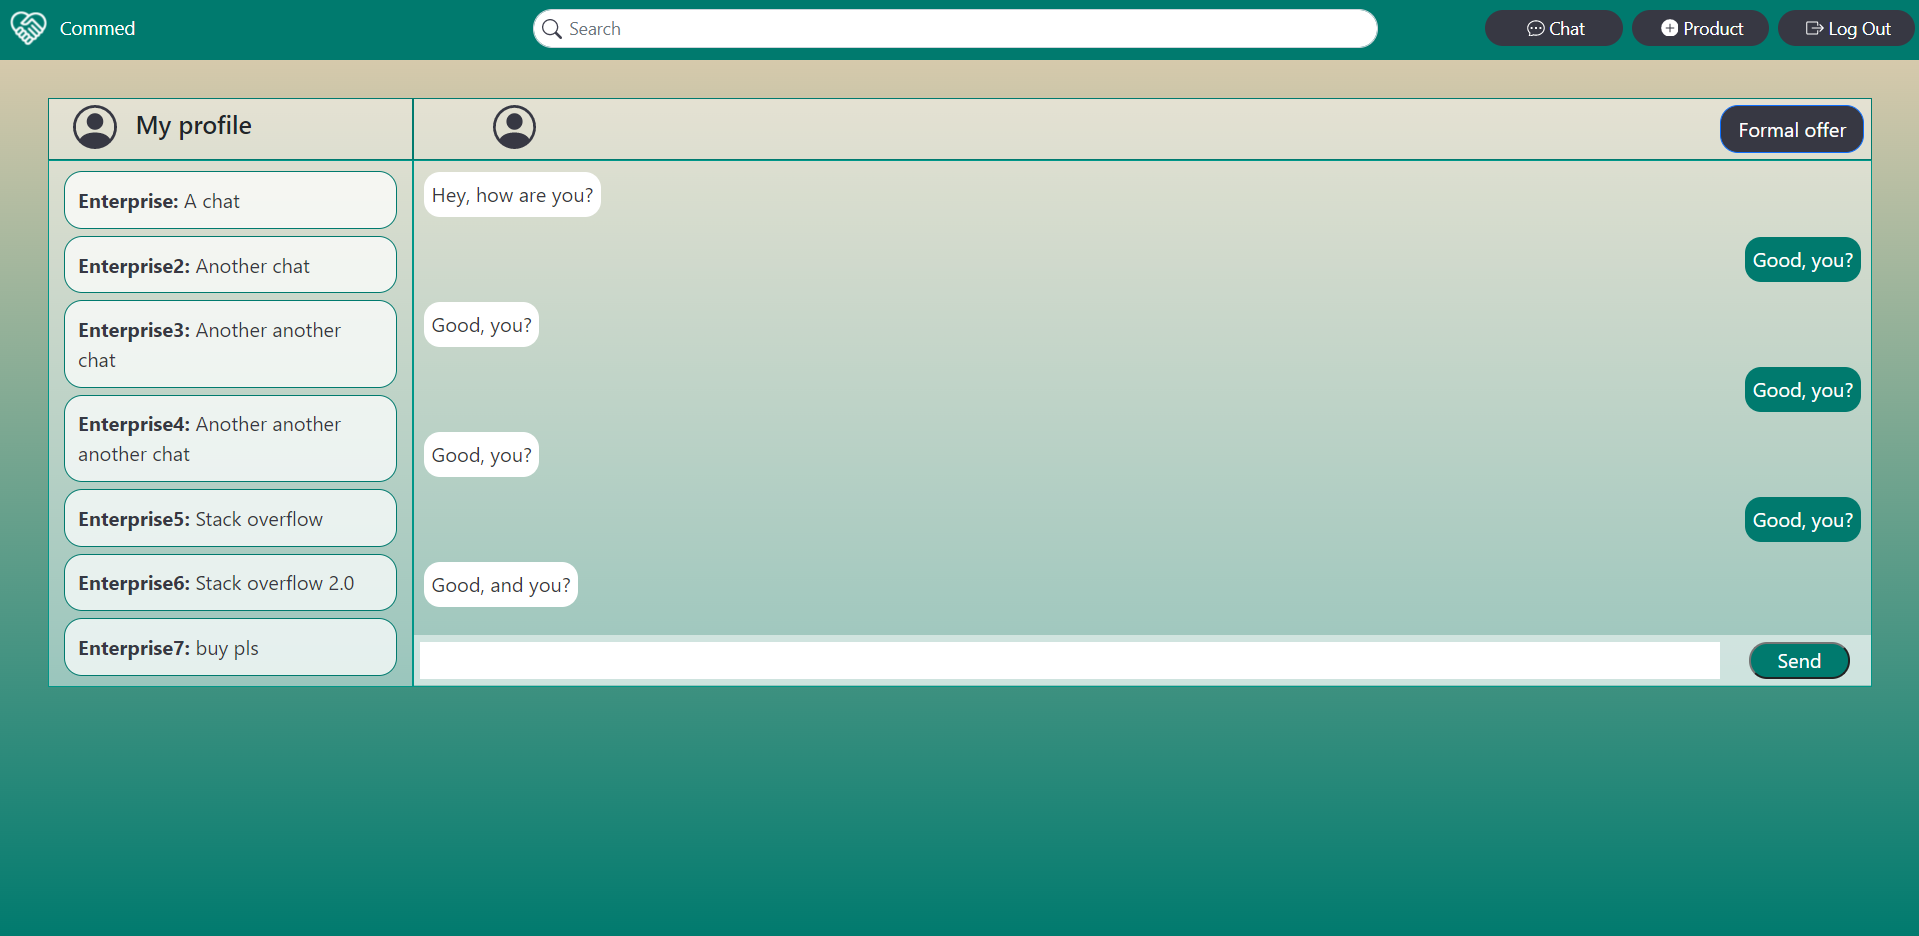
\includegraphics[width=0.5\linewidth]{img/webclient_9.png}
  \caption{Chat screen.}
  \label{fig:webclient-screen-8}
\end{figure}
\begin{figure}[H]
  \centering
  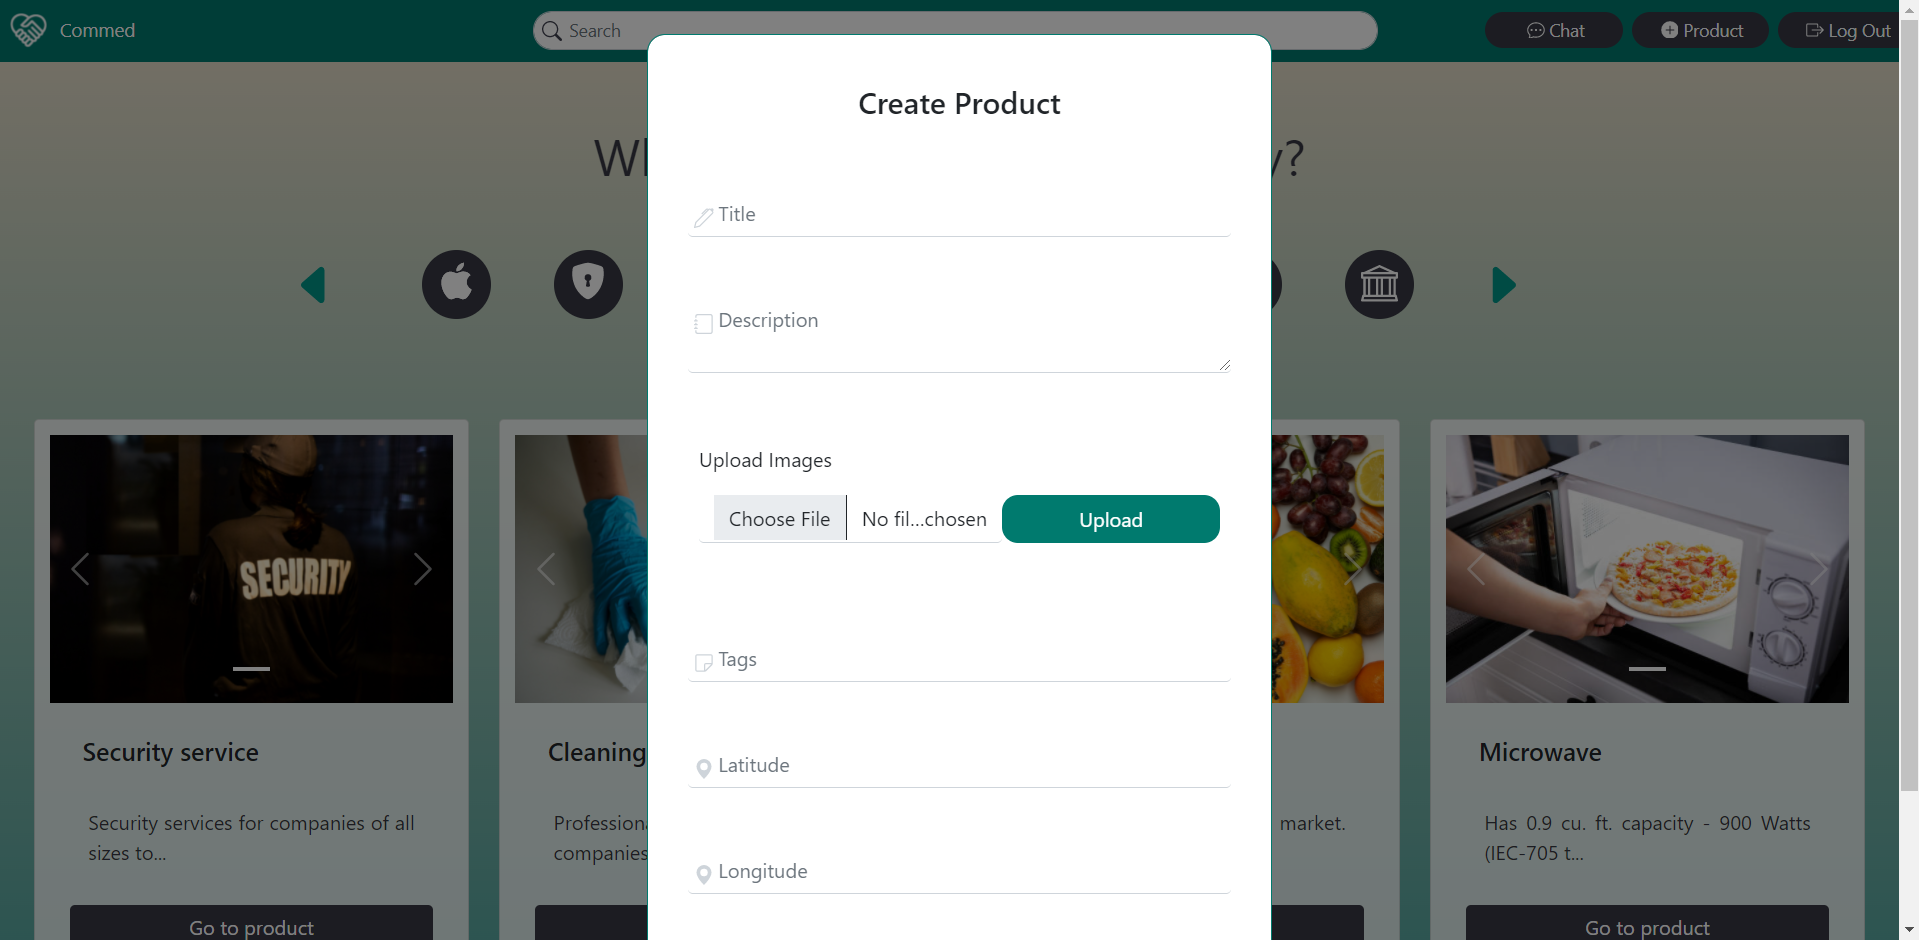
\includegraphics[width=0.5\linewidth]{img/webclient_10.png}
  \caption{Create Product screen.}
  \label{fig:webclient-screen-9}
\end{figure}
\begin{figure}[H]
  \centering
  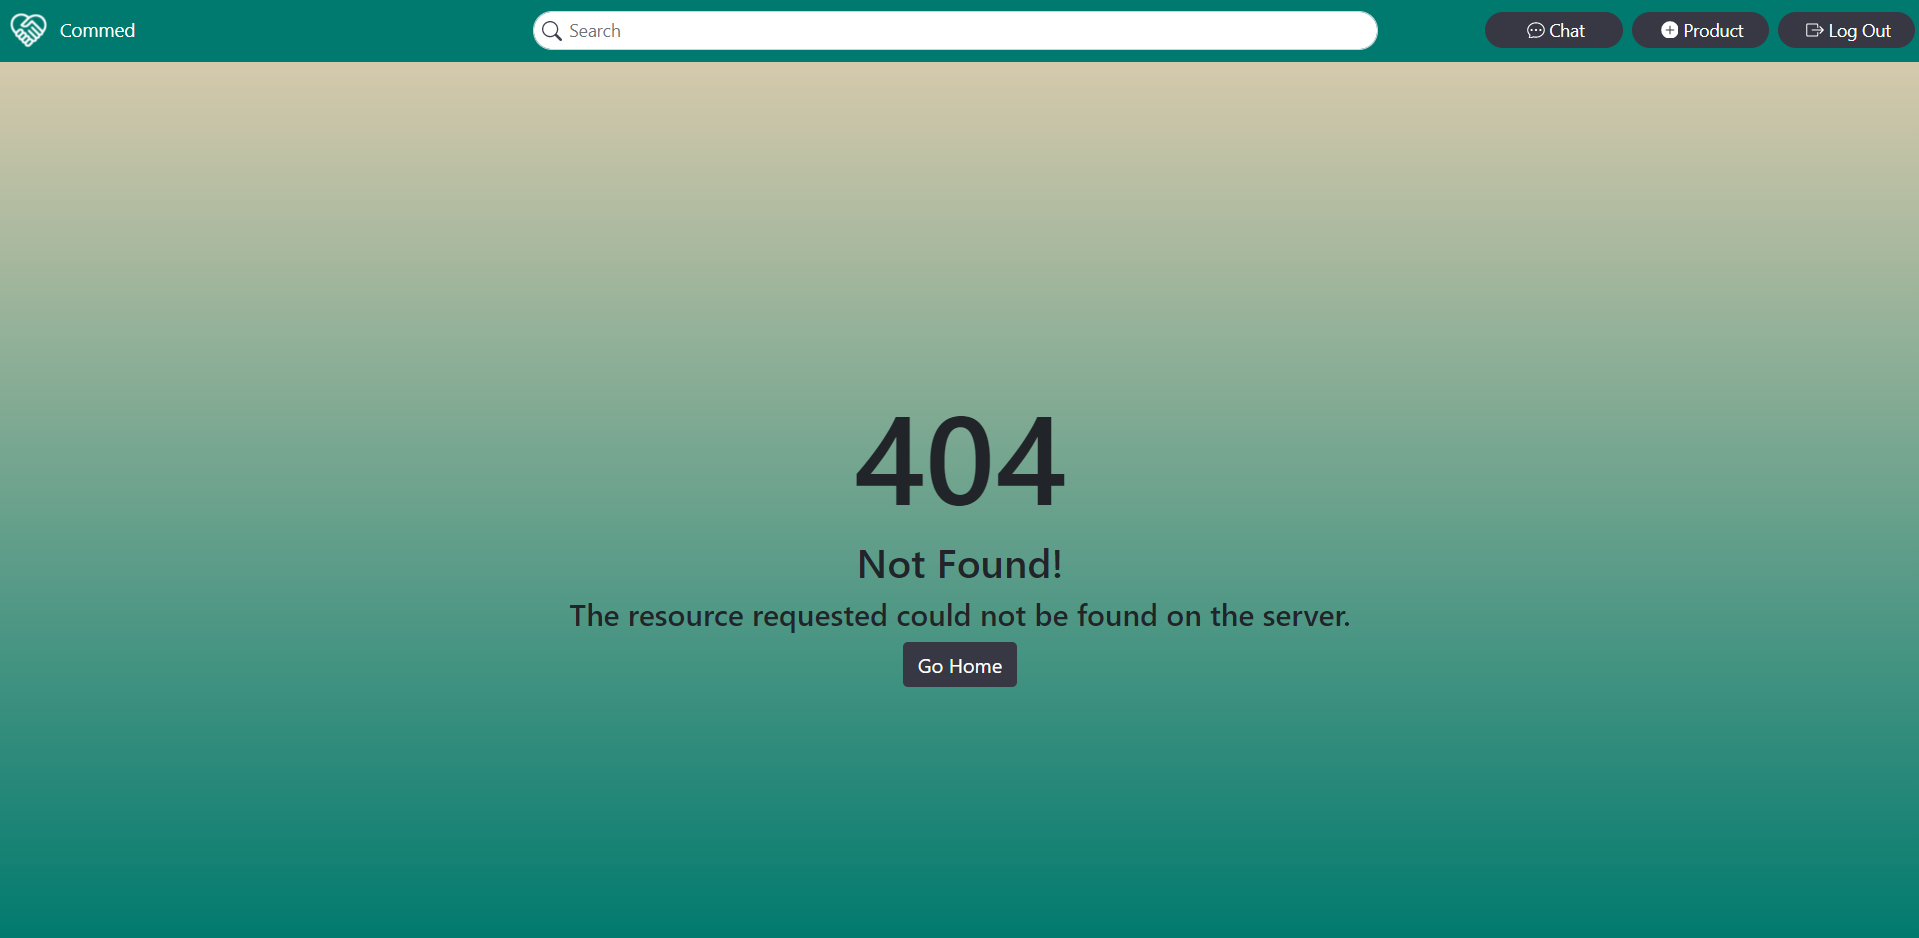
\includegraphics[width=0.5\linewidth]{img/webclient_11.png}
  \caption{404 screen.}
  \label{fig:webclient-screen-10}
\end{figure}
\begin{figure}[H]
  \centering
  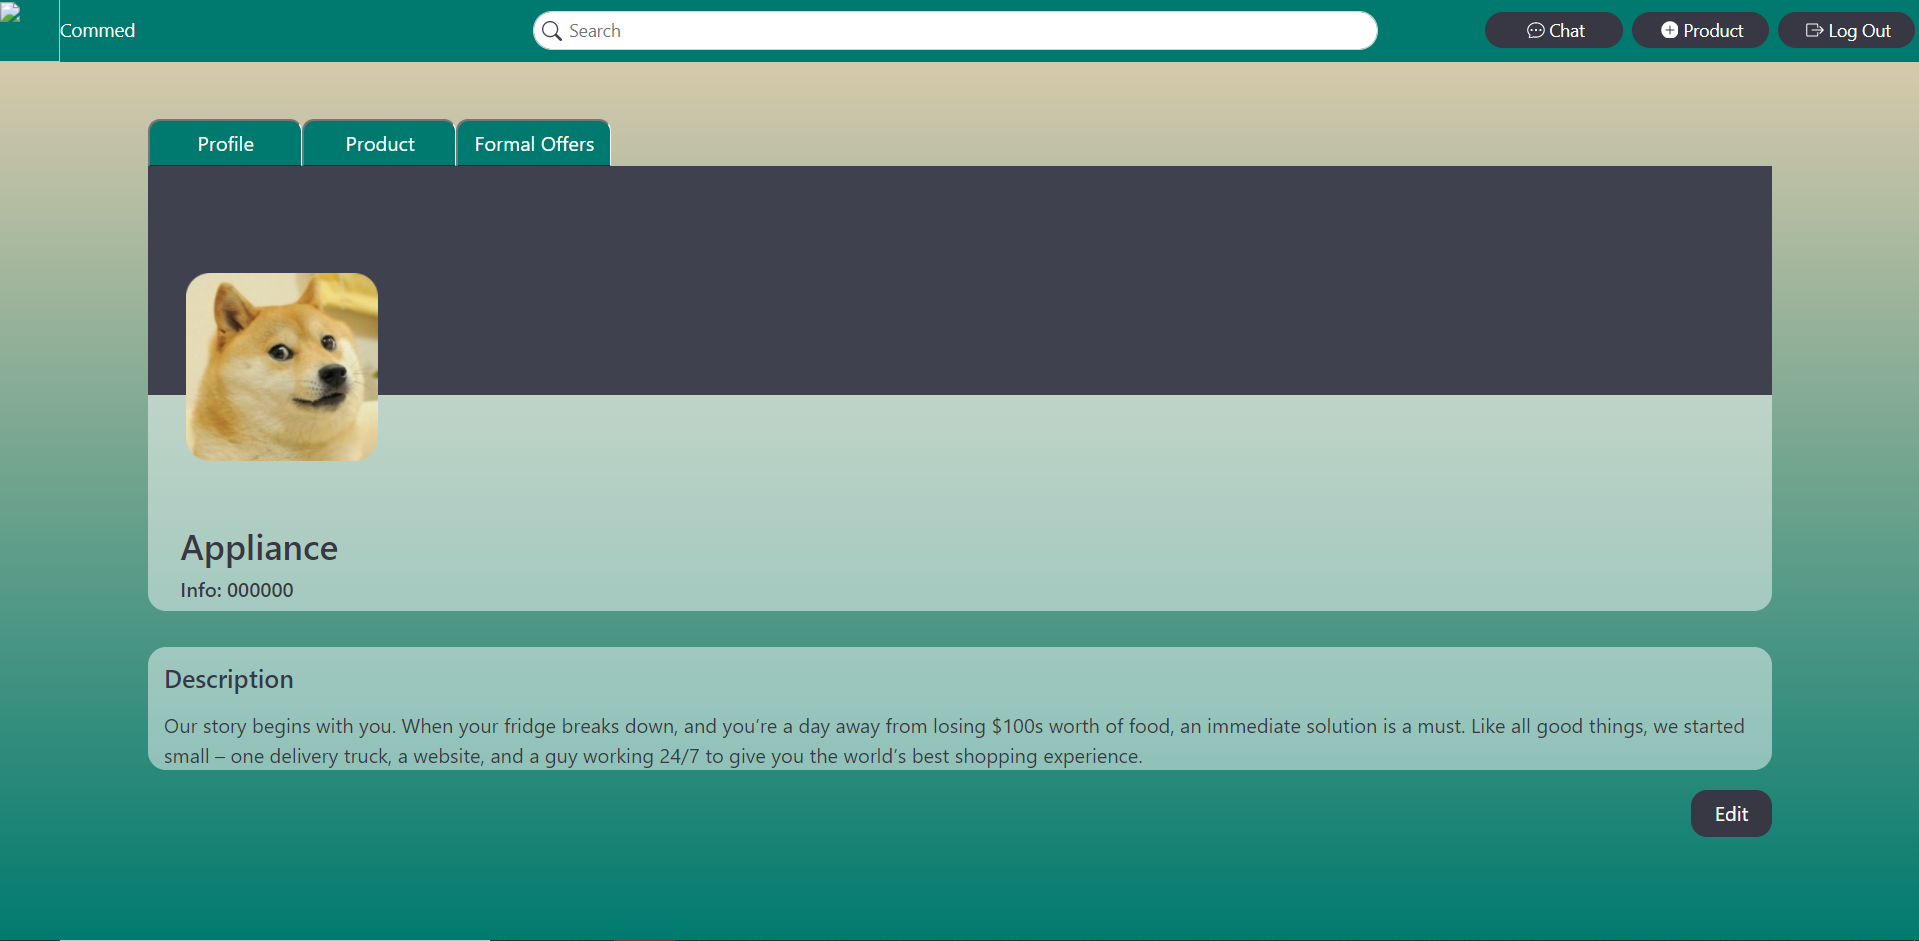
\includegraphics[width=0.5\linewidth]{img/webclient_13.png}
  \caption{Edit screen.}
  \label{fig:webclient-screen-11}
\end{figure}
\begin{figure}[H]
  \centering
  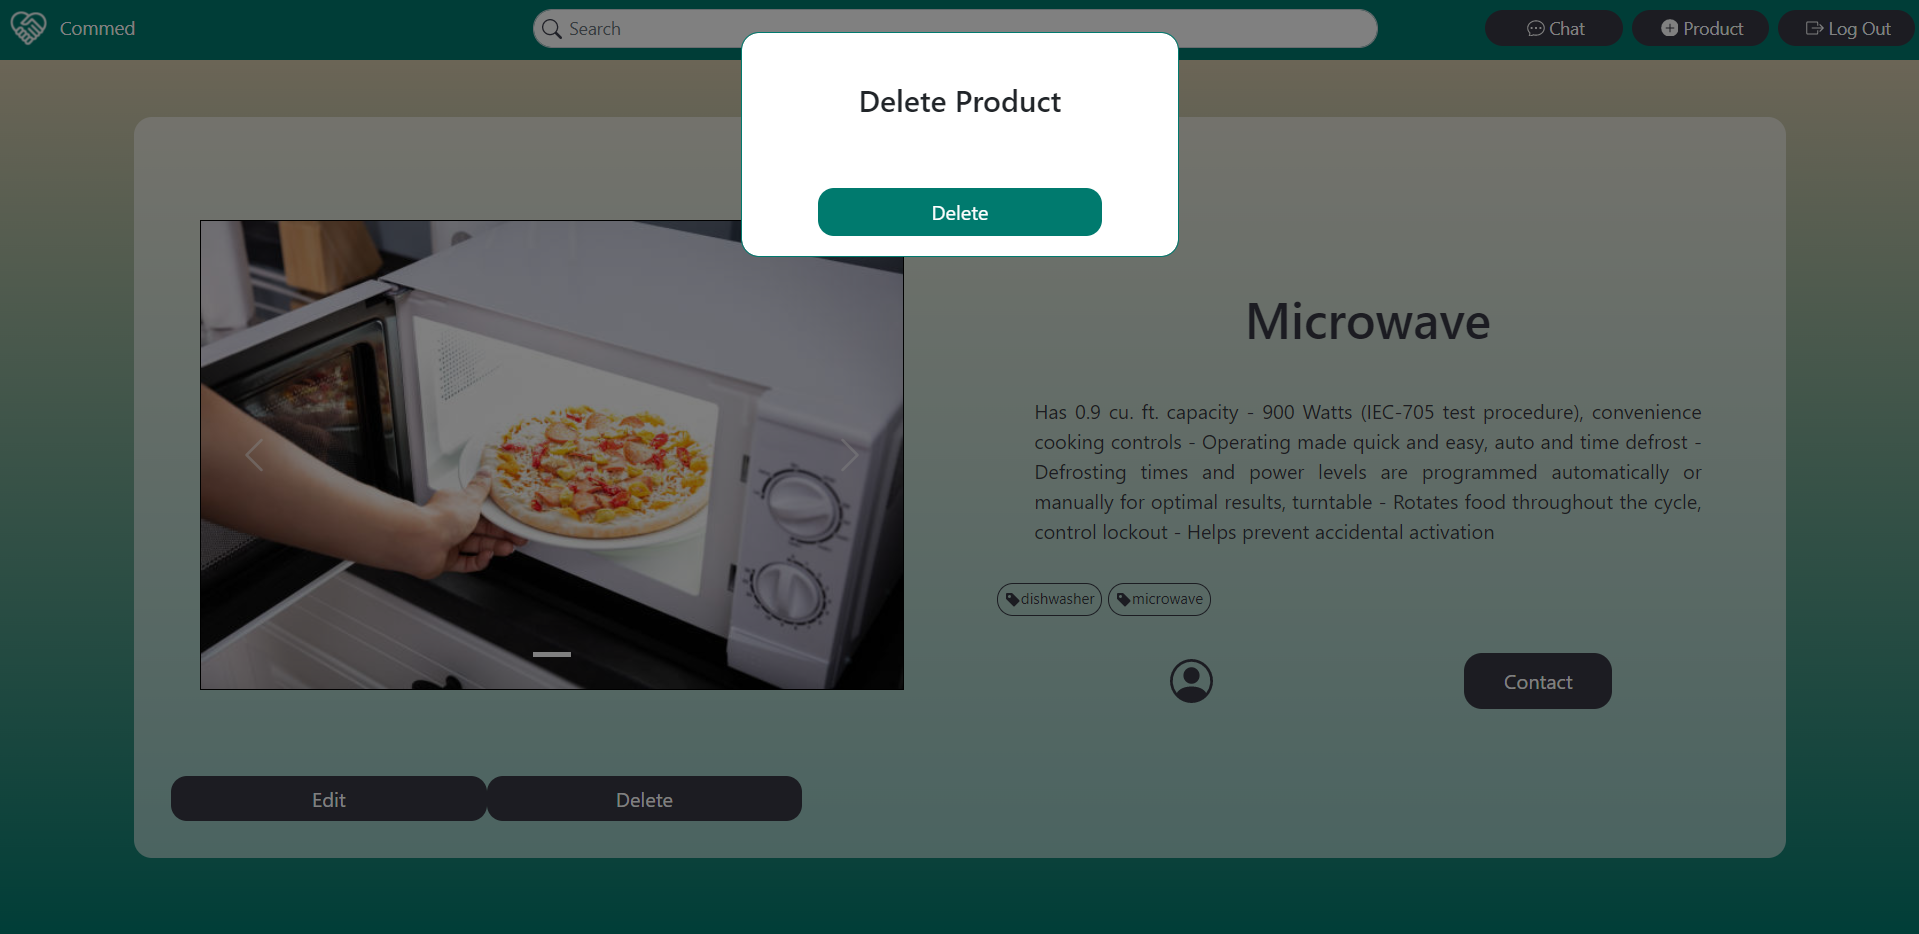
\includegraphics[width=0.5\linewidth]{img/webclient_14.png}
  \caption{Profile Loged In screen.}
  \label{fig:webclient-screen-12}
\end{figure}
\begin{figure}[H]
  \centering
  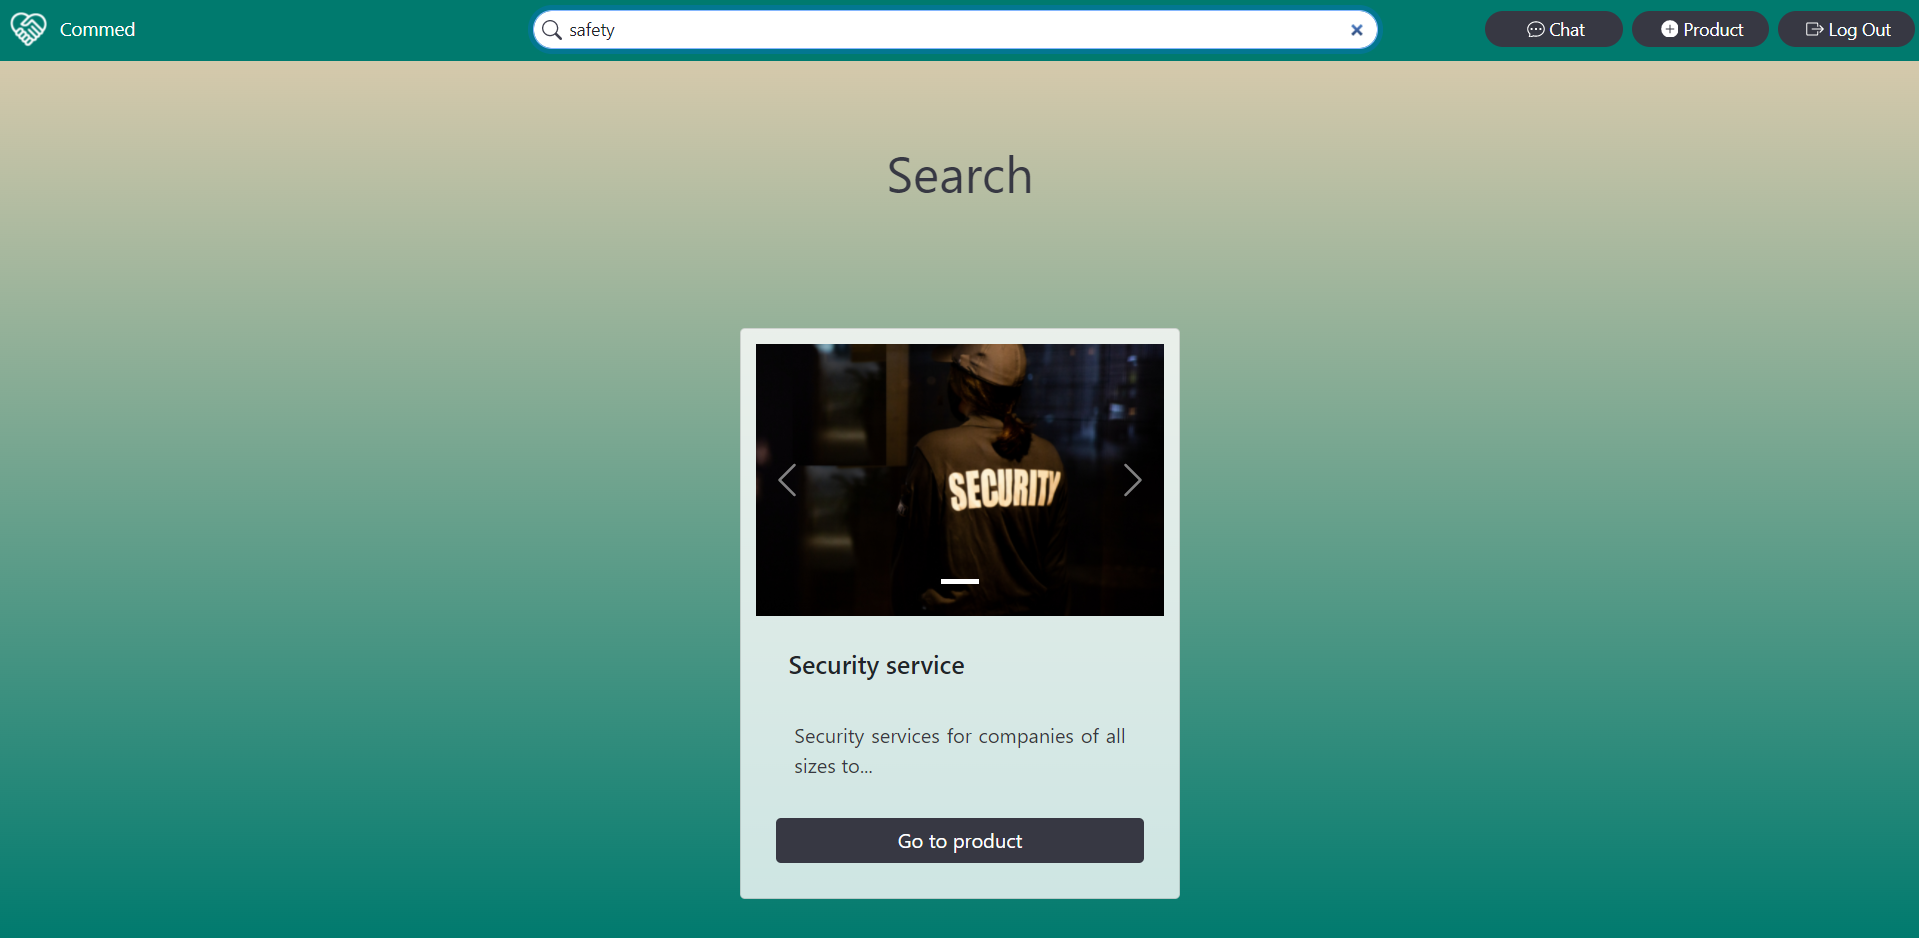
\includegraphics[width=0.5\linewidth]{img/webclient_15.png}
  \caption{Delete Product screen.}
  \label{fig:webclient-screen-13}
\end{figure}
\begin{figure}[H]
  \centering
  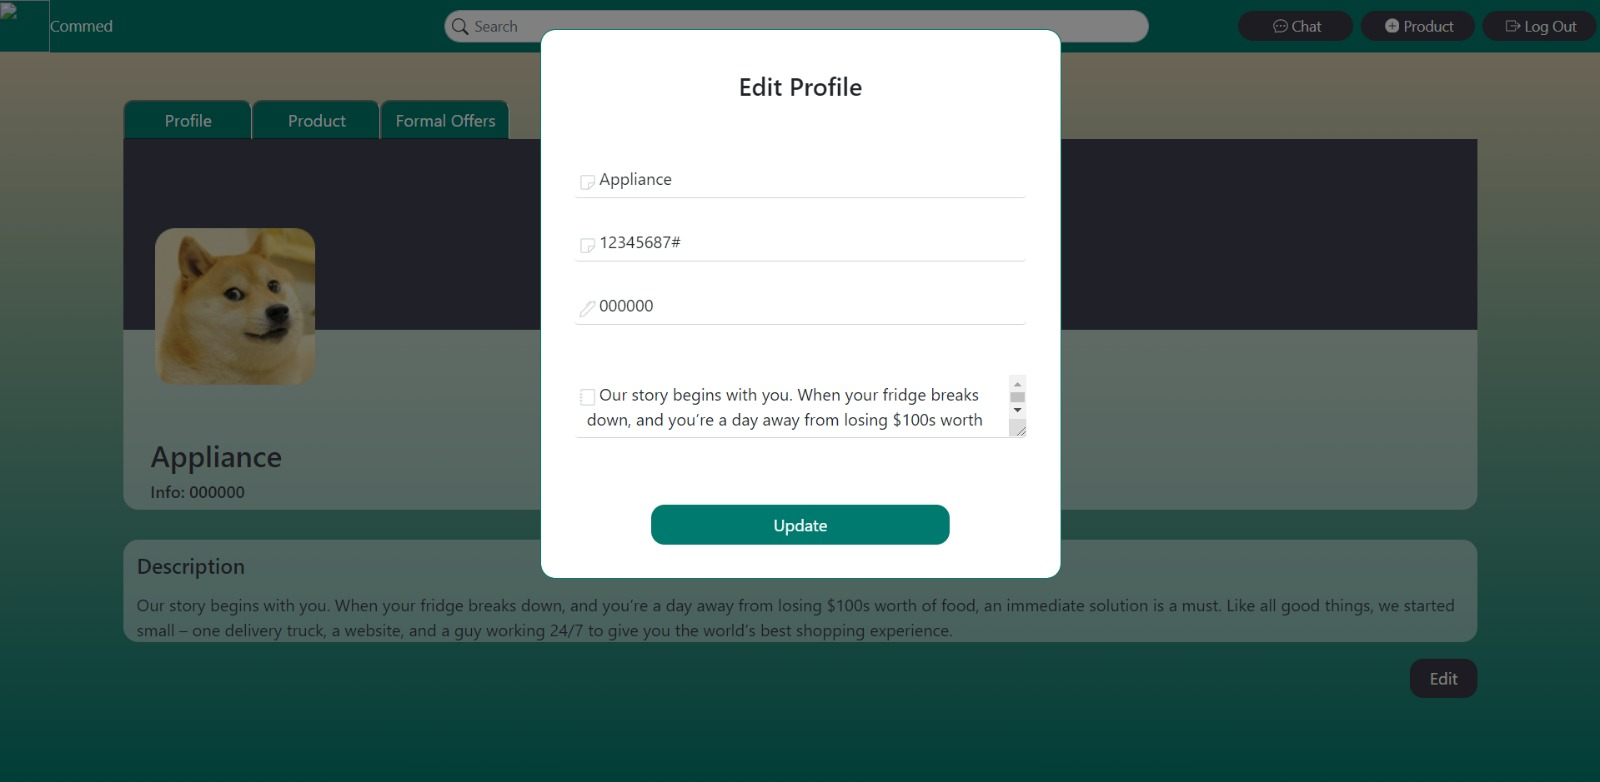
\includegraphics[width=0.5\linewidth]{img/webclient-16.jpg}
  \caption{Search screen.}
  \label{fig:webclient-screen-14}
\end{figure}


\section{Dailies}

\subsection{01-11-2021}
\begin{itemize}
\item Creation of the state diagram of the Mobile Application.
\item Accorded that Jass was going to be the responsible of doing the Wireframe of the application.
\item Accorded that Quim and Emina are working on the React Web Client
\item Accorded that Sergi and Oriol are working with the Flutter Mobile App
\end{itemize}

\subsection{02-11-2021}
\begin{itemize}
\item Talked a little bit about the style of the application
\item Emina and Quim started With Wireframe
\item Mobile Aplication Team started also with the design and the Wireframe of the application.
\end{itemize}

\subsection{03-11-2021}
\begin{itemize}
\item Decided the palette of colors we are using oin our app and mobile app
\item Decided the logos that we are using in our web client and App
\item Put In commont design decissions from both subteams.
\item Talked about the work to be done in the rest of the week
\end{itemize}


\subsection{08-11-2021}
\begin{itemize}
\item Update of the status of the project after the week of work
\item Quim and emina showed wireframe of the app and irst steps of the Web app.
\item Jass showed to us some screens of the wireframe, and opened some design discussion.
\item Oriol and sergi showed botom navigation menu, list of products and started.
\end{itemize}


\subsection{09-11-2021}
\begin{itemize}
\item Jass keep the work with wireframe and started to learn some flutter.
\item Oriol and keep with the work and start login and register.
\item Quim and emina start with the arquitecture of the web.
\end{itemize}


\subsection{10-11-2021}
\begin{itemize}
\item Oriol and sergi keep working with register and login
\item Jass working with wireframe and flutter
\item Quim and Emina srat doing Home screen and comunicate with backend
\item Set the amout of work to do for nexct week
\end{itemize}

\subsection{22-11-2021}
\begin{itemize}
\item Update of the current state od the project
\item Oriol and Sergi showed some Mobile App Screens
\item Quim and emina Showed some screens of the client + Session managment and login/register communicating with with backend
\end{itemize}

\subsection{23-11-2021}
\begin{itemize}
\item Sergi and Oriol Working with More mocked screens of the mobile App
\item Quim and Emina also working in some more Screens of the web application
\end{itemize}

\subsection{24-11-2021}
\begin{itemize}
  \item Quim and Emina put on the table dessign questions that had been debated by all
  \item Sergi and Ori Showed to all the group the progression of the app screens and also leaded on some design discussion.
\end{itemize}

\end{document}
